%!TEX root = main.tex
\chapter{Result}\label{chapter:Result}
In this chapter the results of our approach for pose estimation are represented and analyzed. The results are obtained by the new feature-based pose optimization which was developed in Ubitrack Framework. For testing, an artifact scene is created that consists of a marker with id 0272 and size 18 cm and some artificial objects to provide more feature points.

The ground truth data is a video sequence that is provided by the ARTRACK2 \footnote{\url{http://www.ar-tracking.com/products/discontinued/arttrack2/}} cameras with focal length 2.6 mm. In each moment The ARTRACK2 cameras track the monocular camera that is recognizable by passive markers \footnote{\url{http://www.ar-tracking.com/technology/markers/}}. Based on the retrieved tracking data from ARTRACK2, a Ubitrack module is designed to compute the pose of camera relative to marker and the pose of marker relative to camera precisely. 
The resulting video is a pack of 1034 RGB images with corresponding poses for each frame in two log files. \autoref{fig:sample_dataset_marker} shows some sample images of our ground truth data set.

In this chapter, the obtained results are analyzed in several aspects. At first, because the size of ground truth data is very big, three sets of 80 sequential images are selected randomly from our ground truth data set. For all data sets, the camera has the vertical and horizontal translation, rotation, zoom in and zoom out.

In the first test, we analyze the result of each sample data set individually. For each sample data set, the translation errors between the feature-based and the ground truth data samples are compared with the error between the marker-based and the same ground truth data. The errors of rotation (in quaternion degree) are also computed for both cases. furthermore, for each data set, an evaluation test is applied that shows the movement (rotation and translation) of camera for each time stamp such as $t$ and $t+1$ for both feature-based and marker-based approaches. We find the translation and rotation between each consecutive pair of images (for both methods) and then we compute the distance (euclidean distance for translation and degree in quaternion for rotation) between these two methods. 

This evaluation test demonstrates the difference between these two methods independent of other parameters that might have effect on our result such as the initial estimated pose. It also shows how similar are both methods in estimating the movement of the camera. For instance, the translation between the first and the second frames which is computed by the feature-based approach is compared to the translation between the same frames but for the marker-based approach. The distance between this two approaches is computed by the euclidean distance and shows how close are the estimates of two approaches. 

As it was mentioned in \autoref{chapter:pose_estimation}, we introduced two threshold parameters which define the size of a bundle and the number of frames that are involved for updating the 3D world map and global bundle adjustment. They are called local threshold and global threshold respectively. for the first data sample, the performance of the proposed feature-based approach is evaluated for different values of local and global thresholds. Finally, for the first data sample, the performance of the proposed feature-based approach is evaluated based on different methods for initial pose estimation as explained in \autoref{subsec:pose_first_bundle}.

\begin{figure}[H]
\centering
\begin{tabular}{cc}
  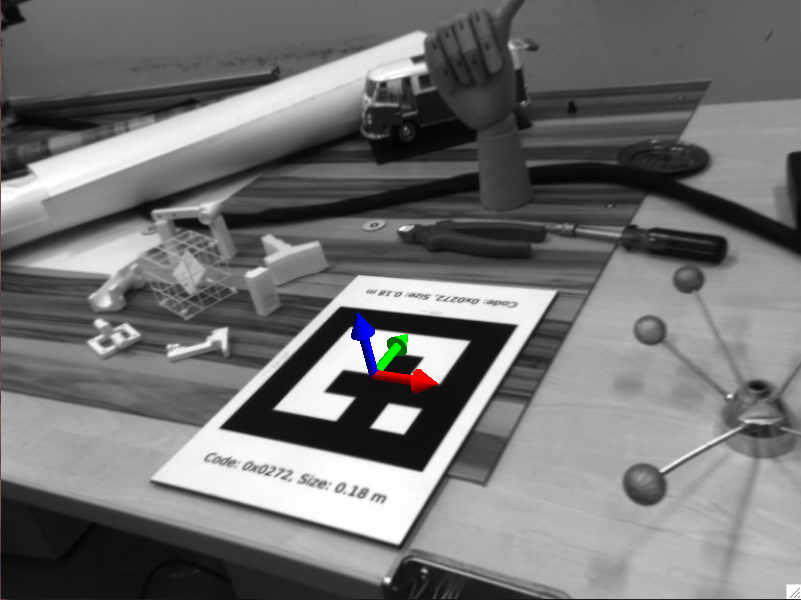
\includegraphics[width=45mm]{figures/sample_0} &   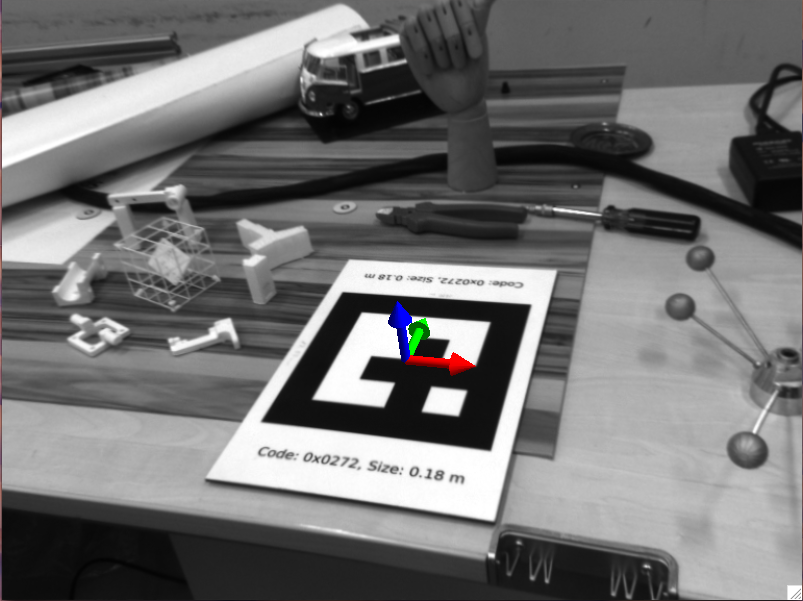
\includegraphics[width=45mm]{figures/sample_1}  \\
  a & b \\[6pt]
  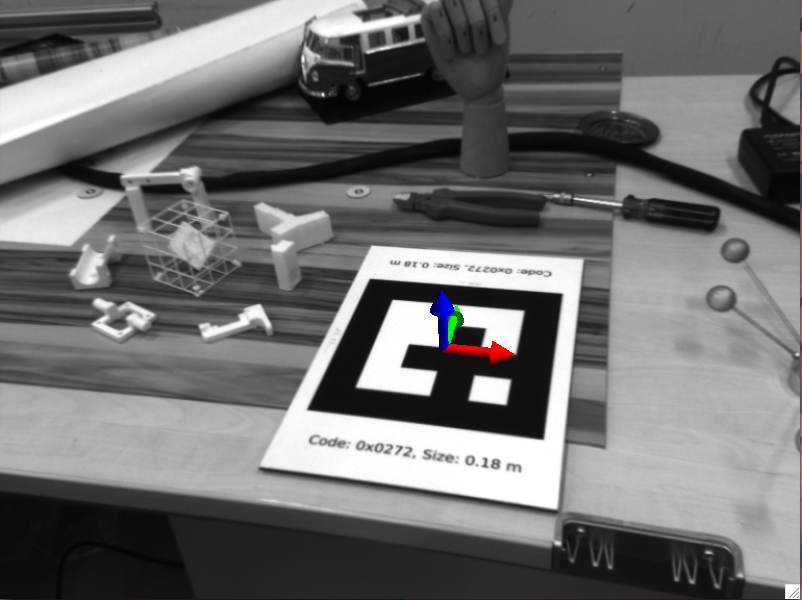
\includegraphics[width=45mm]{figures/sample_2} &   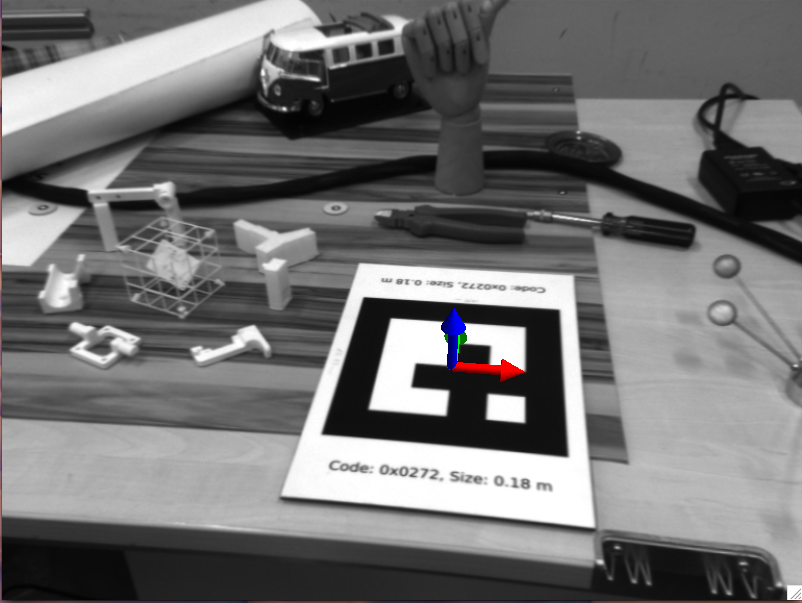
\includegraphics[width=45mm]{figures/sample_3} \\
  c & d \\[6pt]
  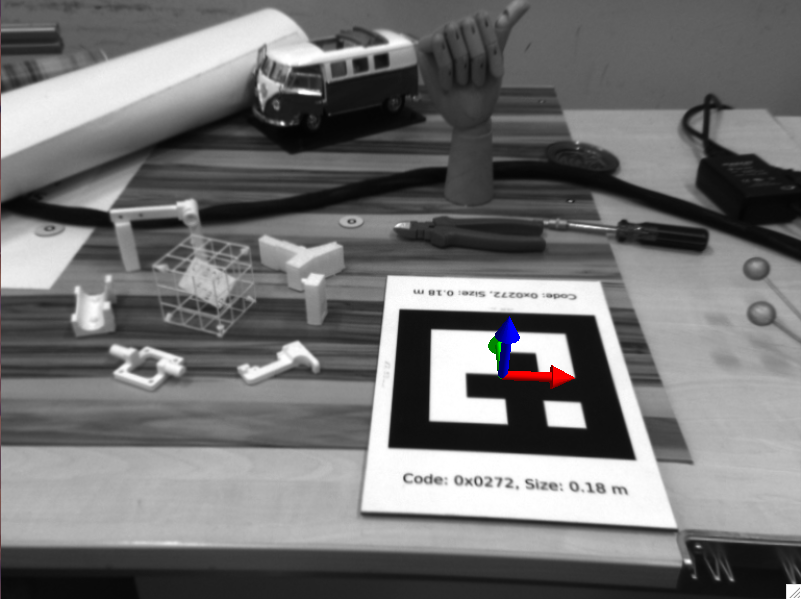
\includegraphics[width=45mm]{figures/sample_4} &   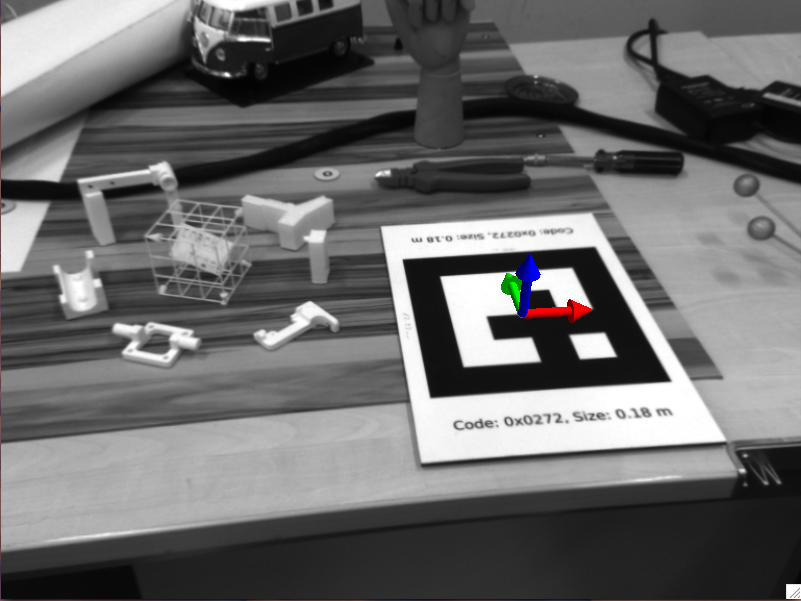
\includegraphics[width=45mm]{figures/sample_5} \\
  e & f \\[6pt]
\end{tabular}
\caption{The sample images of our ground truth data set}\label{fig:sample_dataset_marker}
\end{figure}

\section{Sample Data Set 1} \label{sec:sample_01}
This set consists of 80 sequential images that cover all three types of movement and transformations (horizontal and vertical movement, rotation and zooming). in feature-based case, we assume that the initial pose for the first bundle are provided by the reference system.

\begin{figure}[H]
\begin{tabular}{cc}
  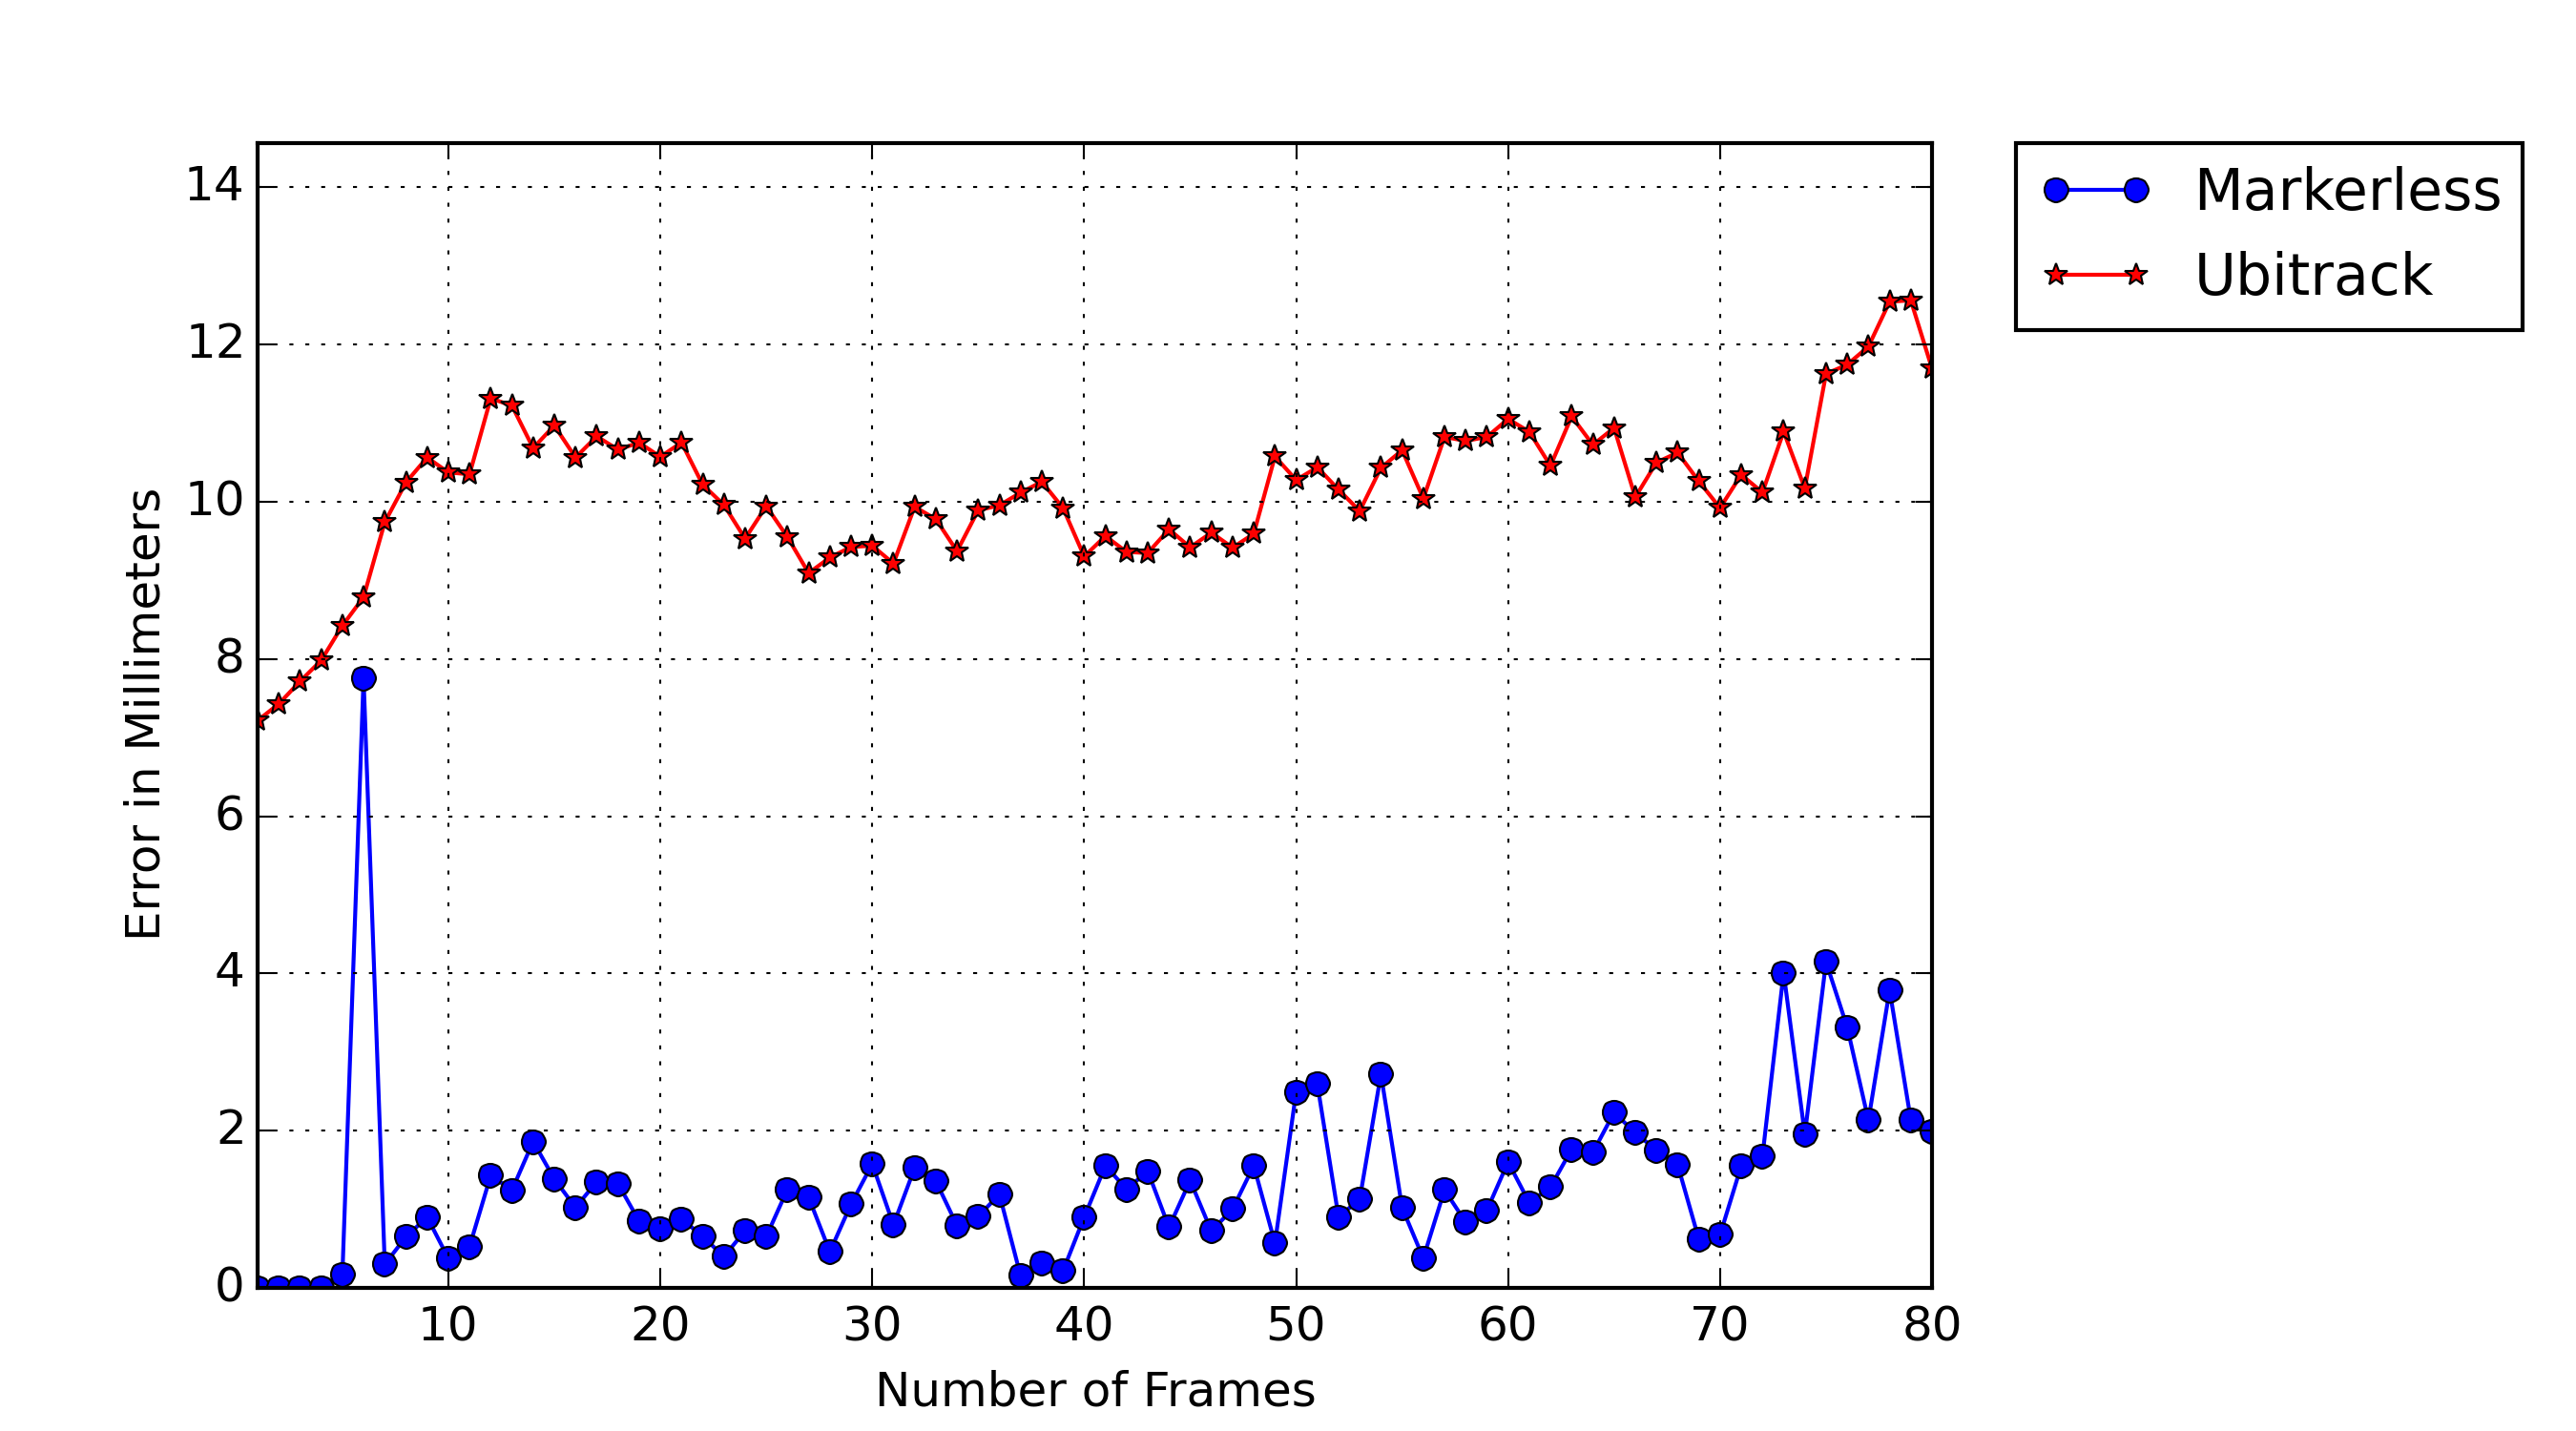
\includegraphics[width=80mm]{figures/global_35/graph_translation} &  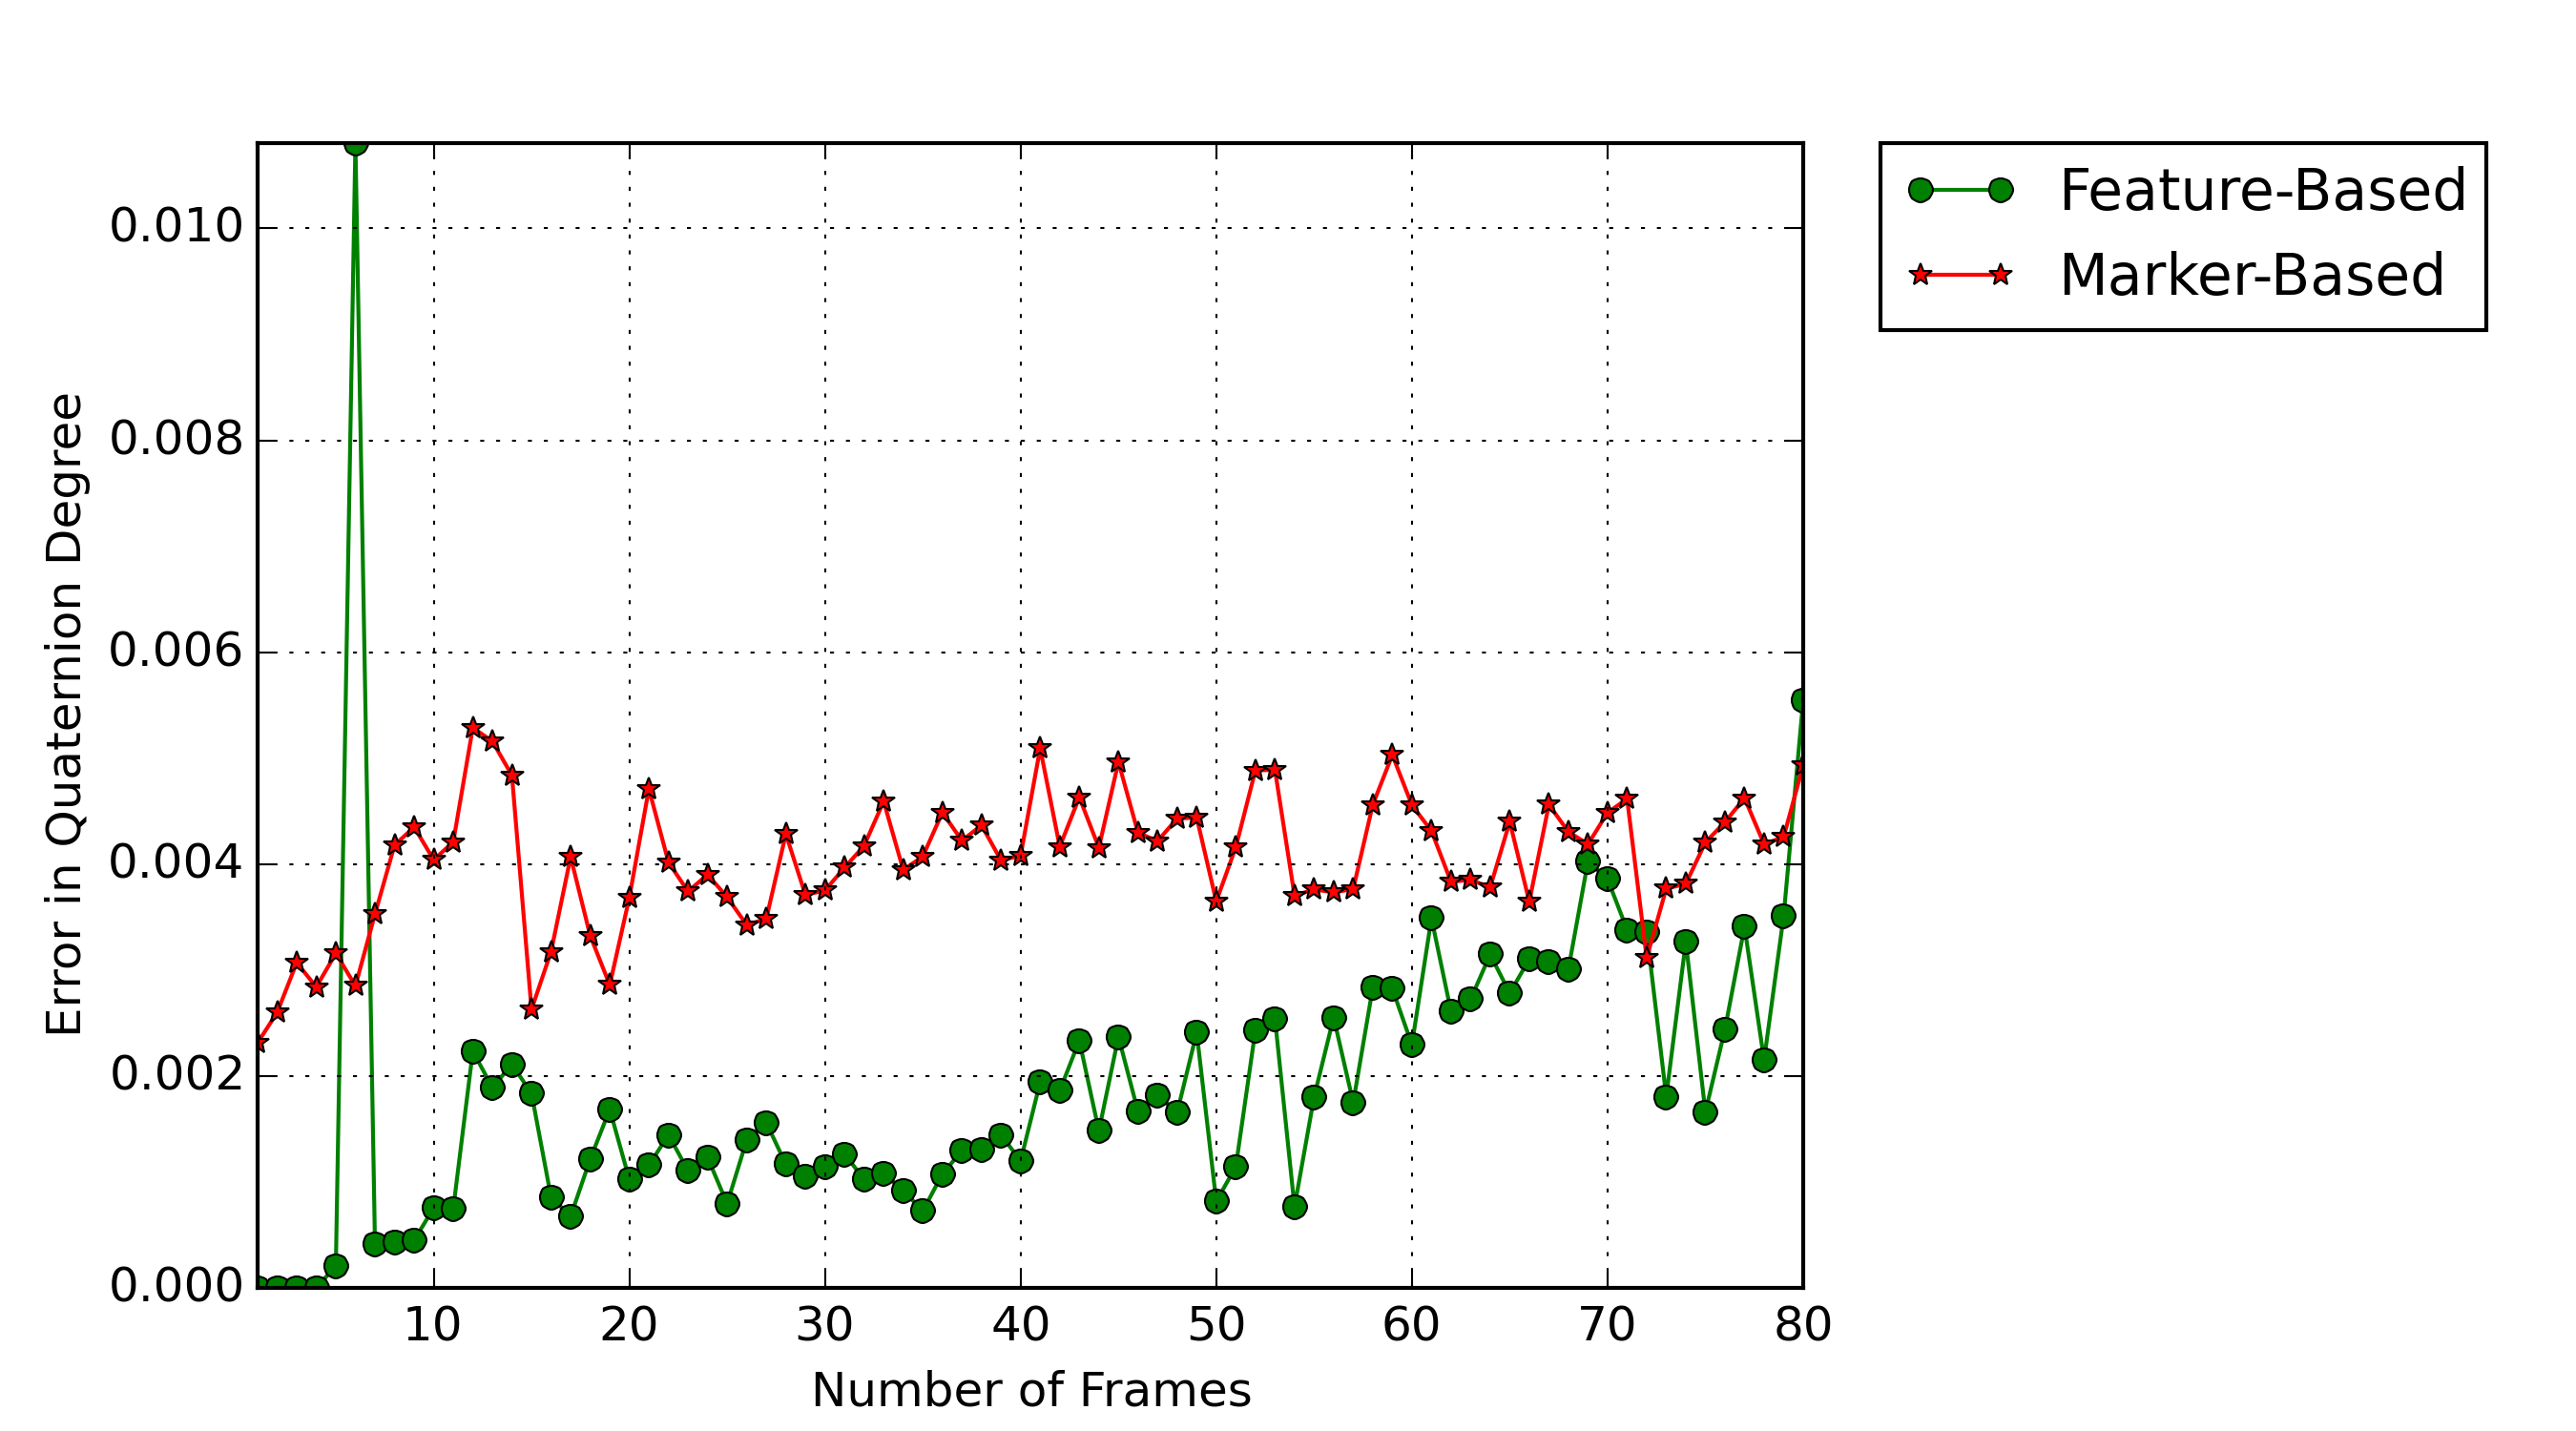
\includegraphics[width=80mm]{figures/global_35/graph_rotation} \\
(a) The translation error & (b) The rotation error \\[6pt]
\end{tabular}
\caption{The tracking errors for both feature-based and marker-based techniques based on the first ground truth data set}   \label{fig:sample_01}
\end{figure}

\begin{table}[H]
\centering
  \begin{tabular}{| c || c | c | c | c |}
      \hline
      & \multicolumn{2}{c|}{Translation} & \multicolumn{2}{c|}{Rotation} \\ \hline
       & Mean & Standard Deviation & Mean & Standard Deviation \\ \hline
      Feature-Based Approach & 1.3303 & 1.1184 & 0.0019 & 0.0015 \\ \hline
      Marker-Base Approach & 10.1552 & 0.9700 & 0.0040 & 0.0006 \\ \hline
  \end{tabular}
  \caption{the statistical analysis of tracking error for both feature-based and marker-based techniques based on the first ground truth data set} \label{tab:sample_01}
\end{table}

Based on both \autoref{fig:sample_01} and \autoref{tab:sample_01}, the tracking result of feature-based is significantly better than marker-based approach for both mean and standard deviation cases. In the case of rotation, the result of marker-less tracking is stable around the 0.0040 degree of quaternion whereas the rotation of feature-based is stable at first but it has a slow increase after the 60th frames. The peak in \autoref{fig:sample_01} (a) and (b) for the 7th image, are the consequence of image blurring. 

\begin{figure}[H]
\begin{tabular}{cc}
  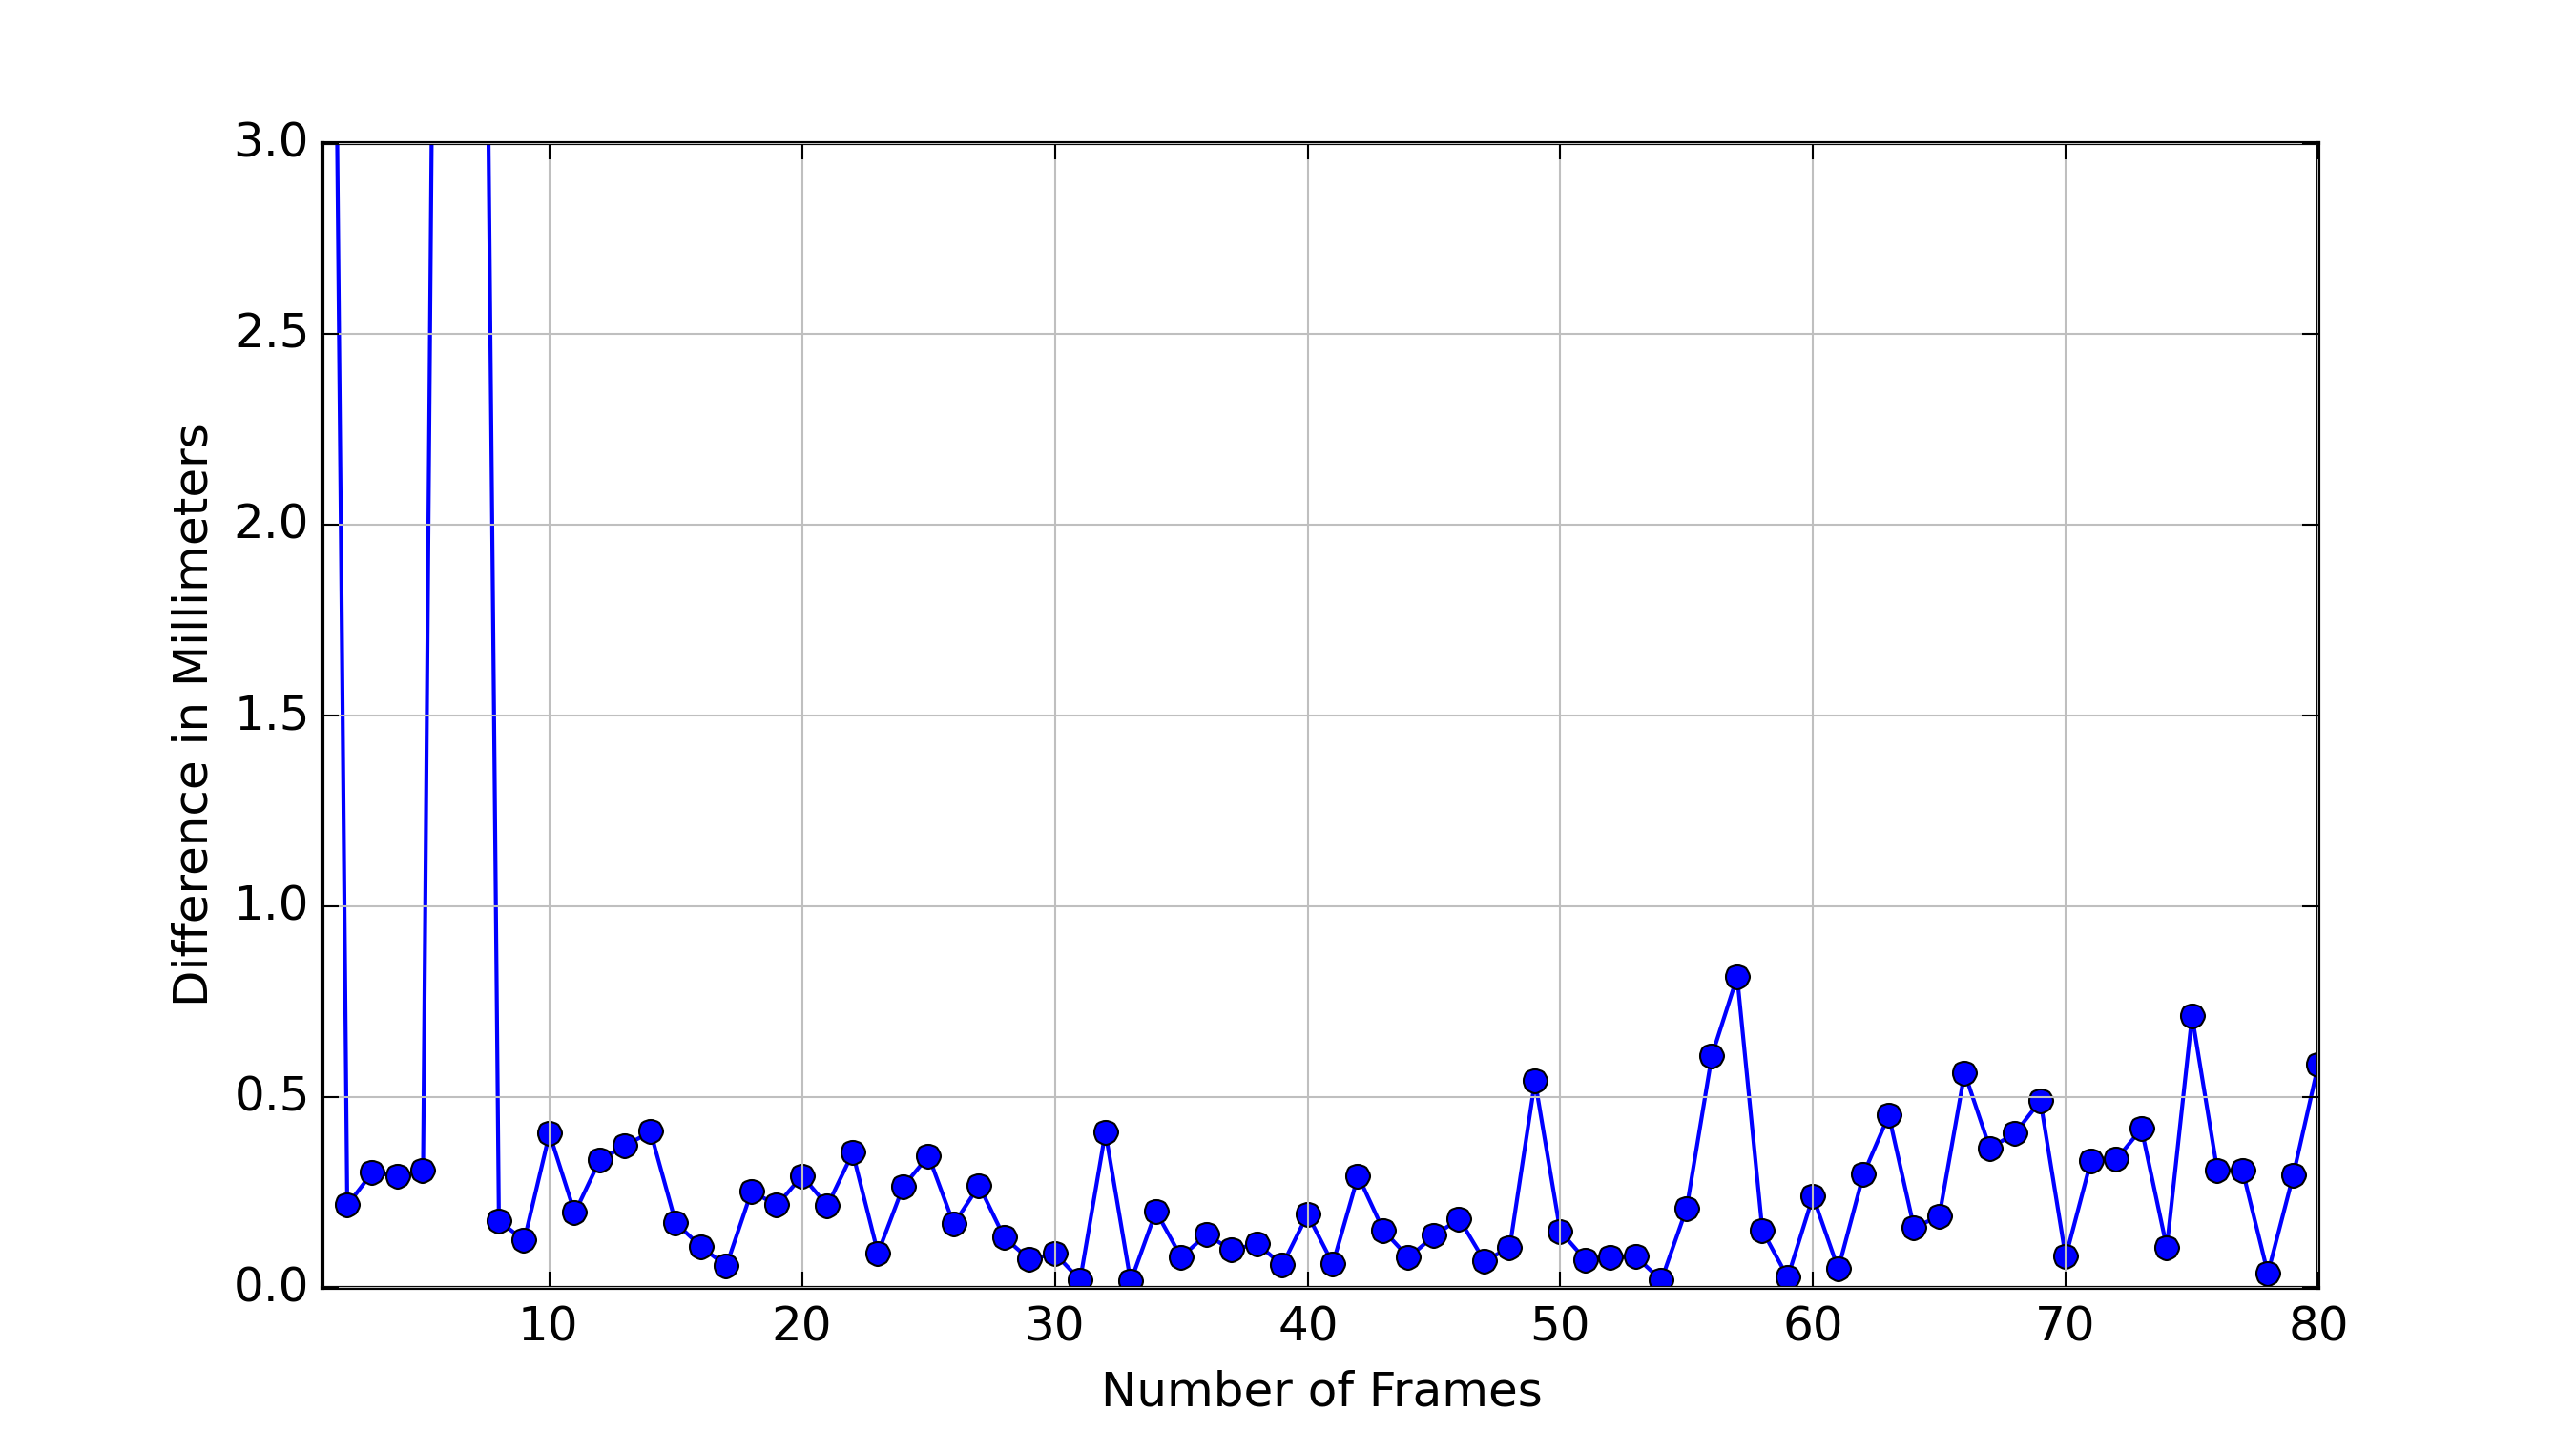
\includegraphics[width=80mm]{figures/diff_0/graph_translation} &  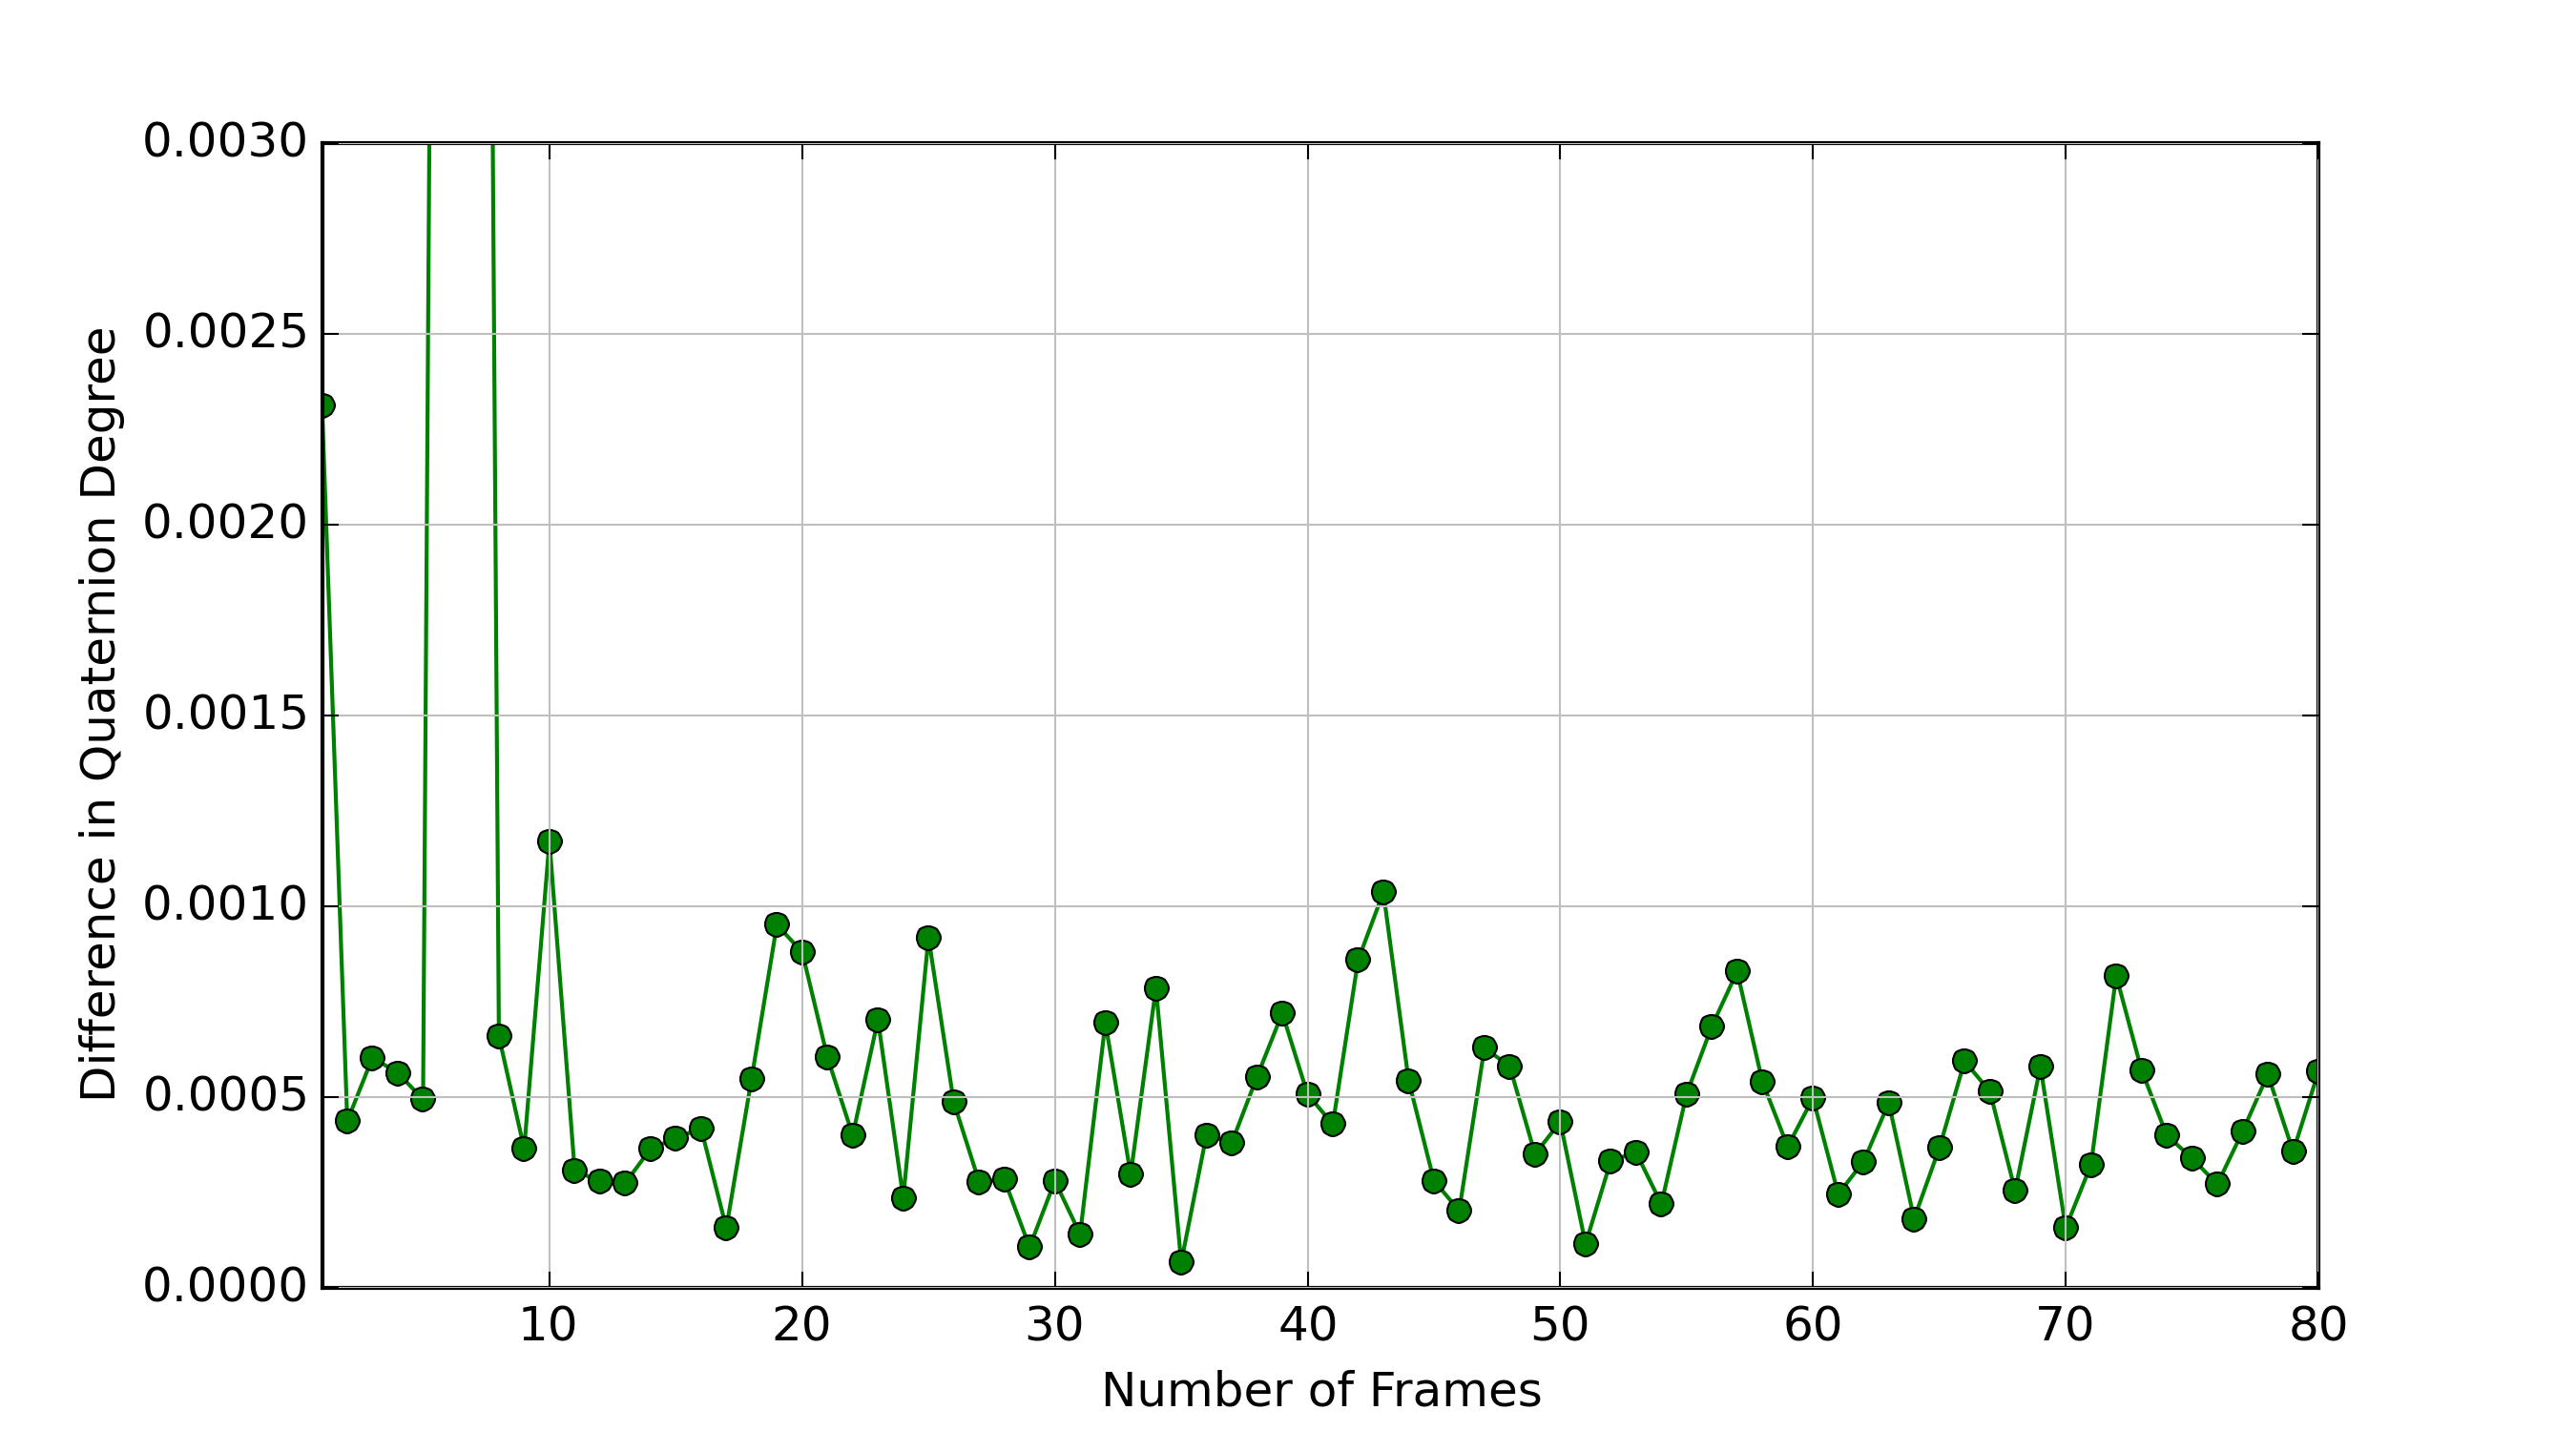
\includegraphics[width=80mm]{figures/diff_0/graph_rotation} \\
(a) Difference of translation & (b) Difference of rotation \\[6pt]
\end{tabular}
\caption{The movement of camera (difference of camera in time stamp $t$ and $t+1$) between the Feature-based and Marker-based for each sequence image pair of the first sample data set}\label{fig:sample_01_diff}
\end{figure}

\begin{table}[H]
\centering
  \begin{tabular}{| c | c | c | c |}
      \hline
      \multicolumn{2}{|c|}{Translation} & \multicolumn{2}{c|}{Rotation} \\ \hline
       Mean & Standard Deviation & Mean & Standard Deviation \\ \hline
      0.5089 & 1.3985 & 0.0007 & 0.0016 \\ \hline
  \end{tabular}
  \caption{} \label{tab:sample_01_diff}
\end{table}

Based on the \autoref{tab:sample_01_diff}, you can see that the change of rotation between each pair of images for both methods are closely similar where their mean values are just 0.0007 and it show that the both methods work similarly. For the tracking part, the \autoref{fig:sample_01_diff}(a) illustrates that the difference of tracking between these two methods for the first ten images are very high whereas for the rest frames, they become steady around the 0.5 millimeters.

\section{Sample Data Set 2} \label{sec:sample_2}
\begin{figure}[H]
\begin{tabular}{cc}
  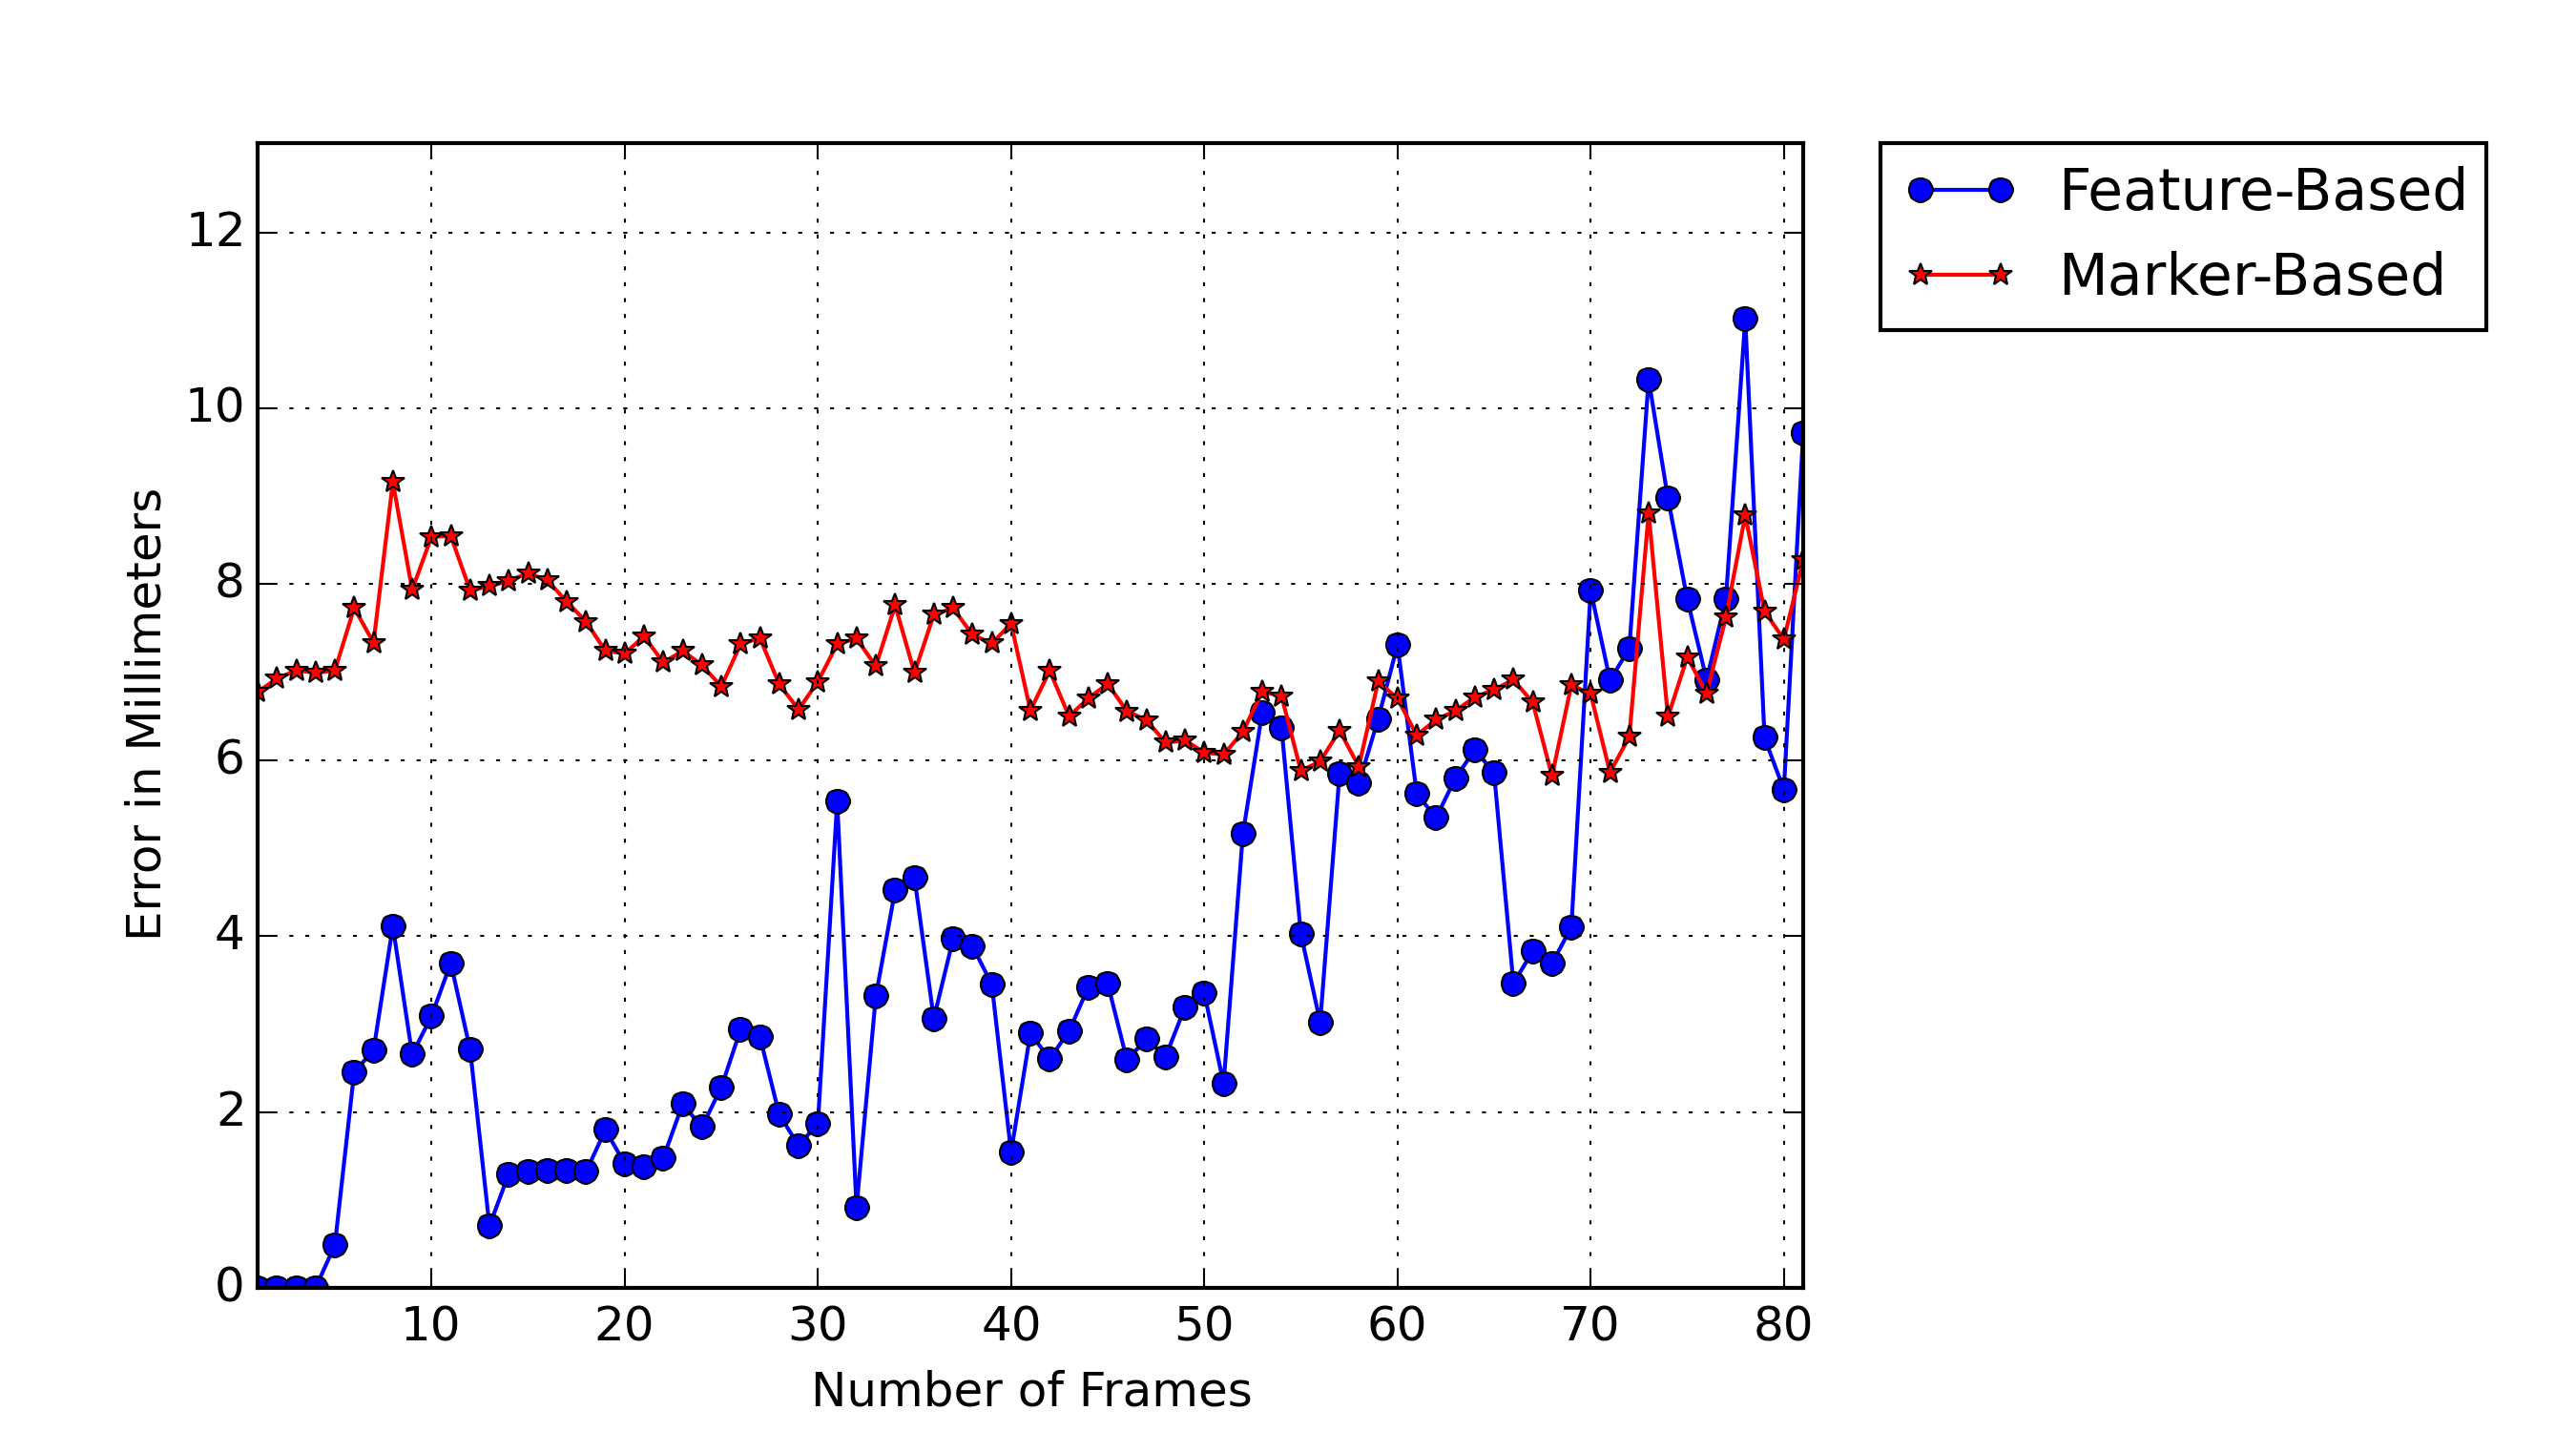
\includegraphics[width=80mm]{figures/frame_400/graph_translation} &  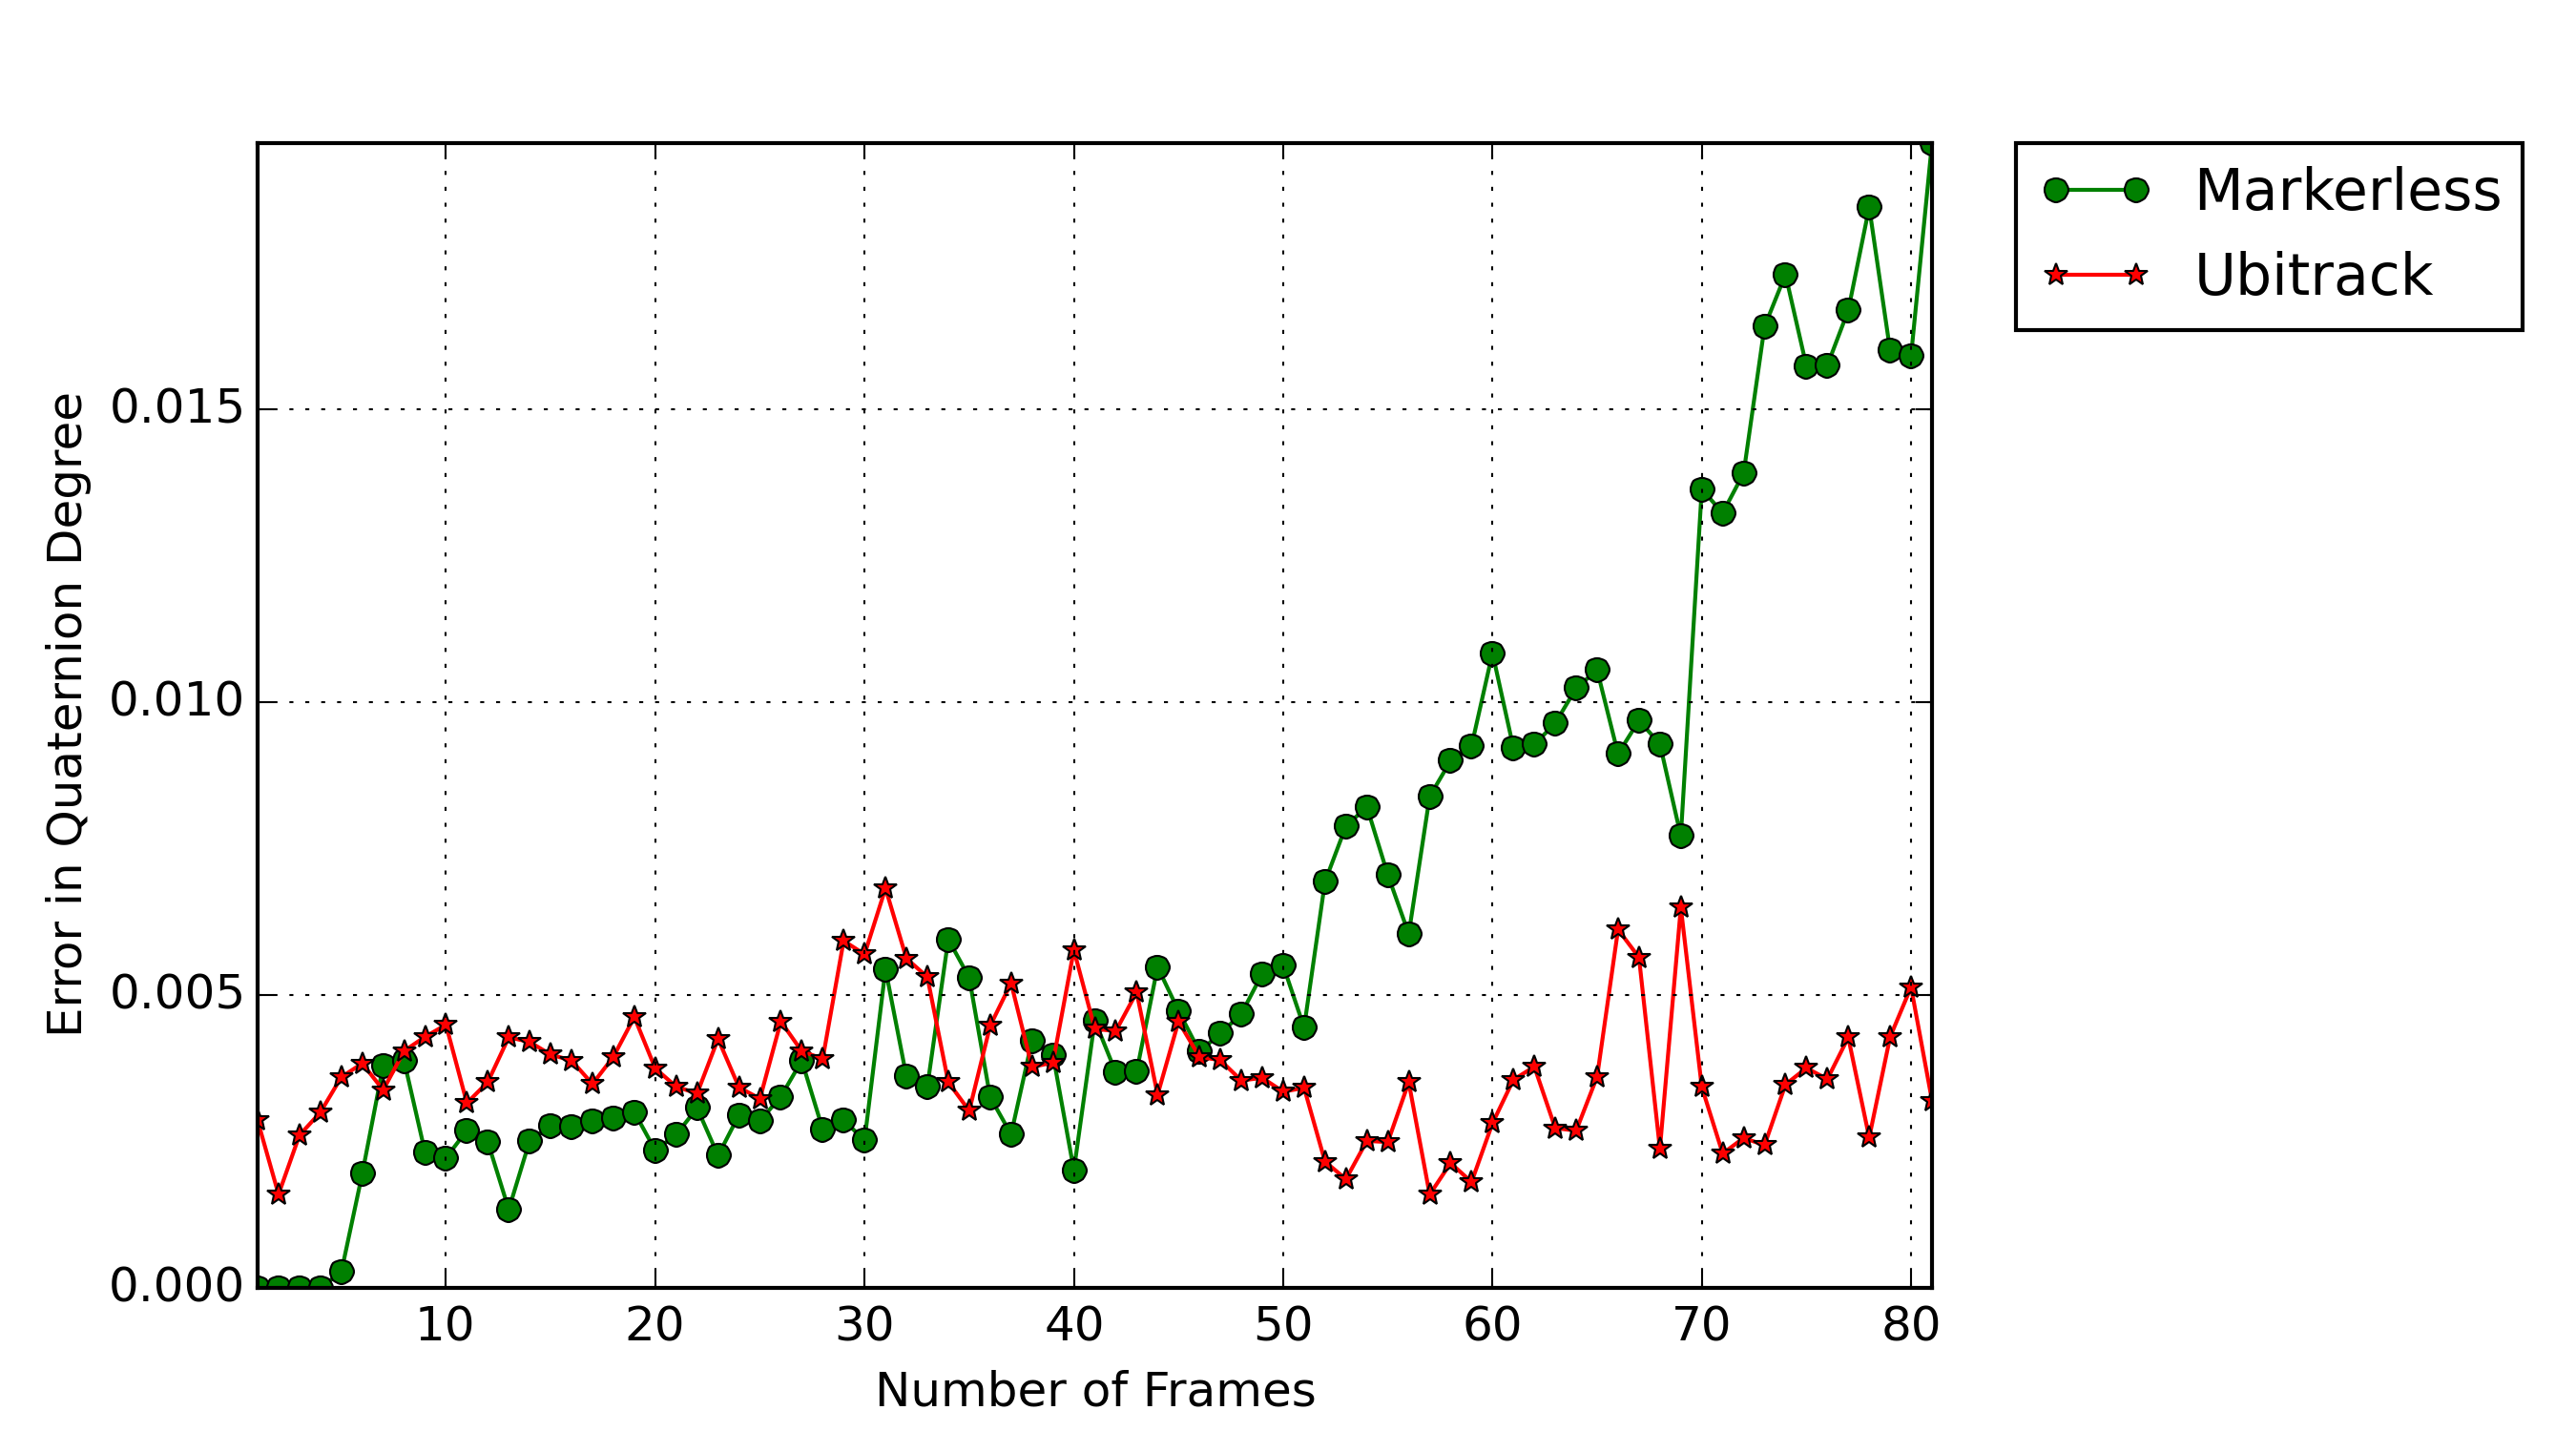
\includegraphics[width=80mm]{figures/frame_400/graph_rotation} \\
(a) the translation error in millimeters & (b) the rotation error in quaternion degree \\[6pt]
\end{tabular}
\caption{The tracking errors for both techniques based on the second ground truth data set}\label{fig:sample_02}
\end{figure}

\begin{table}[H]
\centering
  \begin{tabular}{| c || c | c | c | c |}
      \hline
      & \multicolumn{2}{c|}{Translation} & \multicolumn{2}{c|}{Rotation} \\ \hline
       & Mean & Standard Deviation & Mean & Standard Deviation \\ \hline
      Feature-Based Approach & 3.8357 & 2.4783 & 0.0063 & 0.0049 \\ \hline
      Marker-Based Approach & 7.0932 & 0.7227 & 0.0037 & 0.0011 \\ \hline
  \end{tabular}
  \caption{The statistical analysis of tracking error for both methods based on the second ground truth data set} \label{tab:sample_02}
\end{table}

\autoref{tab:sample_02} and \autoref{fig:sample_02} show the result of comparison of translation and rotation errors with the ground truth for the second sample data set. The result of rotation column of \autoref{tab:sample_02} and \autoref{fig:sample_02}(b) represent a very important event in this master thesis. They show that for some data sets, the rotation estimation and optimization does not work as well as the translation estimation. 
It might be the result of two things: observing a huge rotation that our pose estimation and PnP solver can not handle it or bad estimation for the rotation of one frame that has a cumulative error on our estimated rotation and has a bad effect on our both local and global bundle adjustment. \autoref{fig:sample_02} also shows that the translation and rotation have a reflective effect on each other. It means when we have a fast increase in the error rate of rotation, it consequently has a negative effect on estimating the translation. In details, the average of translation estimations error before the 50th frames is around 1.8 millimeters, but as the rotation estimation gets worse, the translation error increases 4 four millimeters to 10 millimeters.

\begin{figure}[H]
\begin{tabular}{cc}
  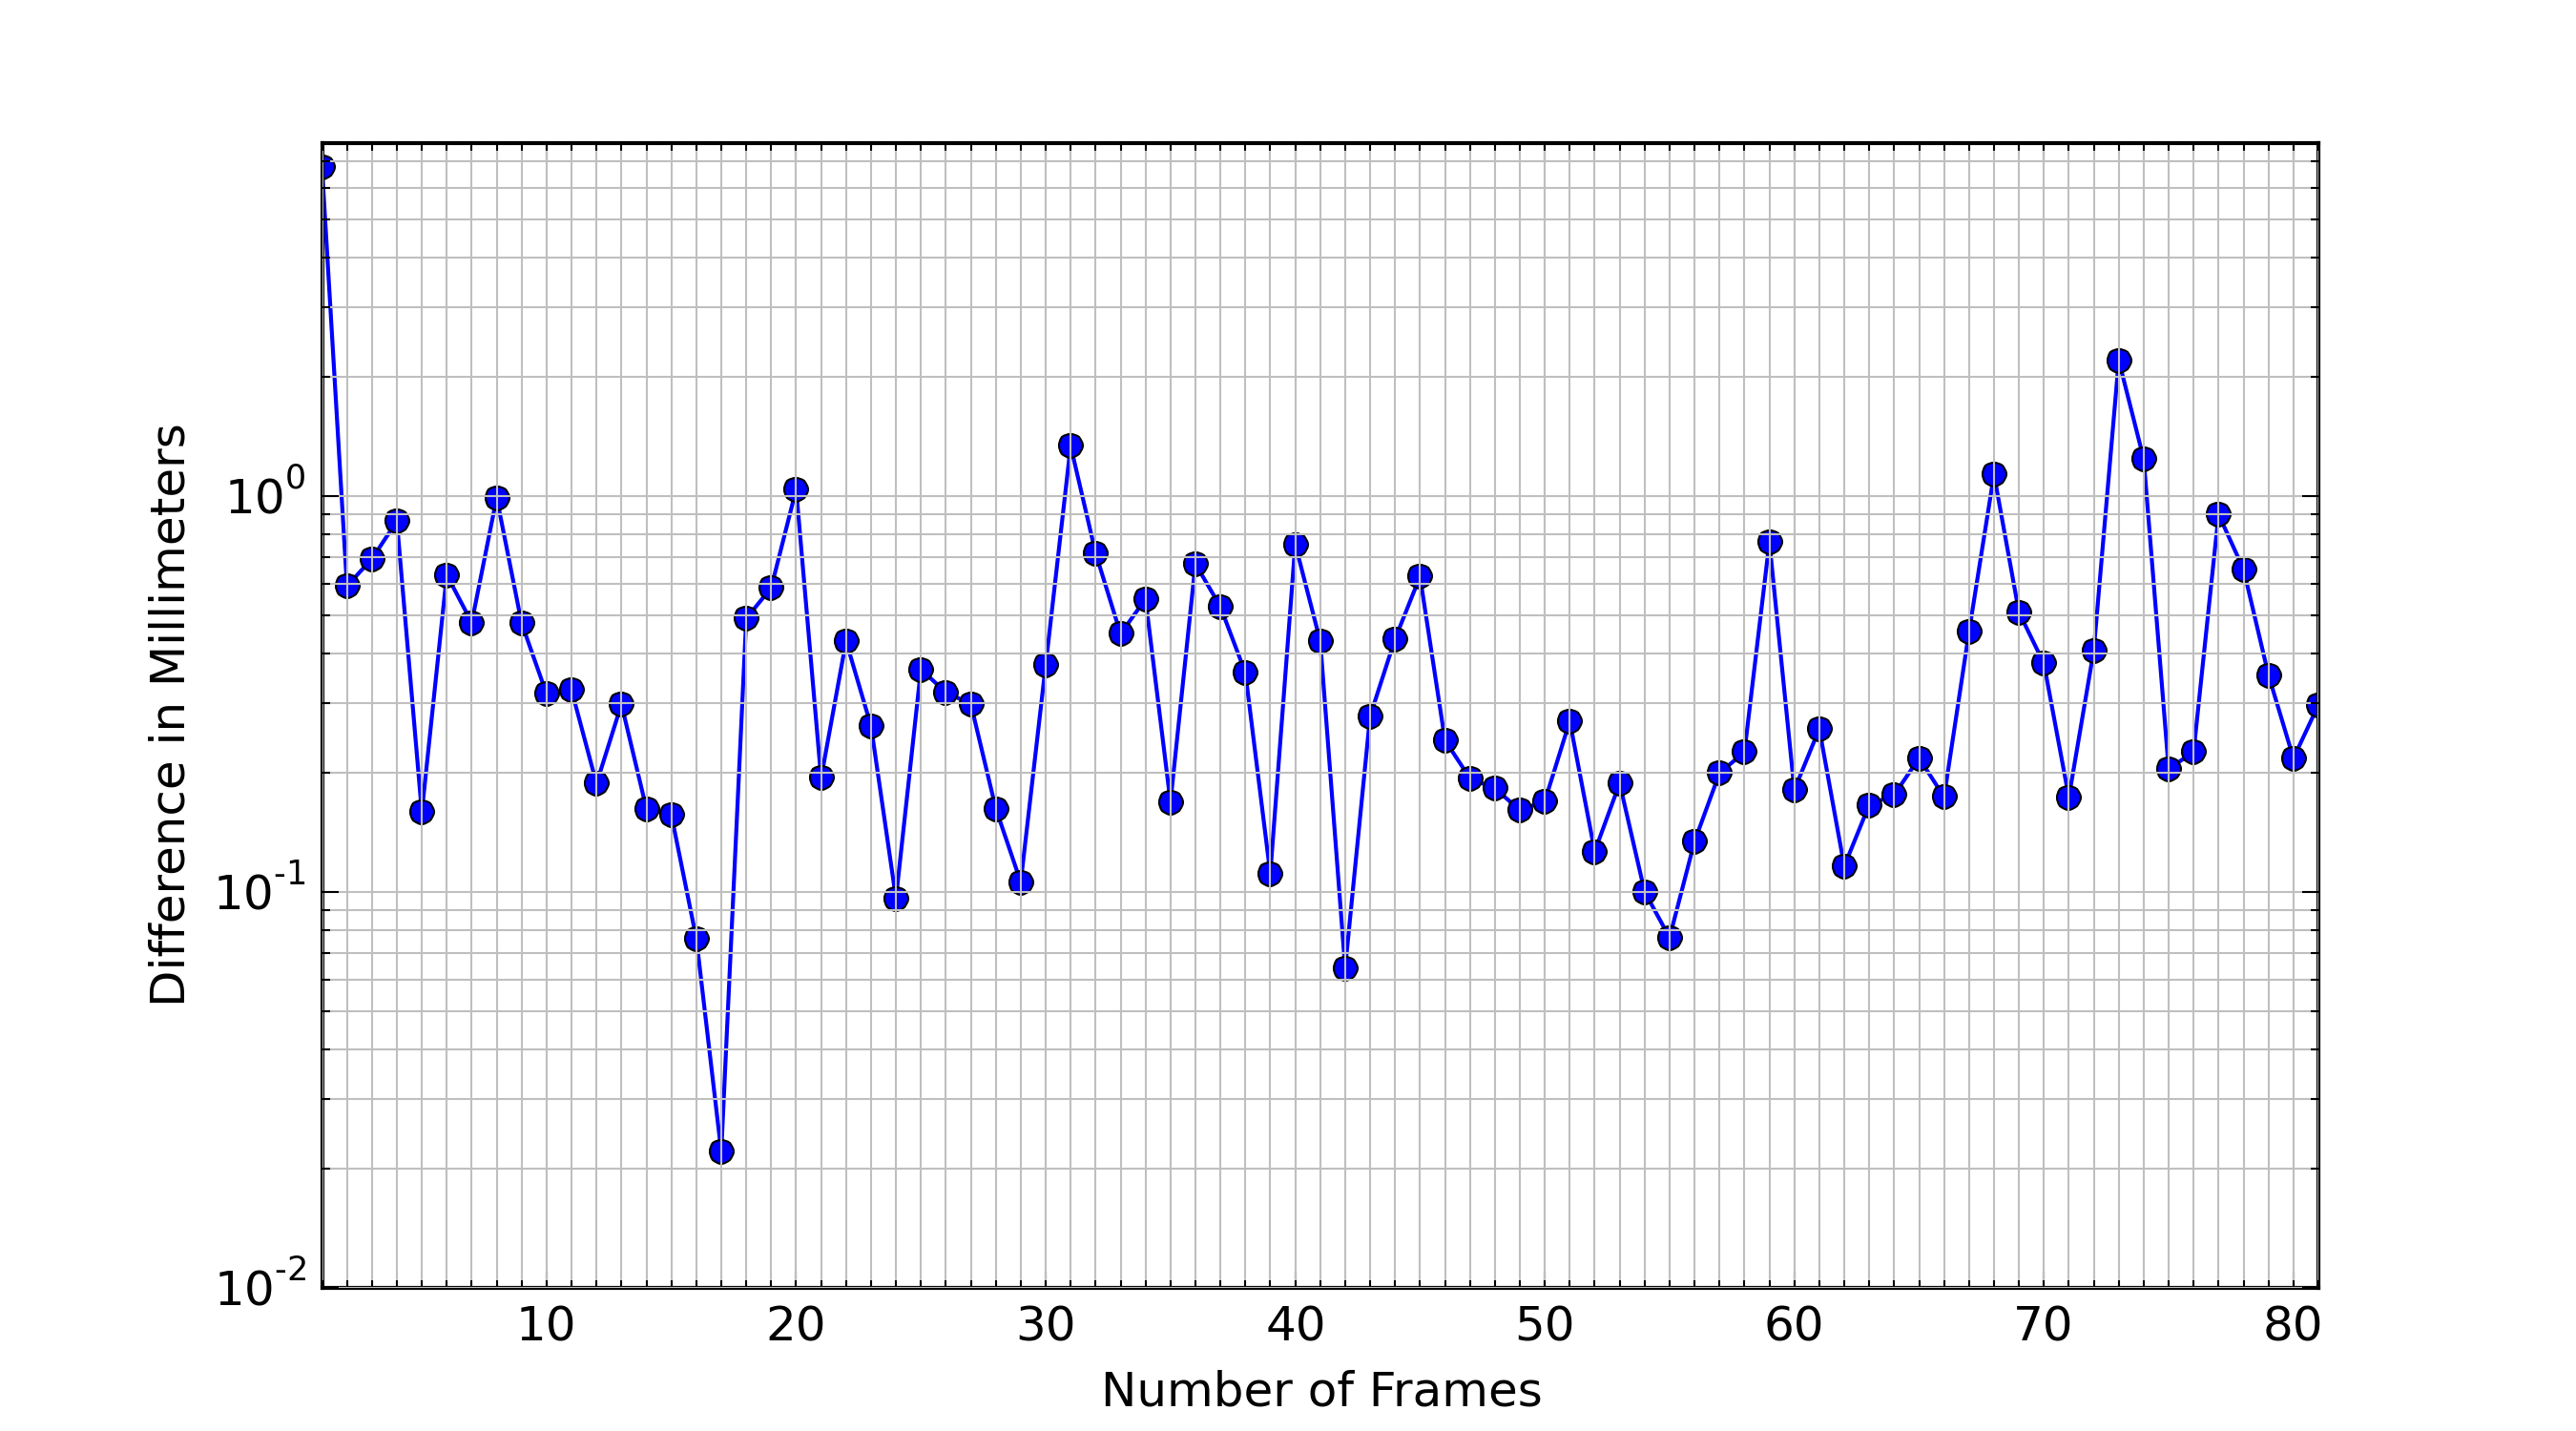
\includegraphics[width=80mm]{figures/diff_400/graph_translation} &  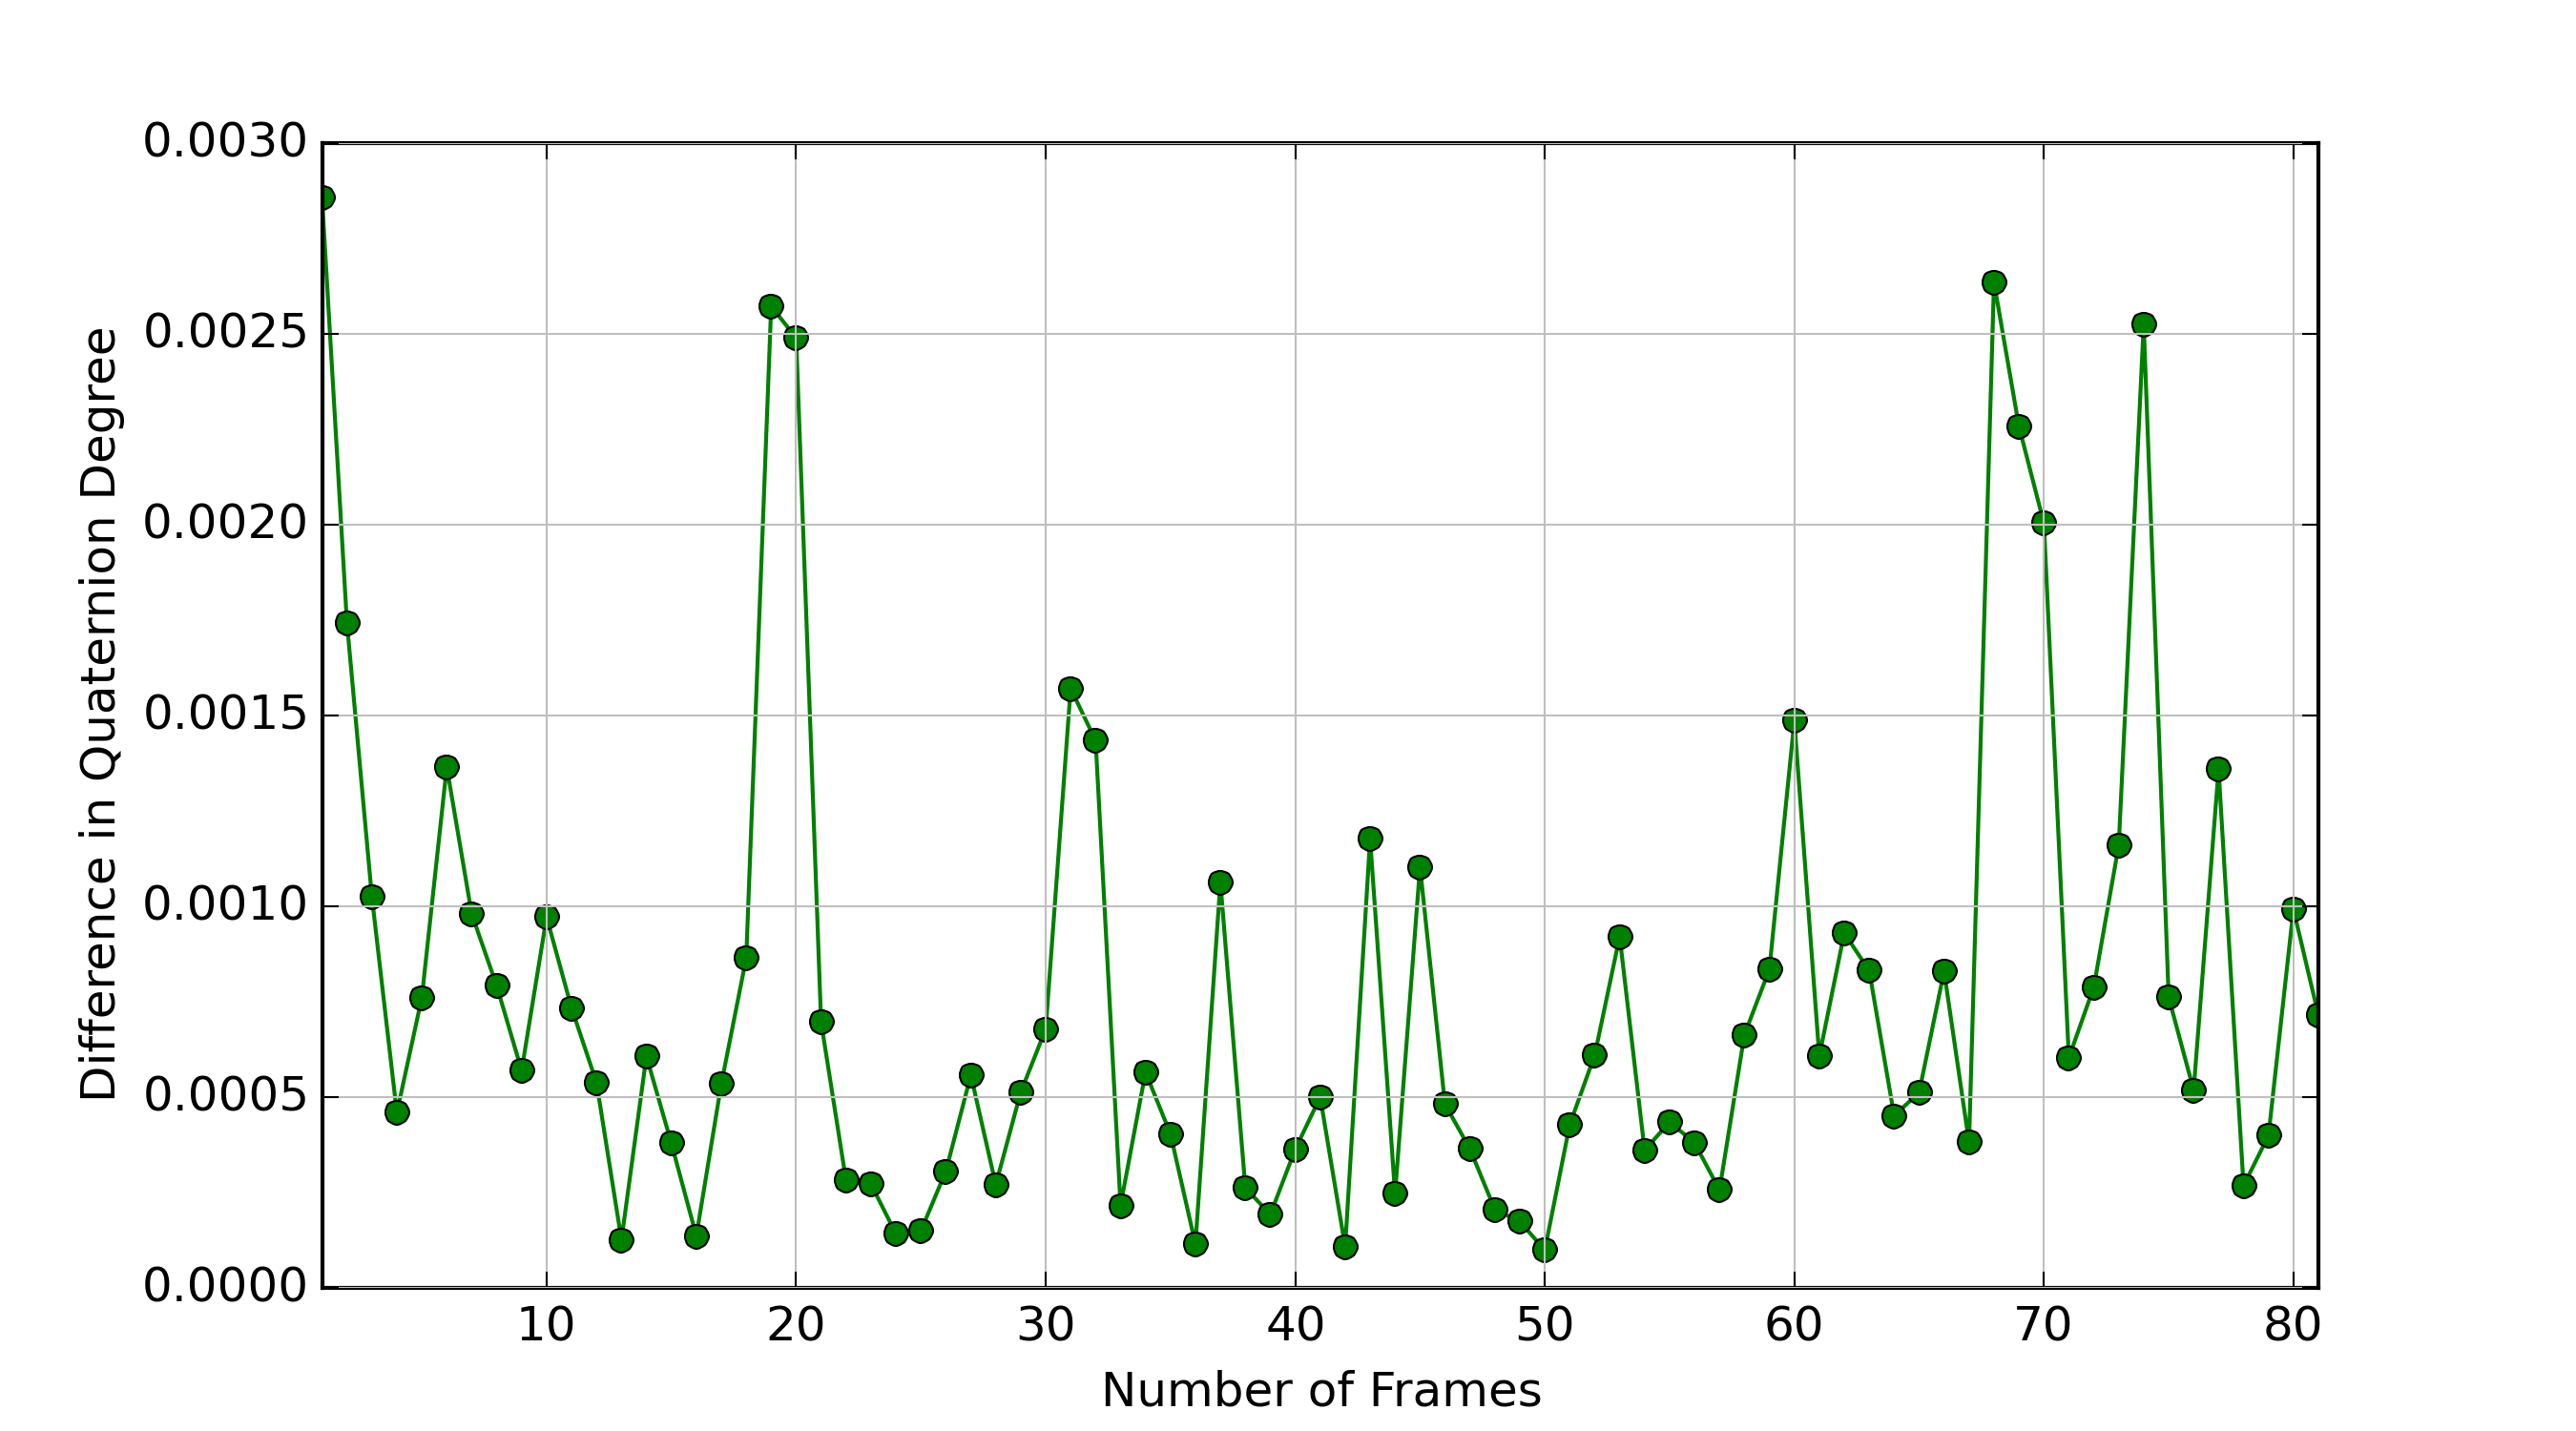
\includegraphics[width=80mm]{figures/diff_400/graph_rotation} \\
(a) difference of translation in milliliters & (b) difference of rotation in degree of quaternion \\[6pt]
\end{tabular}
\caption{The difference between the Feature-based and Marker-based for each sequence pair of second sample data set}\label{fig:sample_02_diff}
\end{figure}

\begin{table}[H]
\centering
  \begin{tabular}{| c | c | c | c |}
      \hline
      \multicolumn{2}{|c|}{Translation} & \multicolumn{2}{c}{Rotation} \\ \hline
       Mean & Standard Deviation & Mean & Standard Deviation \\ \hline
      0.4821 & 0.7839 & 0.0008 & 0.0006 \\ \hline
  \end{tabular}
  \caption{} \label{tab:sample_02_diff}
\end{table}

The \autoref{tab:sample_02_diff} represent a comparison of difference of camera (both rotation and translation) for both marker-based and feature-based methods. However the general trend for both methods of the first data set (see \autoref{tab:sample_01_diff}) was stable, while the results of the second data set have a fluctuation trends. For instance in \nth{20}, \nth{31} and \nth{73} frames, we can see a huge zig-zag pattern in both translation and rotation graphs. These problems in estimating the rotation and translation can be caused by the huge error that we have in estimating the rotation. 

\section{Sample Data Set 3} \label{subsec:sample_3}
\begin{figure}[H]
\begin{tabular}{cc}
  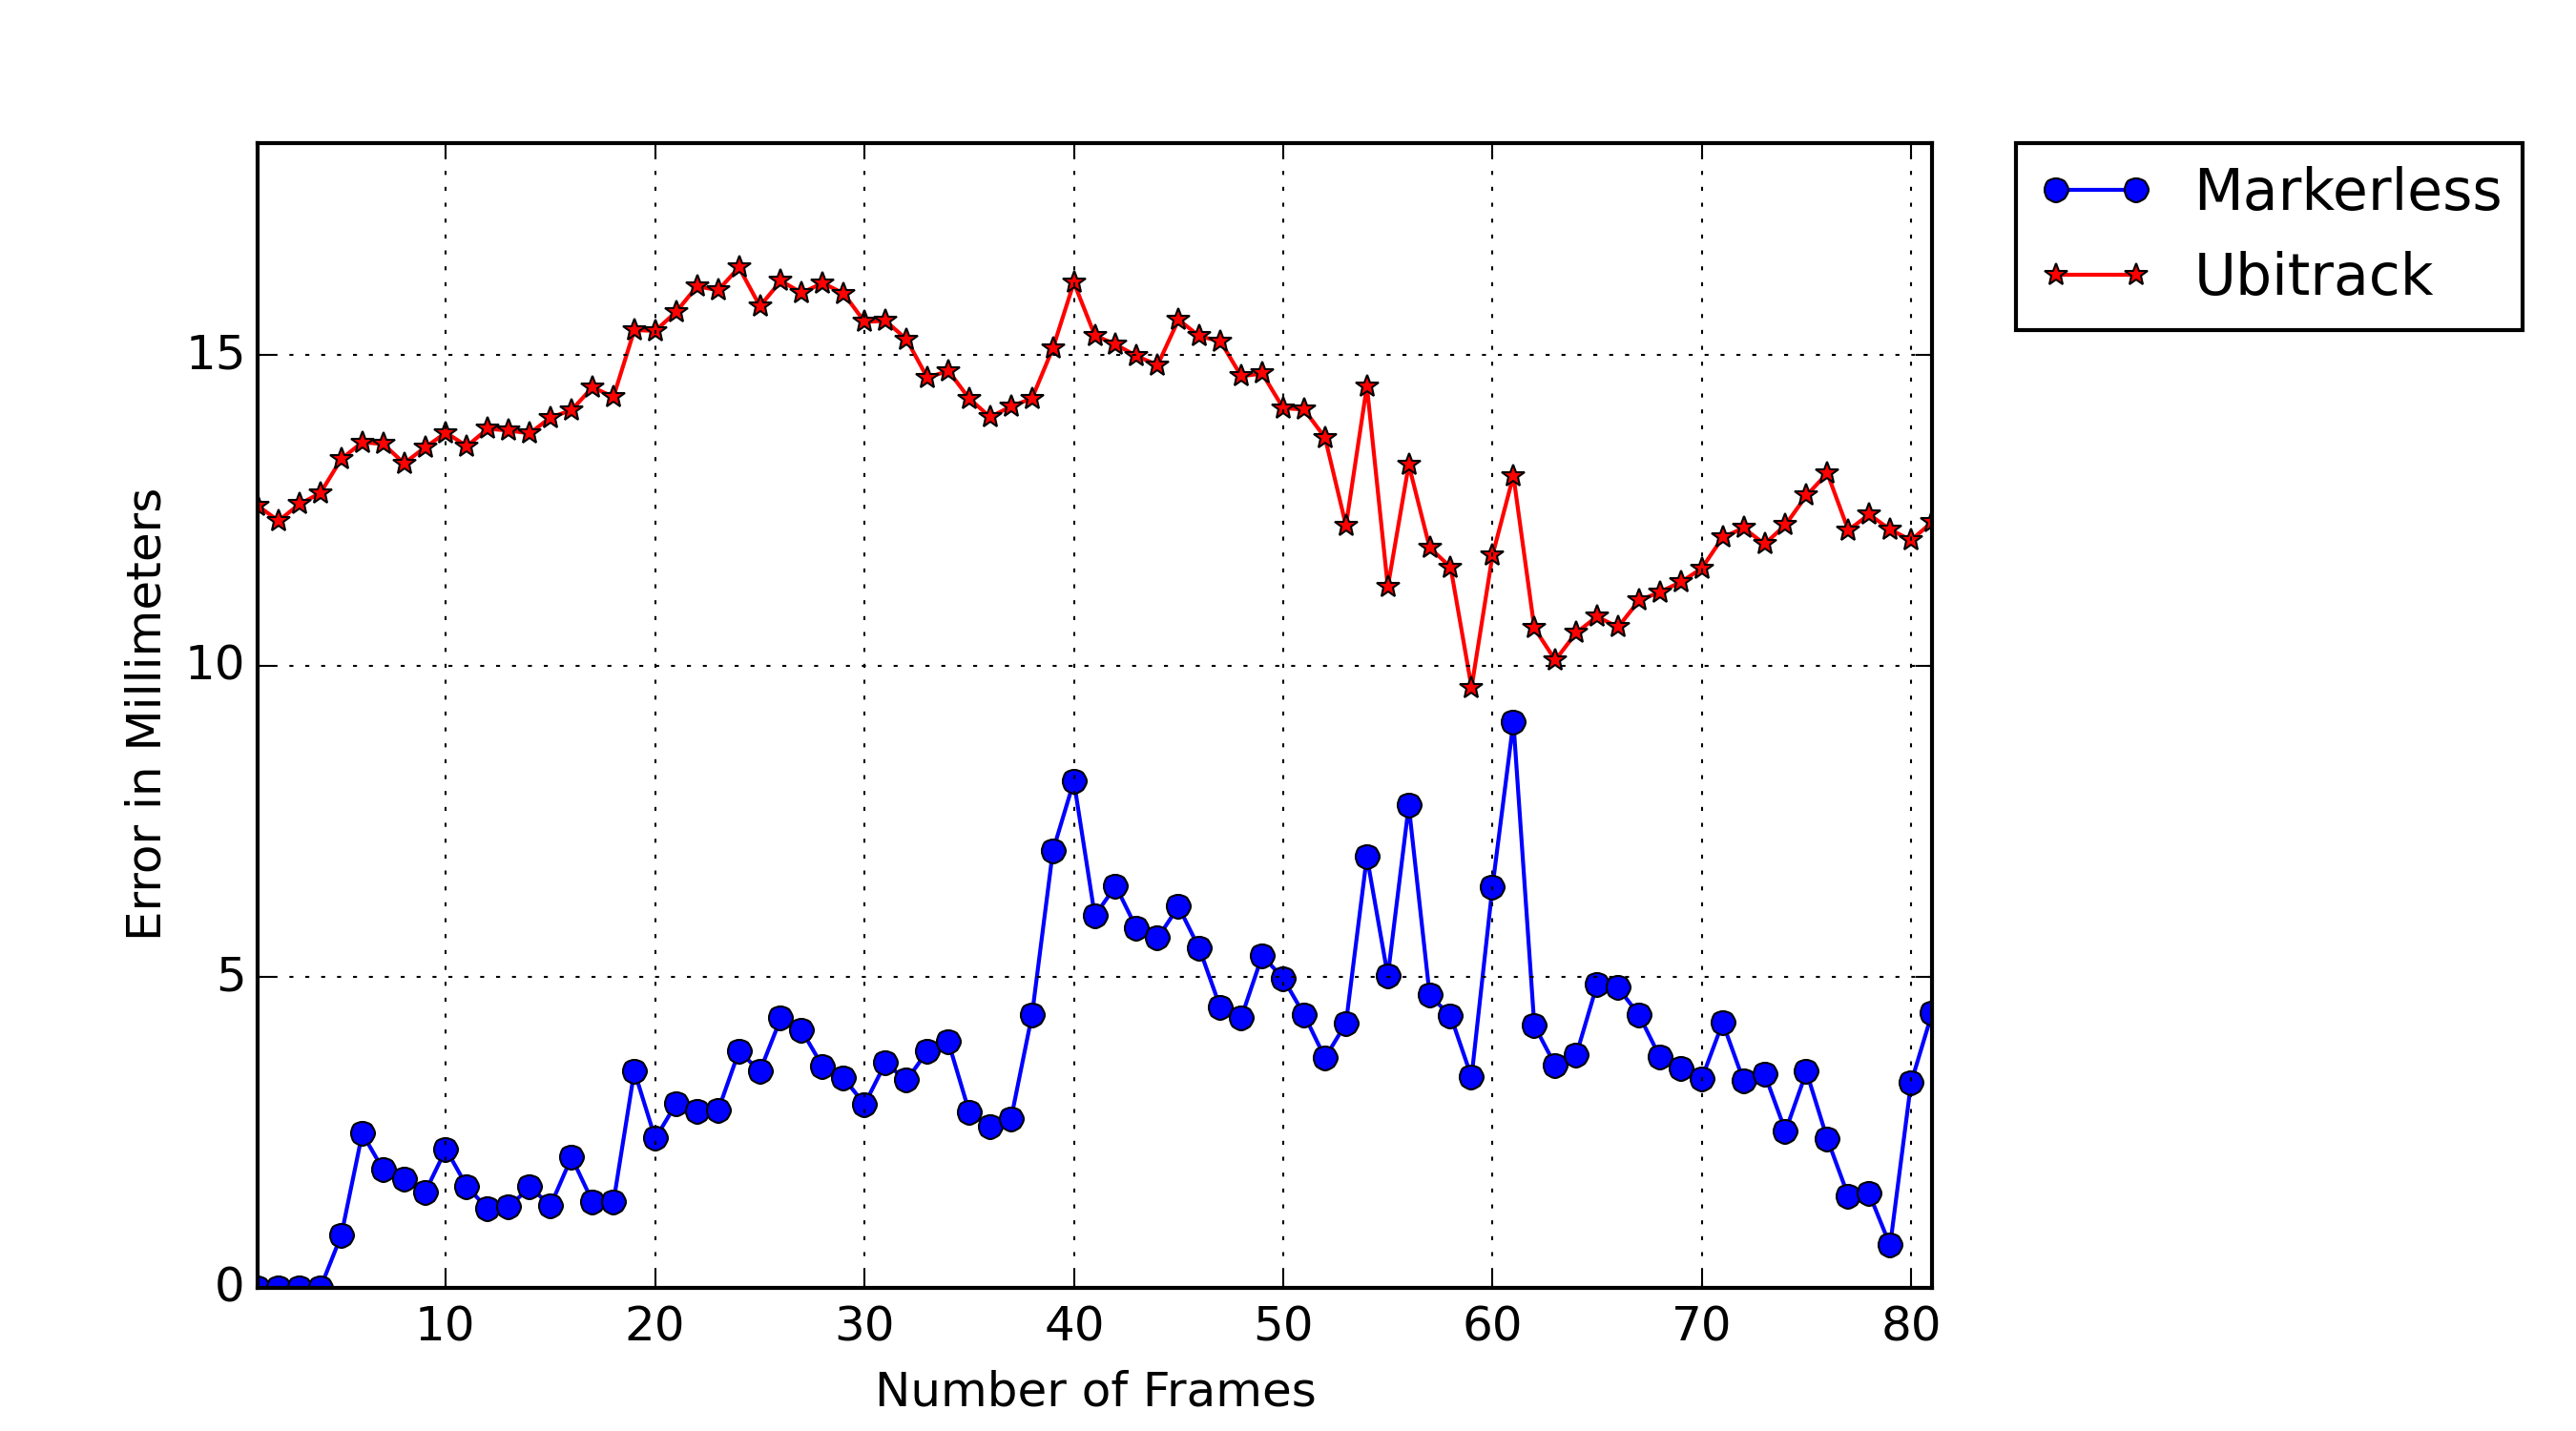
\includegraphics[width=80mm]{figures/frame_600/graph_translation} &  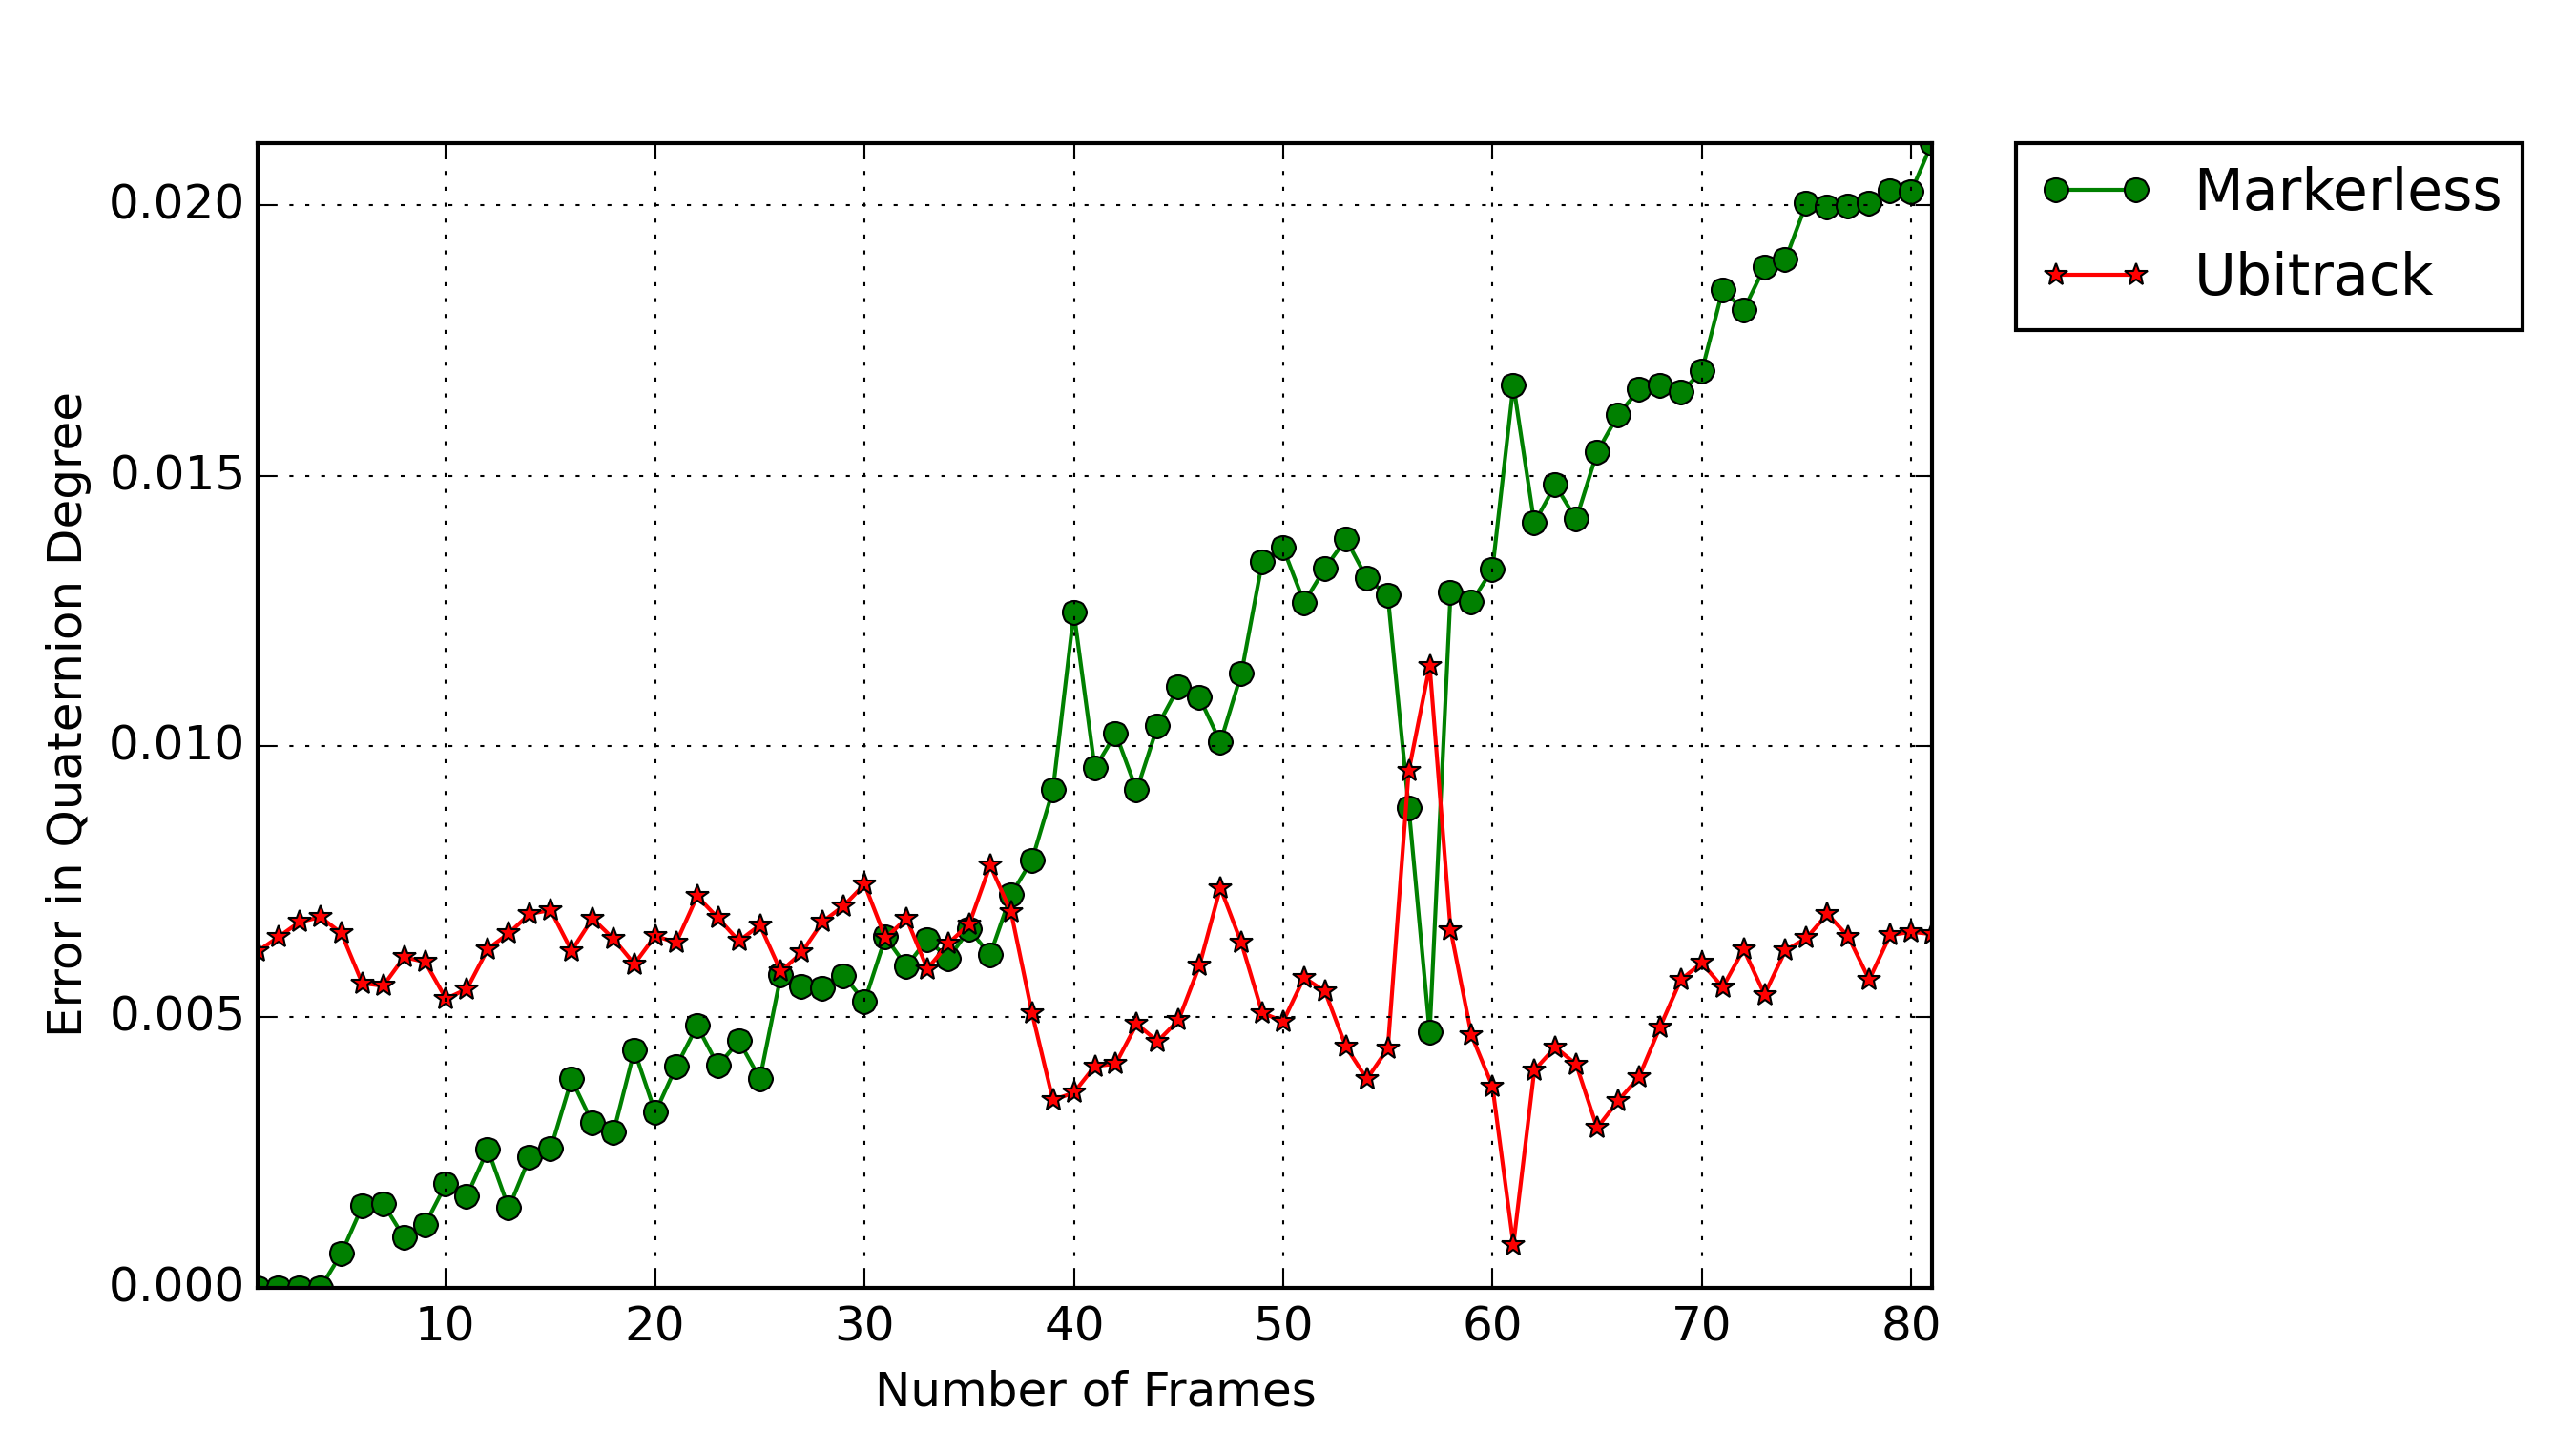
\includegraphics[width=80mm]{figures/frame_600/graph_rotation} \\
(a) translation & (b) rotation \\[6pt]
\end{tabular}
\caption{The tracking errors for both feature-based and marker-based techniques based on the third ground truth data set}\label{fig:sample_03}
\end{figure}

\begin{table}[H]
\centering
  \begin{tabular}{| c || c | c | c | c |}
      \hline
      & \multicolumn{2}{c|}{Translation} & \multicolumn{2}{c|}{Rotation} \\ \hline
       & Mean & Standard Deviation & Mean & Standard Deviation \\ \hline
      Feature-Based Approach & 3.5443 & 1.8751 & 0.0094 & 0.0063 \\ \hline
      Marker-Base Approach & 13.6084 & 1.6970 & 0.0058 & 0.0014 \\ \hline
  \end{tabular}
  \caption{the statistical analysis of tracking error for both feature-based and marker-based techniques based on the second ground truth data set} \label{tab:sample_03}
\end{table}

\autoref{tab:sample_03} and \autoref{fig:sample_03} show the result of comparison of translation and rotation errors with the ground truth for the third sample data set. These results prove that our idea about the replacing of 3D points in world map with the new one after each 35 frames was true. Let me to divide the \autoref{fig:sample_03}(a) into 3 parts. for the first seven bundles (frames 1 to 35), second seven bundles (from 36 to 70) and the rest. As you can see in \autoref{fig:sample_03}, the translation error in the first part (first seven bundles) is around the 2.5 millimeters. After that the inefficient results of the rotation that has a dramatical growth, cause the translation estimations also have a jump to the up and the mean of error is set around the 5.5 millimeters. But after the 70th frame and because the whole 3D points in world map are replaced with the new data, the local and global bundle adjustment could control the error of the translation for the next frames and bundles. In the case of rotation, once more is happened that rotation estimation and optimization are not efficient as well as the translation part.

\begin{figure}[H]
\begin{tabular}{cc}
  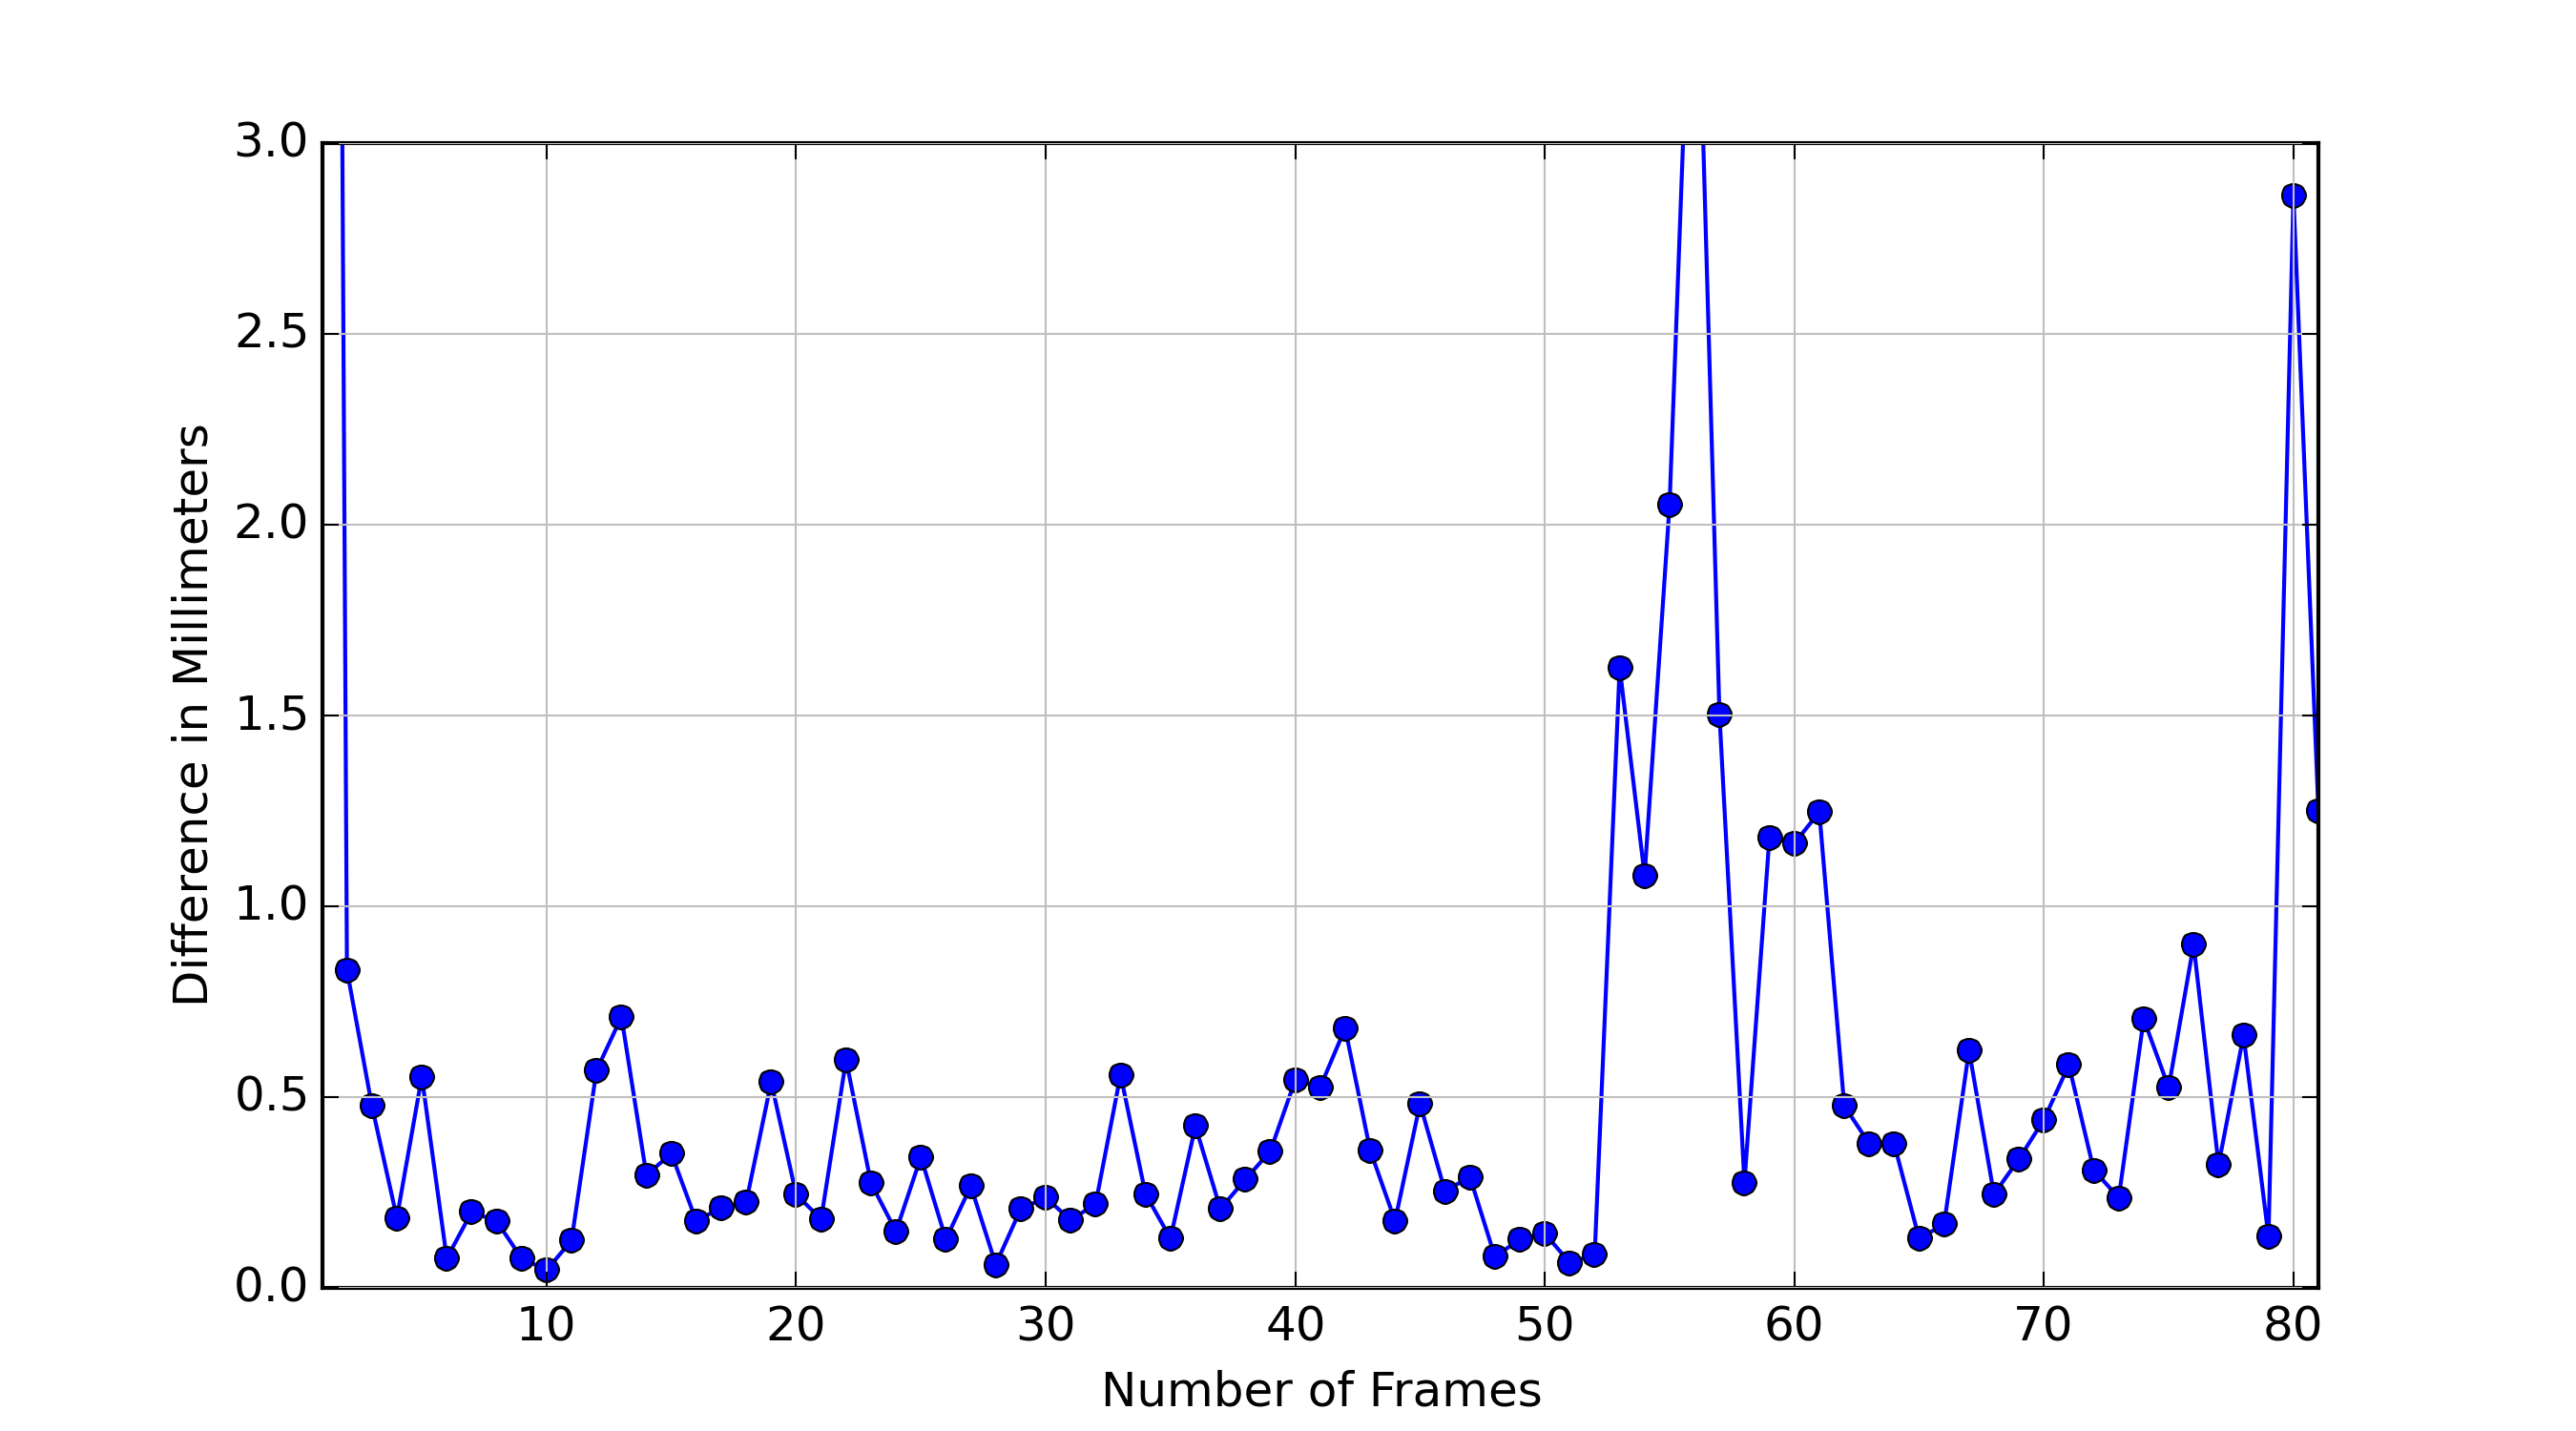
\includegraphics[width=80mm]{figures/diff_600/graph_translation} &  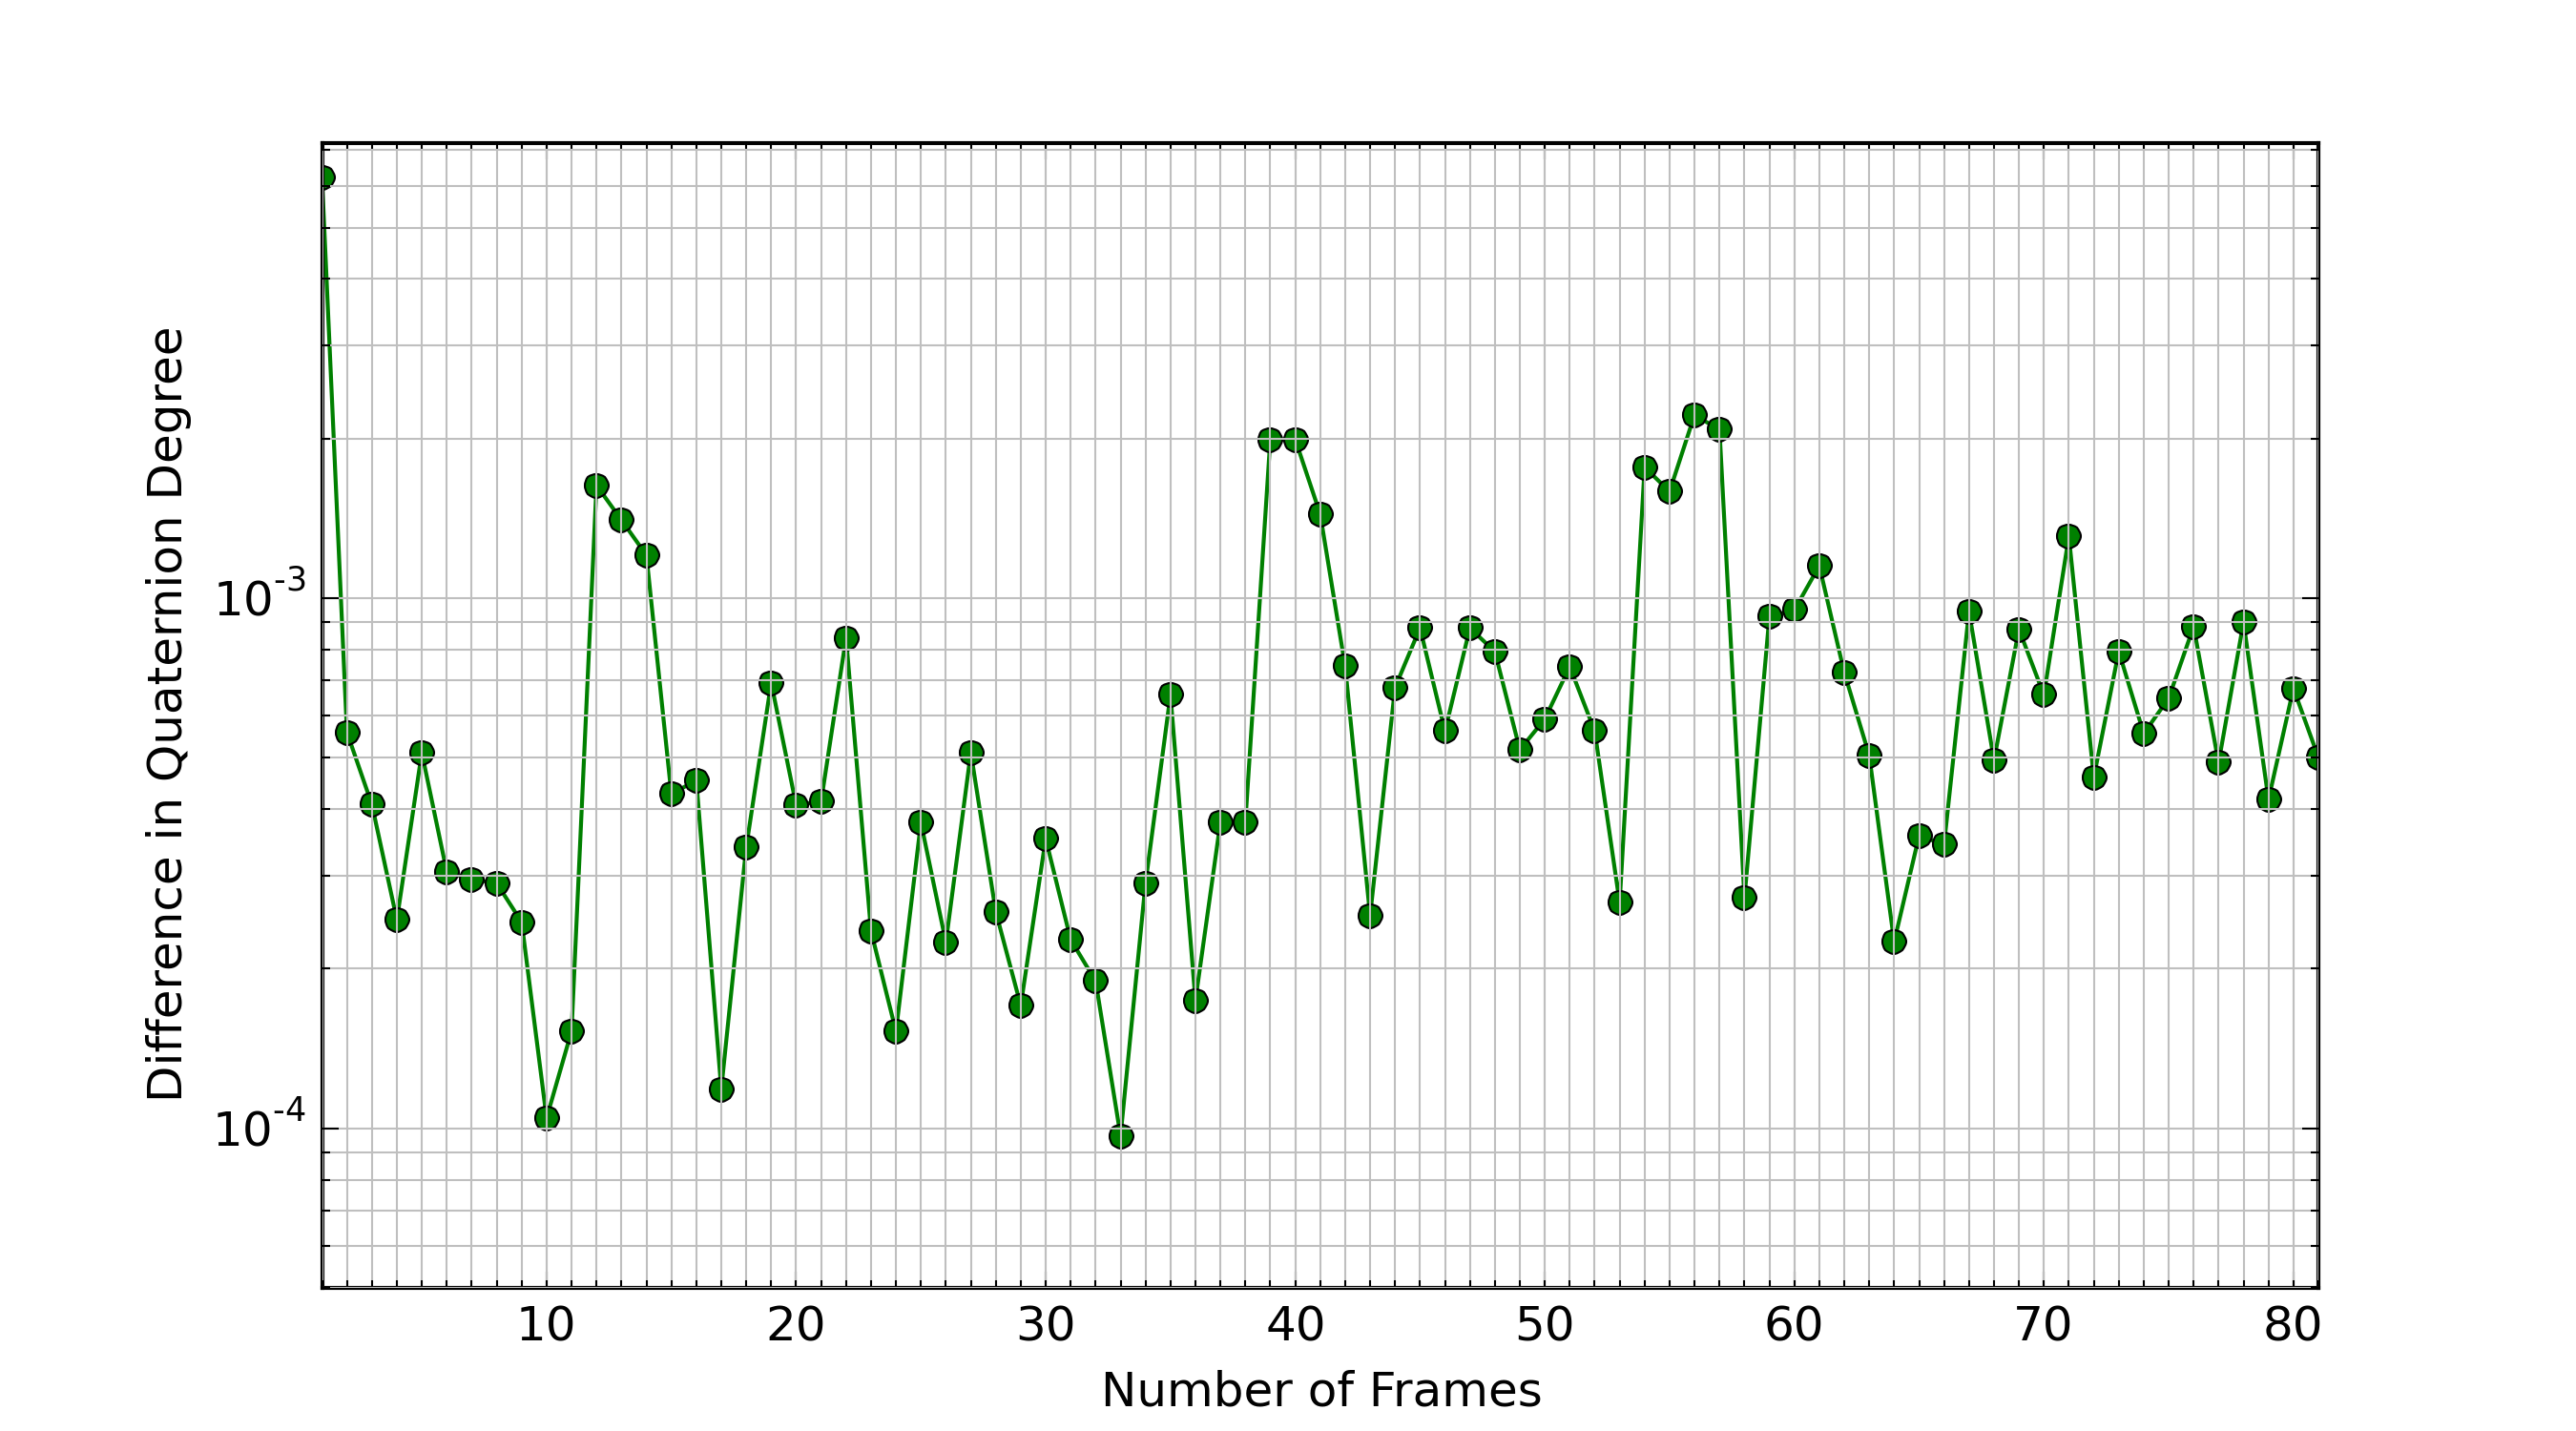
\includegraphics[width=80mm]{figures/diff_600/graph_rotation} \\
(a) Difference of translation & (b) Difference of rotation \\[6pt]
\end{tabular}
\caption{The difference between the Feature-based and Marker-based for each sequence pair of third sample data set}\label{fig:sample_03_diff}
\end{figure}

\begin{table}[H]
\centering
  \begin{tabular}{| c | c | c | c |}
      \hline
      \multicolumn{2}{|c|}{Translation} & \multicolumn{2}{c}{Rotation} \\ \hline
       Mean & Standard Deviation & Mean & Standard Deviation \\ \hline
      0.6558 & 1.4589 & 0.0007 & 0.0008 \\ \hline
  \end{tabular}
  \caption{} \label{tab:sample_03_diff}
\end{table}

\autoref{fig:sample_03_diff} and \autoref{tab:sample_03_diff} demonstrate the difference of camera movement which computed by the feature-based and marker-based approaches. The trend of translation is steady around the 0.25 millimeters for the first fifty frames. But after that an extreme fluctuation pattern appears between the \nth{52} and \nth{65} frames. As we analyzed in previous tests, it can be caused by the error of rotation estimation. After The \nth{70} frame that the 3D world map is replaced with new 3D points, the error of rotation and translation decreases and consequently the similarity measure between the marker-based and feature-based approaches increases.

\section{Test local threshold} \label{sec:local_threshold}
In this test, we evaluate the performance of a parameter that describes the number of images in a bundle. This size is called local threshold (for more detail see \autoref{sebsec:bundle_concept}). In this test we run the first sample data set (\autoref{sec:sample_01}) for three times with the size of 3, 5, and 7 for a bundle.
\begin{figure}[H]
\centering
\begin{tabular}{cc}
  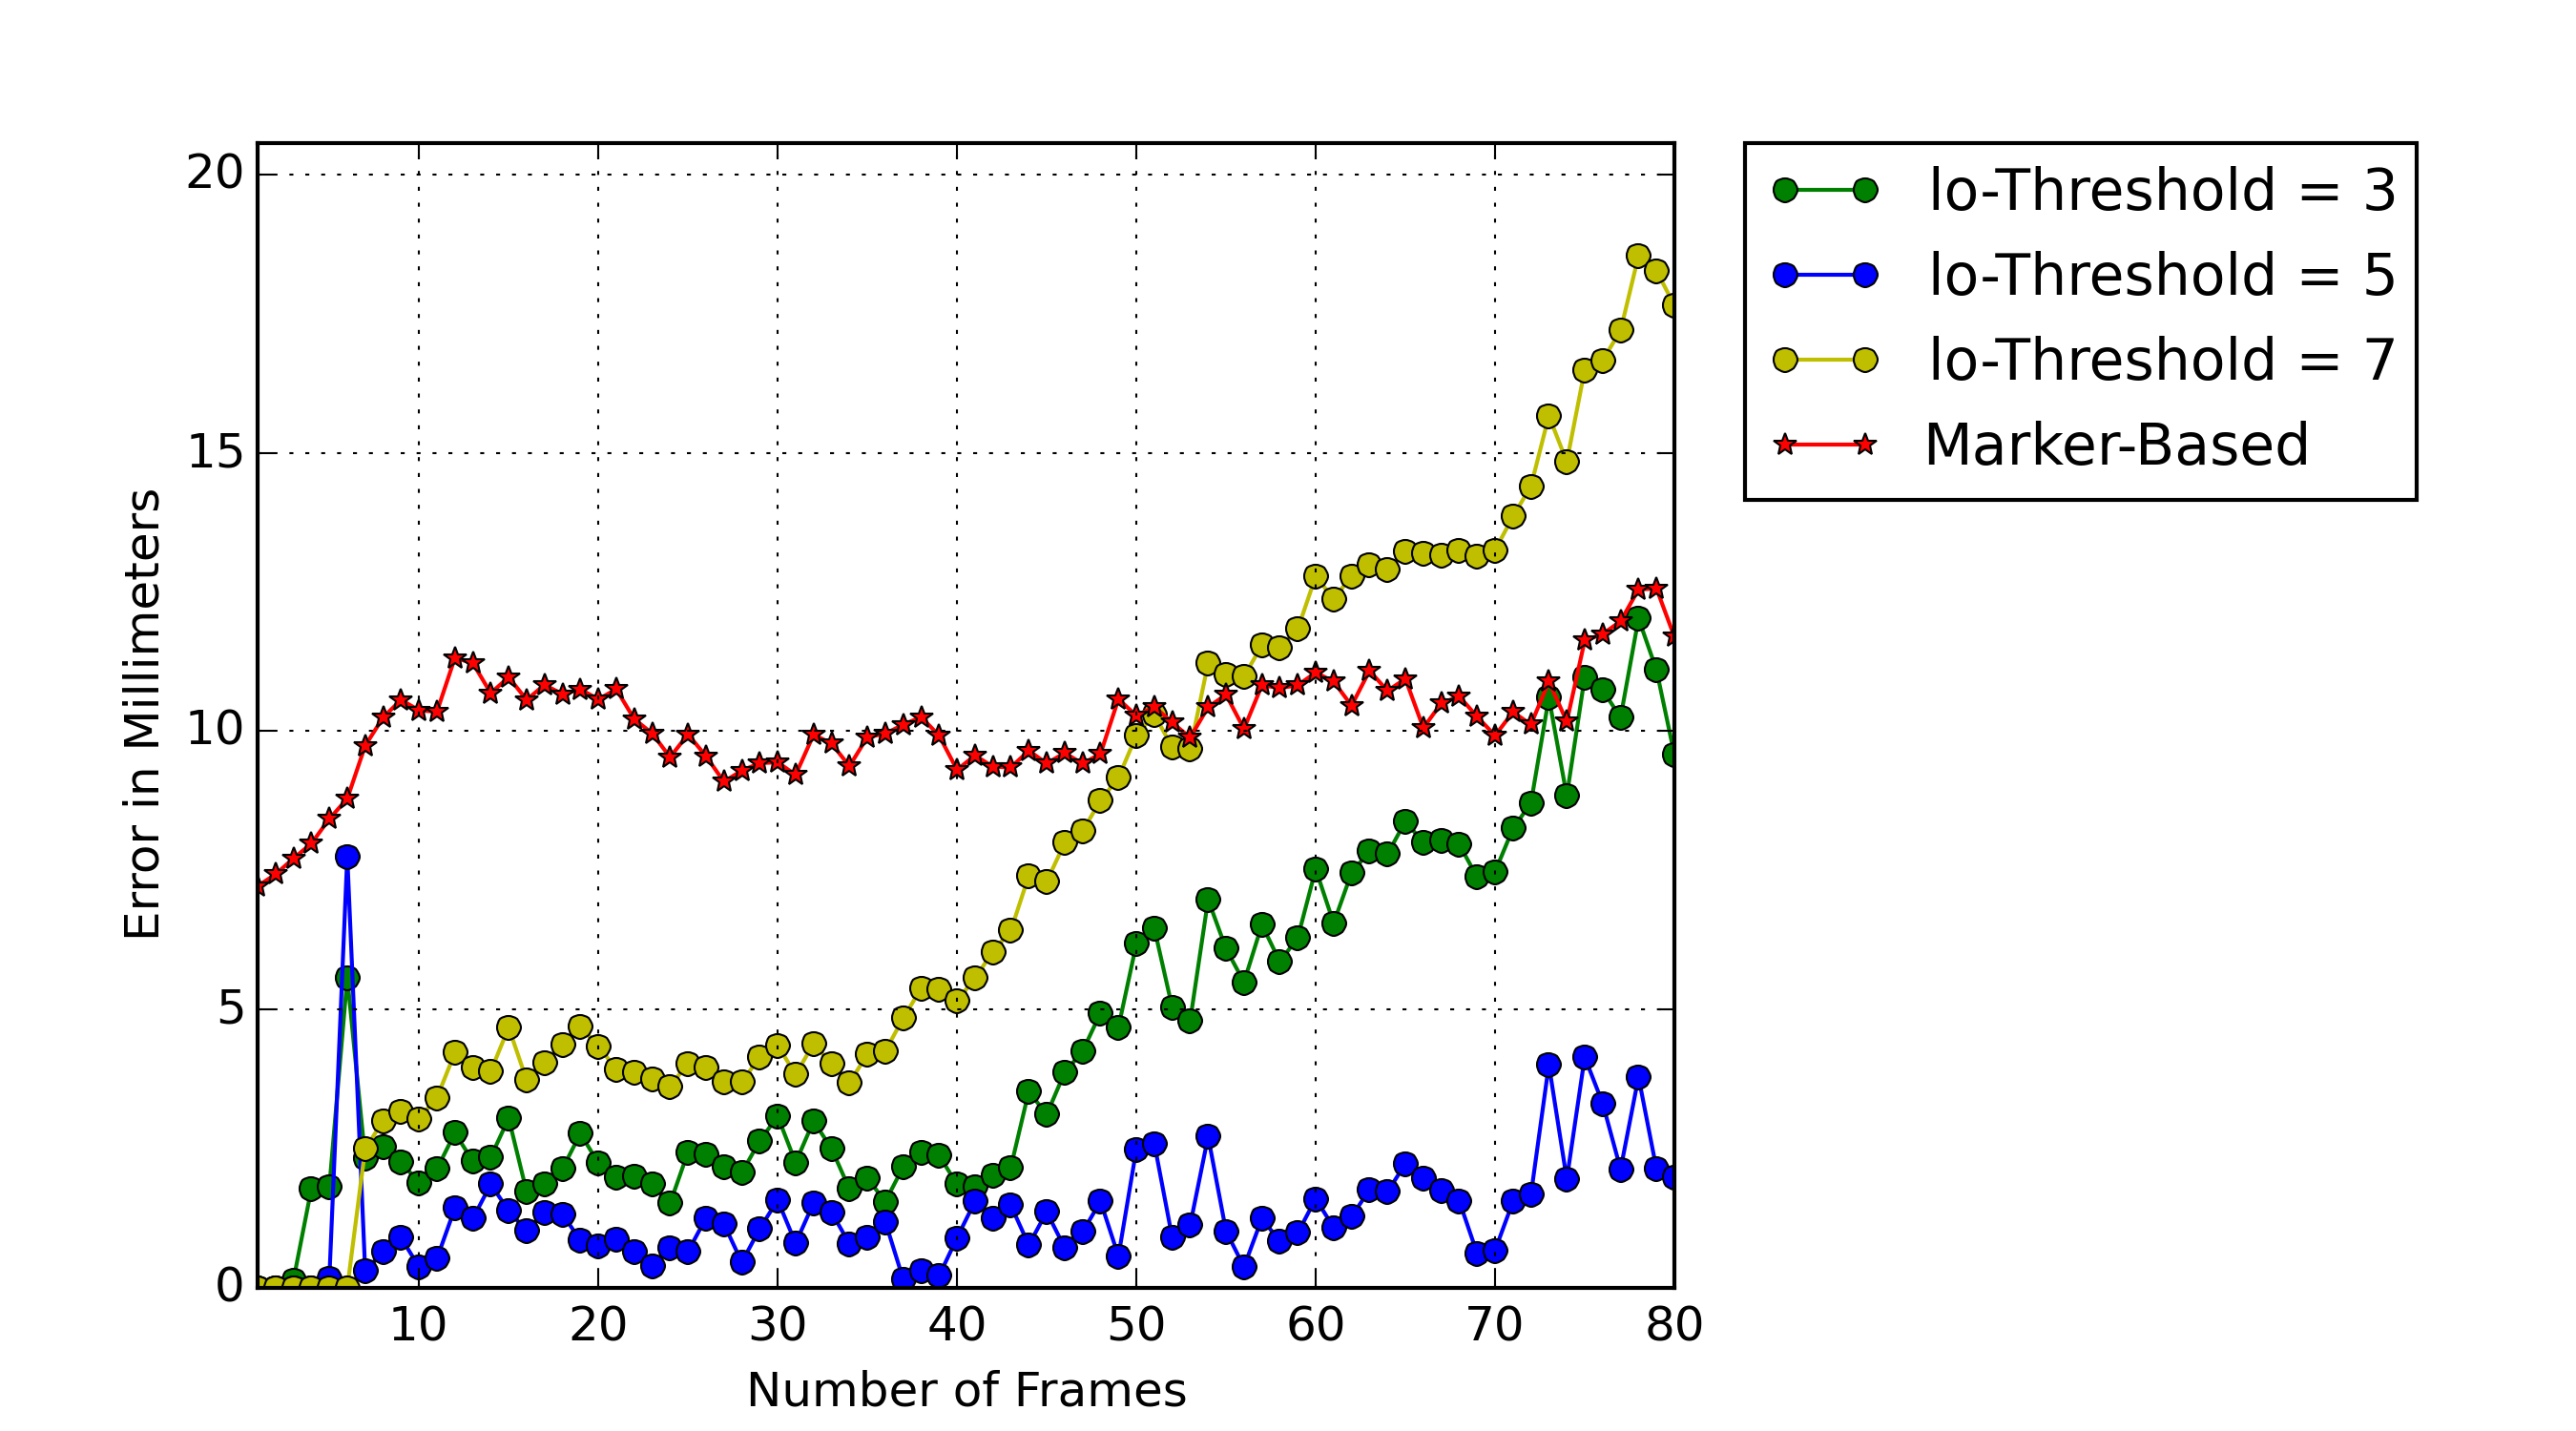
\includegraphics[width=80mm]{figures/local/graph_translation} &   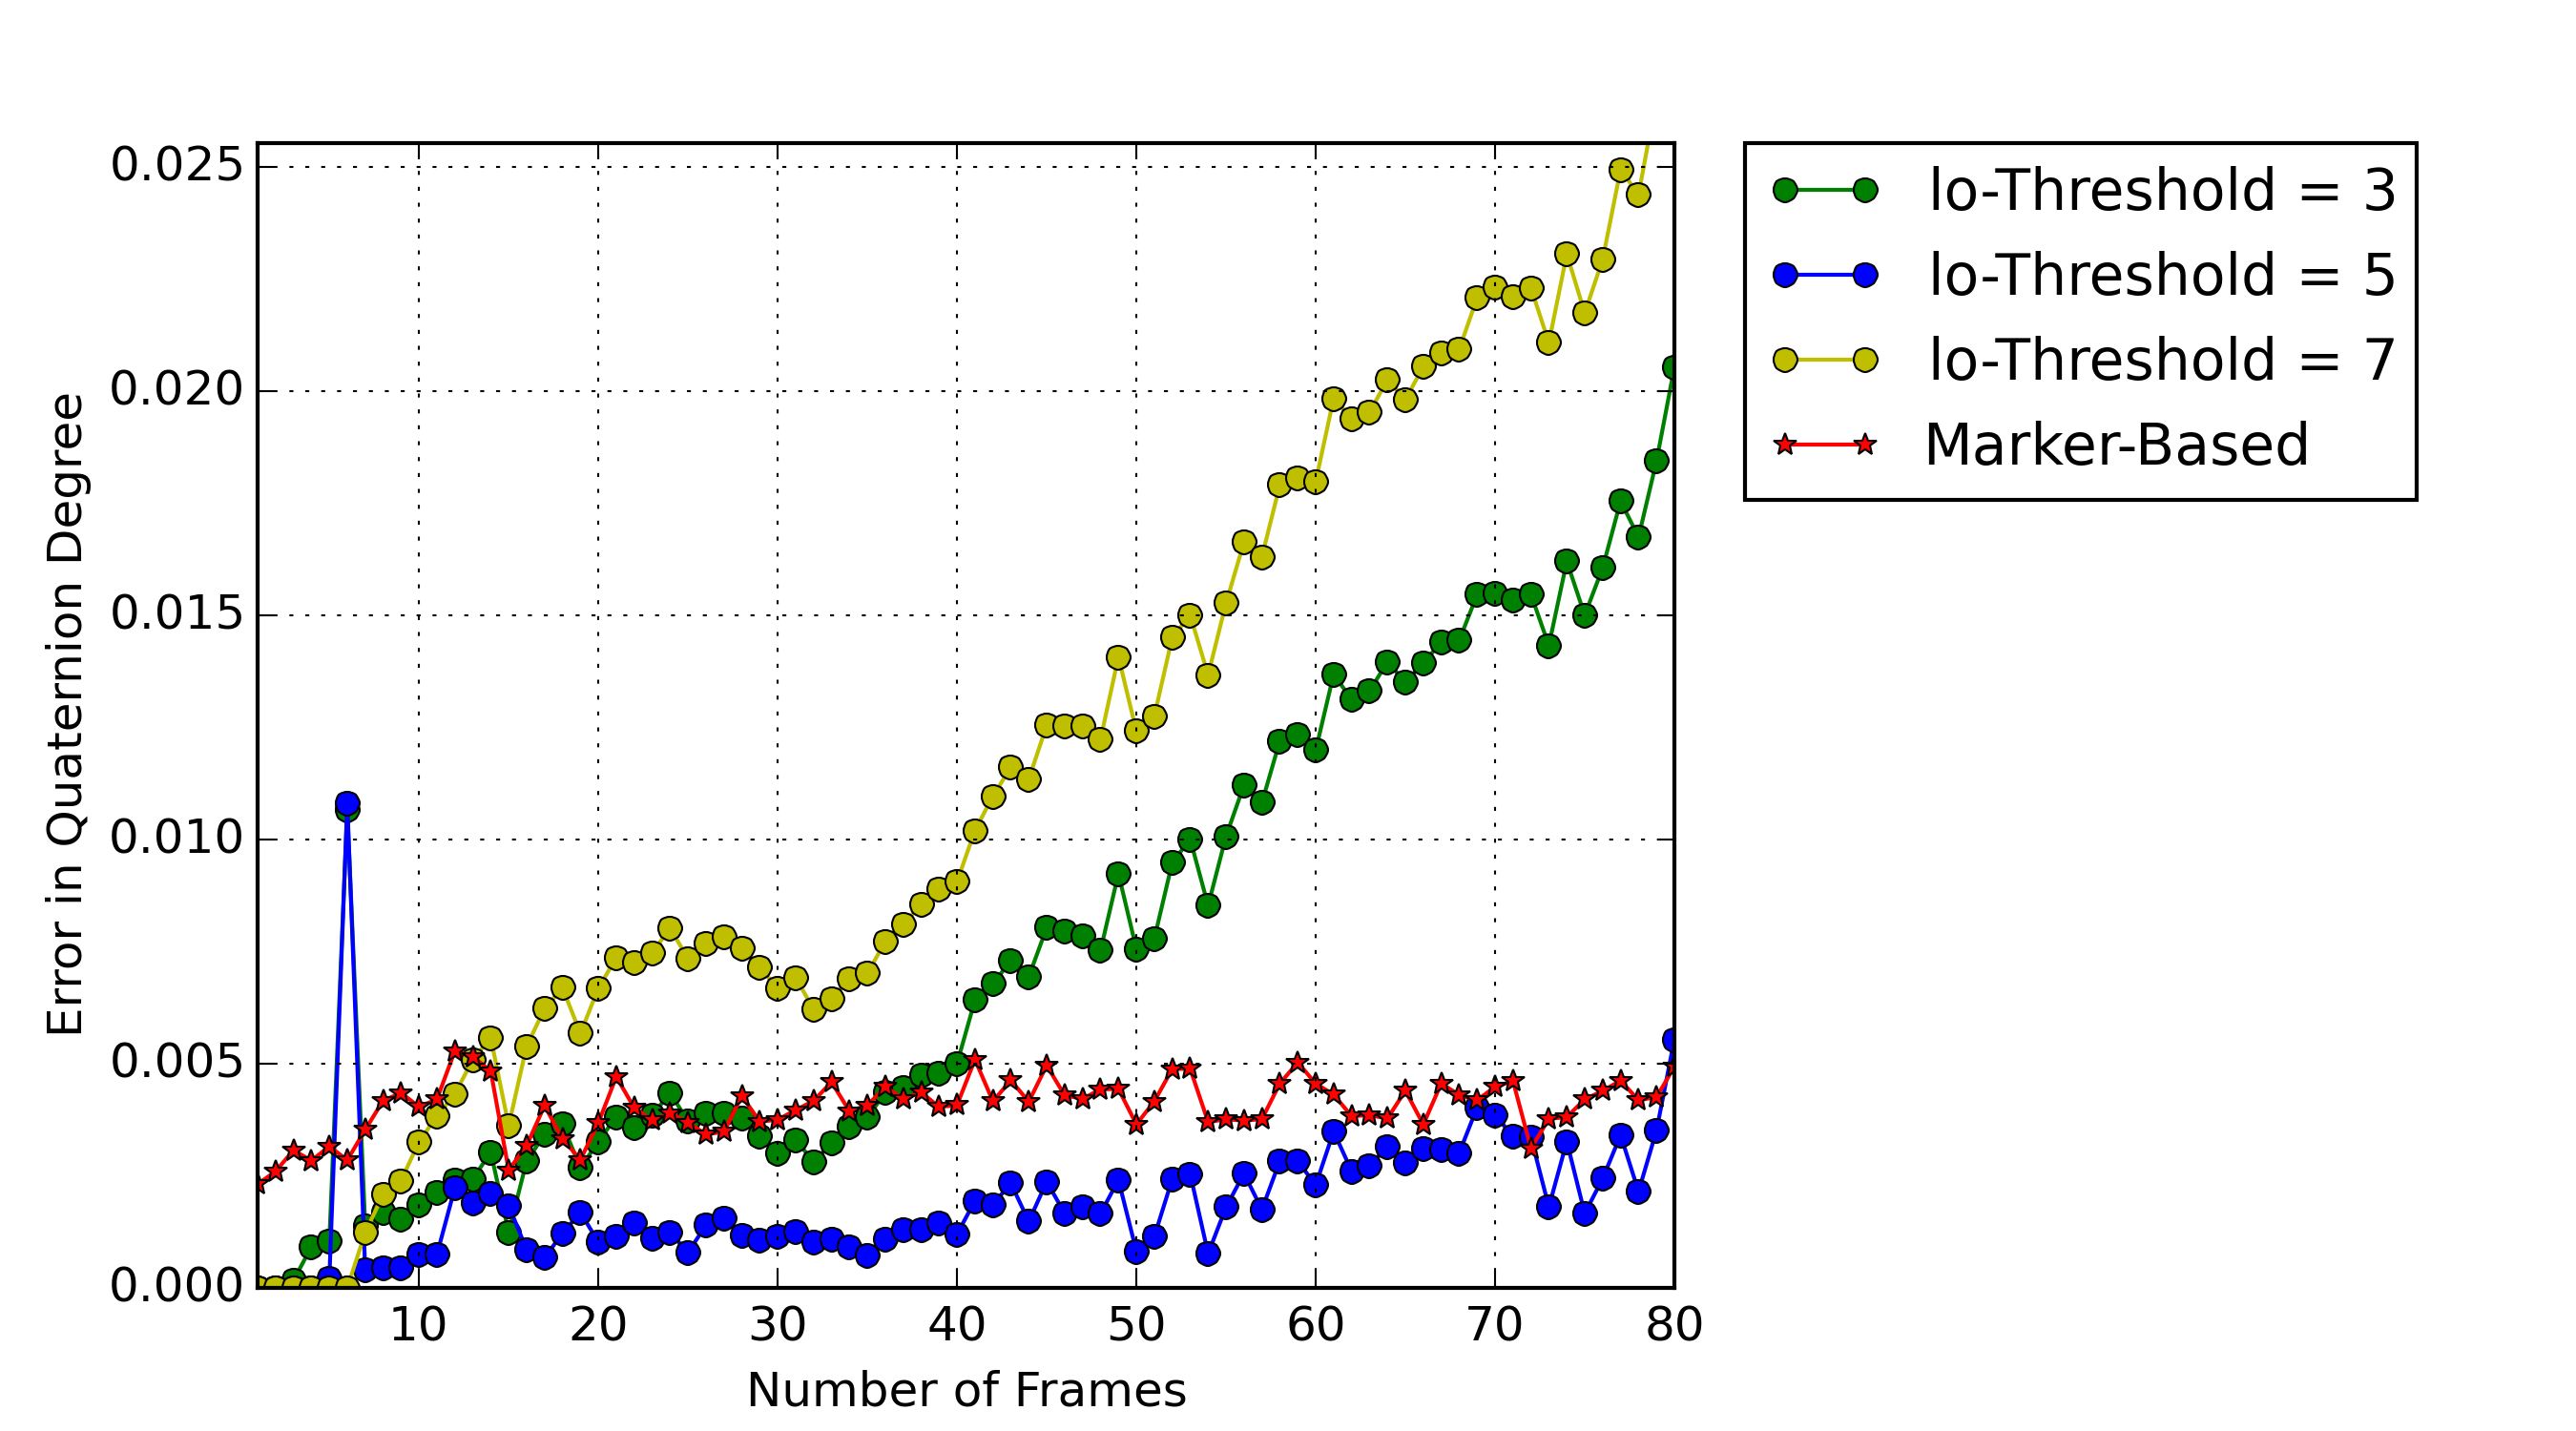
\includegraphics[width=80mm]{figures/local/graph_rotation}  \\
  the translation error & the rotation error \\[6pt]
\end{tabular}
\caption{The translation and rotation error for marker-based Ubitrack method and feature-based with a variety of values for local threshold}\label{fig:test_local_threshold}
\end{figure}

\begin{table}[H]
\centering
  \begin{tabular}{| c || c | c | c | c |}
      \hline
      & \multicolumn{2}{c|}{Translation} & \multicolumn{2}{c|}{Rotation} \\ \hline
       & Mean & Standard Deviation & Mean & Standard Deviation \\ \hline
      Local Threshold = 3 & 4.5165 & 3.0451 & 0.0076 & 0.0054 \\ \hline
      Local Threshold = 5 & \textbf{1.3303} & 1.1184 & \textbf{0.0019} & 0.0015 \\ \hline
      Local Threshold = 7 & 7.7309 & 5.0268 & 0.0117 & 0.0075 \\ \hline
      Marker-Based Ubitrack & 10.1552 & \textbf{0.9700} & 0.0040 & \textbf{0.0006} \\ \hline
  \end{tabular}
  \caption{The statistical analysis of feature-based with different values for local threshold} \label{tab:test_local_threshold}
\end{table}

According to \autoref{tab:test_local_threshold} and \autoref{fig:test_local_threshold}, obviously for both translation and rotation tests, the local threshold with size 5 has the best result where the mean of translation is 1.3303 millimeters and for the rotation is 0.0019 degree of quaternion. To select the second best candidate approach, although the rotation of marker-based approach is 0.0040, but regarding the translation and rotation factors, the local threshold with size 3 is selected as the second best one. It is notable that for both translation and rotation, the marker-based method has the lowest value of standard deviation and consequently it means that the marker-based approach has the highest stability among all methods.

\section{Test Global Threshold} \label{sec:global_threshold}
The next threshold in our approach is about the number of frames that we process for the global bundle adjustment and updating the 3D points in world map vector (\autoref{subsec:update_3d_points}). After each global threshold, the 3D points in world map are completely replaced with the new data points.
\begin{figure}[H]
\centering
\begin{tabular}{cc}
  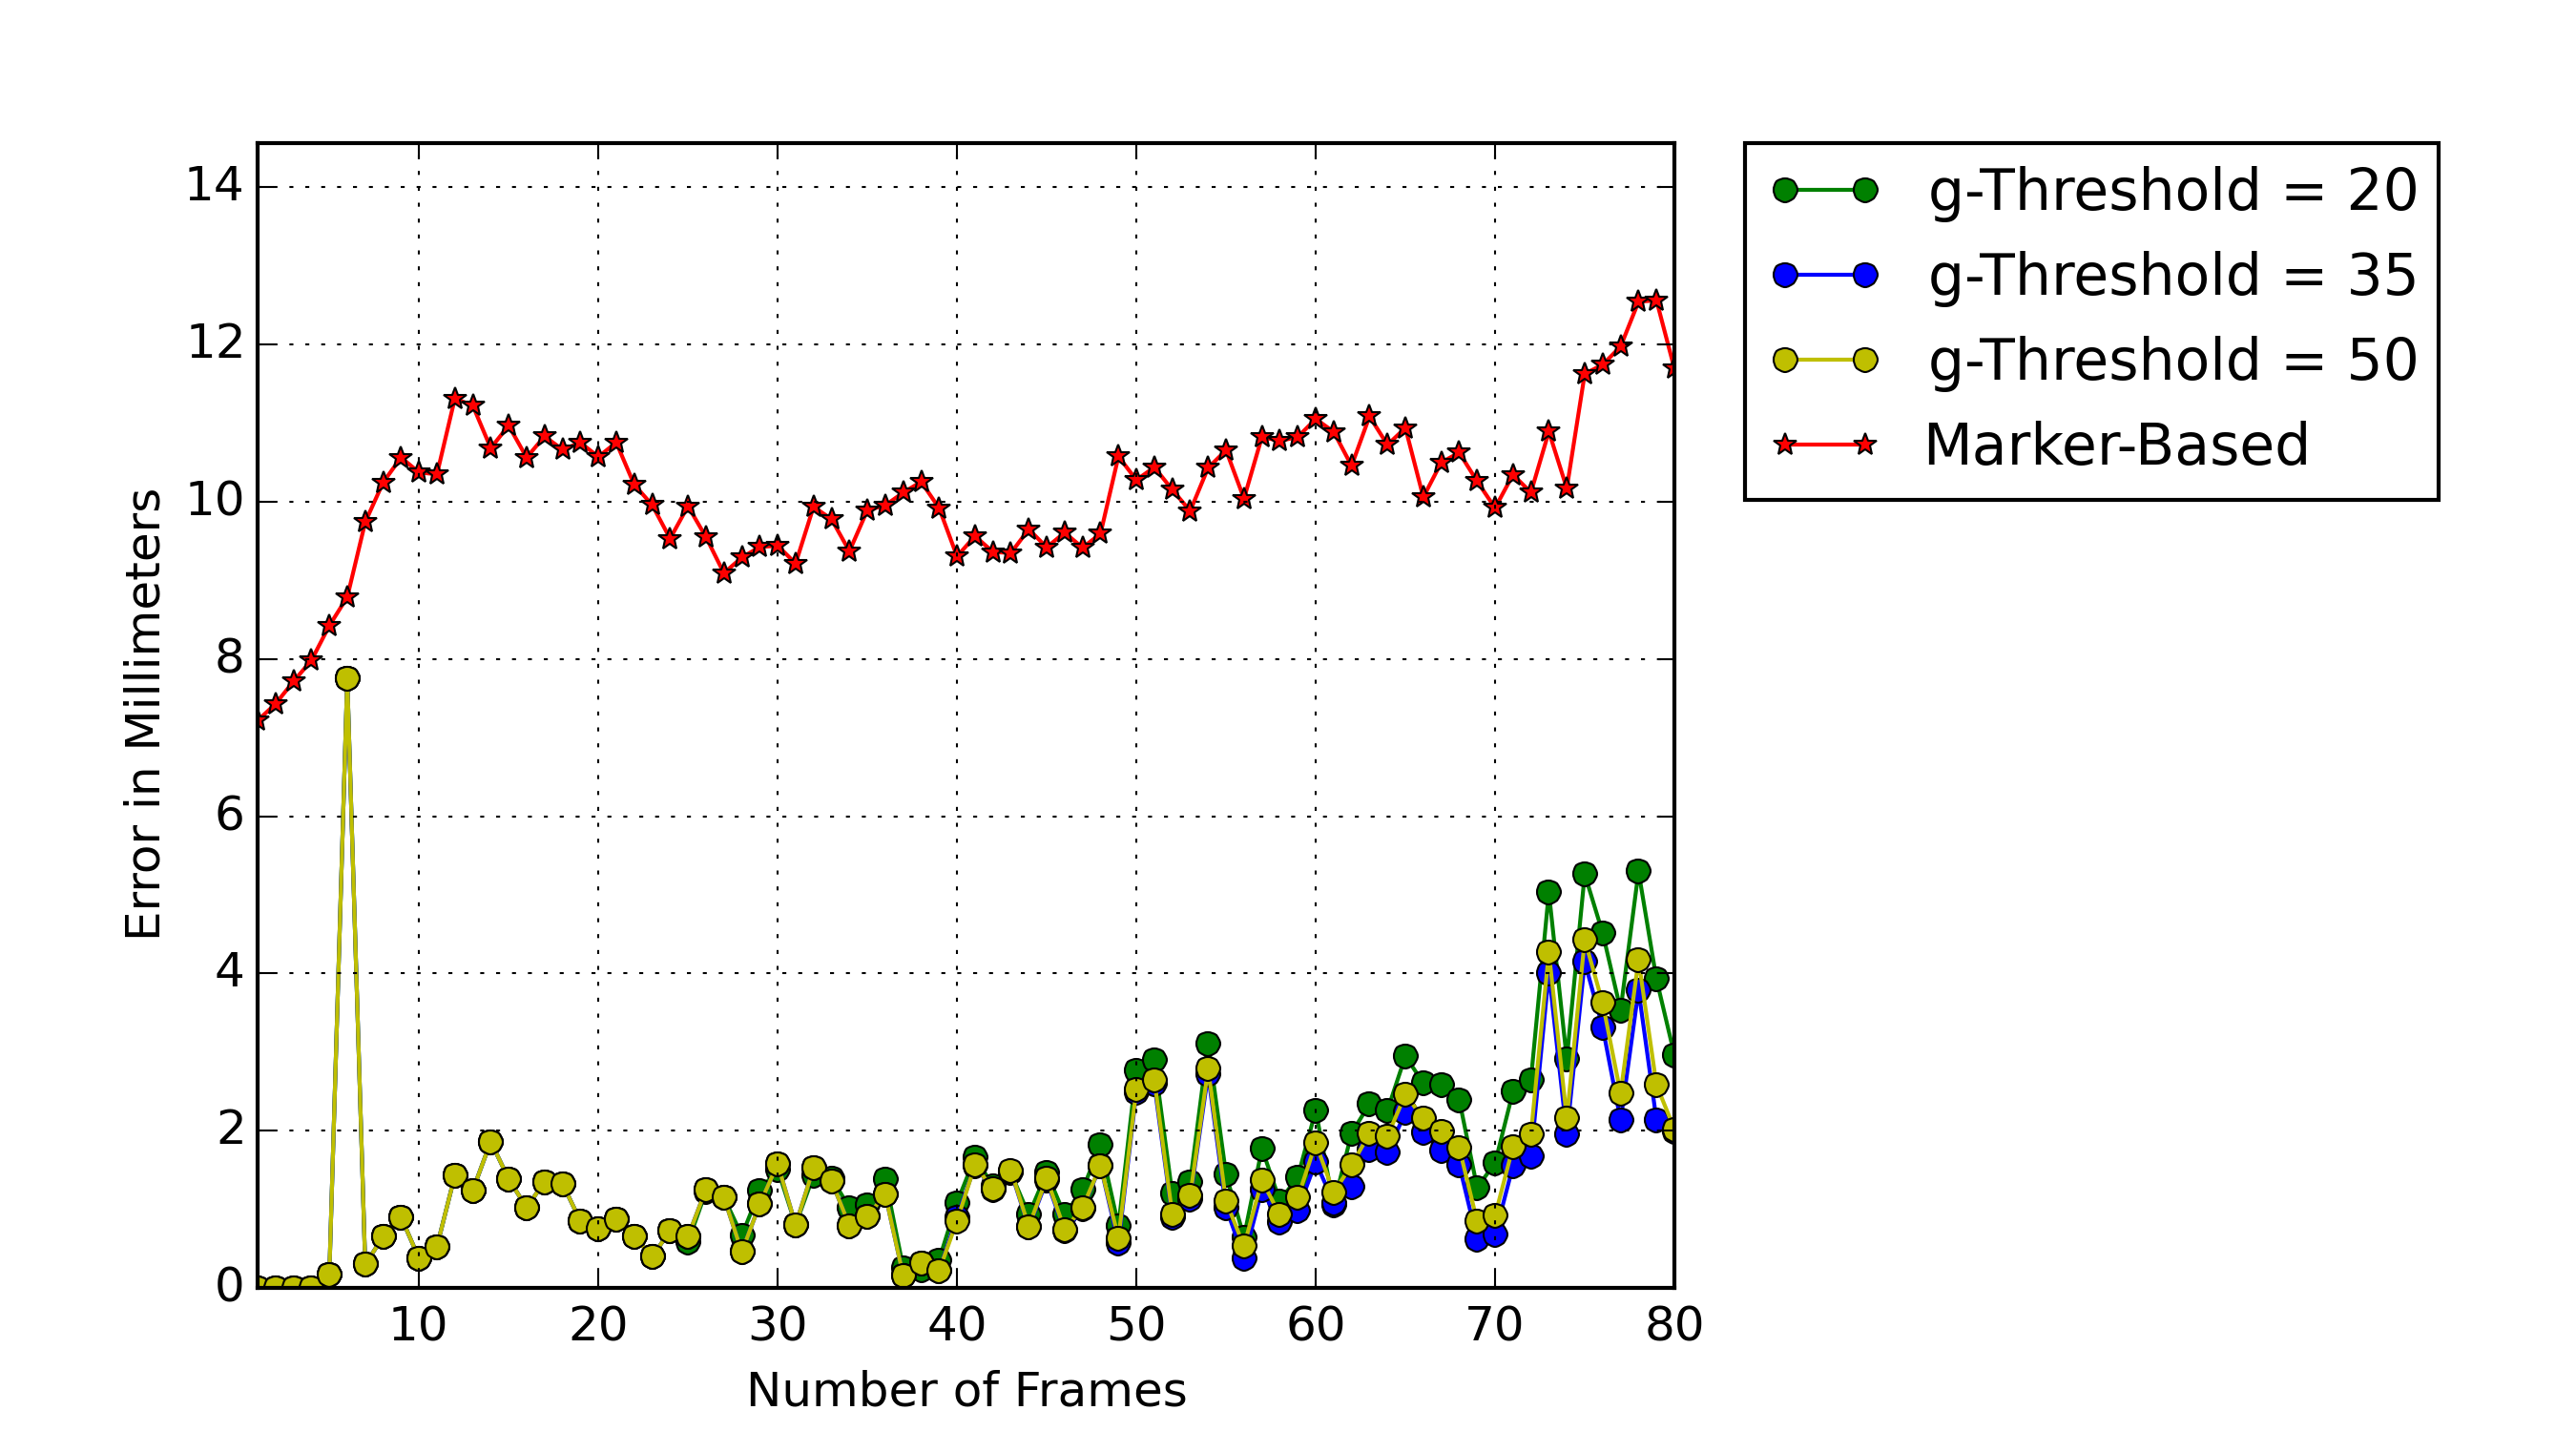
\includegraphics[width=80mm]{figures/global/graph_translation} &   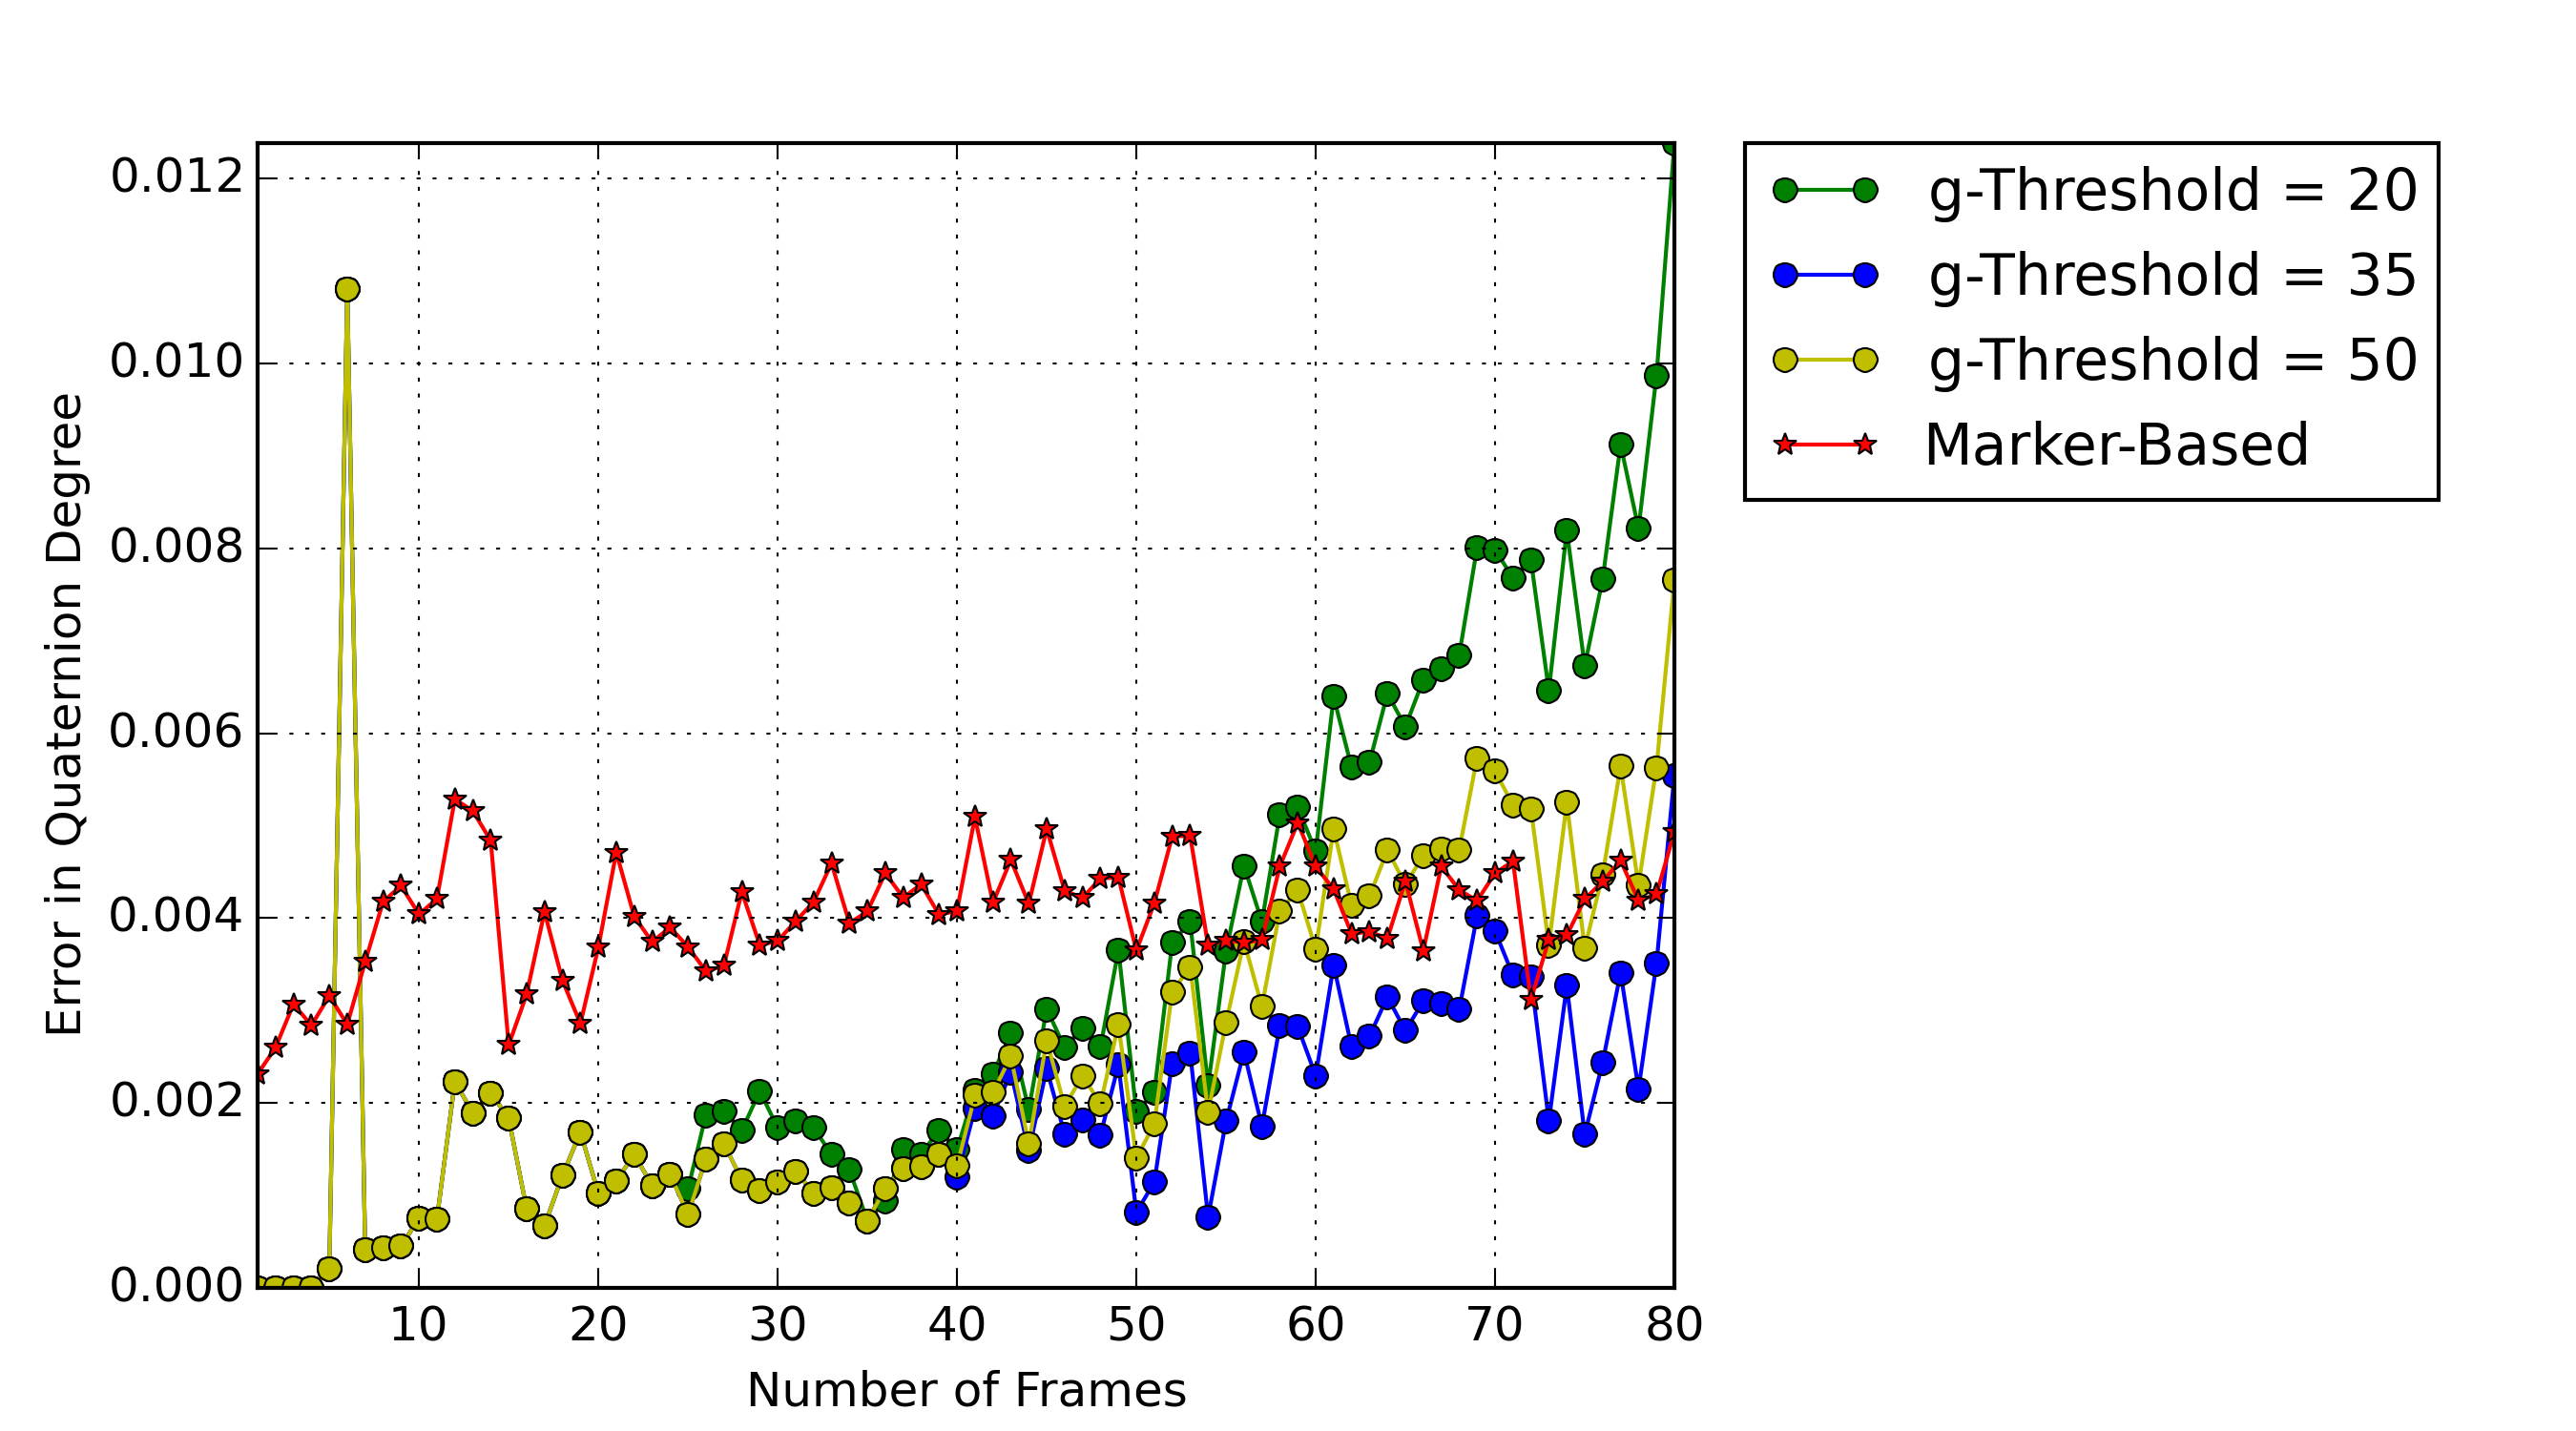
\includegraphics[width=80mm]{figures/global/graph_rotation}  \\
  the translation error & the rotation error \\[6pt]
\end{tabular}
\caption{}\label{fig:test_global_threshold}

\end{figure}
\begin{table}[H]
\centering
  \begin{tabular}{| c || c | c | c | c |}
      \hline
      & \multicolumn{2}{c|}{Translation} & \multicolumn{2}{c|}{Rotation} \\ \hline
       & Mean & Standard Deviation & Mean & Standard Deviation \\ \hline
      Global Threshold = 20 & 1.6392 & 1.3589 & 0.0034 & 0.0029 \\ \hline
      Global Threshold = 35 & \textbf{1.3303} & 1.1184 & \textbf{0.0019} & 0.0015 \\ \hline
      Global Threshold = 50 & 1.4071 & 1.1697 & 0.0025 & 0.0020 \\ \hline
      Marker-based Ubitrack & 10.1552 & \textbf{0.9700} & 0.0040 & \textbf{0.0006} \\ \hline
  \end{tabular}
  \caption{The statistical analysis of feature-based with different values for global threshold} \label{tab:test_global_threshold}
\end{table}
The result of global threshold for all cases 20, 35 and 50 are mostly close together. In fact, the result of all values for tracking are the same whereas the result of global threshold 35 has the best result for rotation. Similar to the local threshold, in this test also the marker-based has the lowest standard deviation among all methods that were tested.

\section{Computing the initial Pose} \label{sec:initial_pose}
In \autoref{subsec:pose_first_bundle}, we introduced two methods for computing the camera poses of first bundle in feature-based approach. One in which the initial poses are taken form the reference system (reference initialization) or the other method in which the initial poses are computed by the planner tracking and homography matrices (Homography initialization).

As can be seen in \autoref{fig:initial_pose} and based on the \autoref{tab:initial_pose}, the reference initialization is significantly better than the other methods. The reason for this is, in the reference initialization method, because the camera poses are accurate enough, consequently the 3D world map is also created precisely. When we use the planner tracking for estimating the pose, for the first five frames the estimated poses are noisy and unstable but after that the translation error decreases smoothly to finally reach to minimum value at \nth{40} frame.

Due to the error of rotation and its negative effect on the local and global bundle adjustment, the errors of rotation and translation have a dramatic increase whereas in the final frame (80), the errors are around 0.027 and 23 millimeters respectively. 

\begin{figure}[H]
\begin{tabular}{cc}
  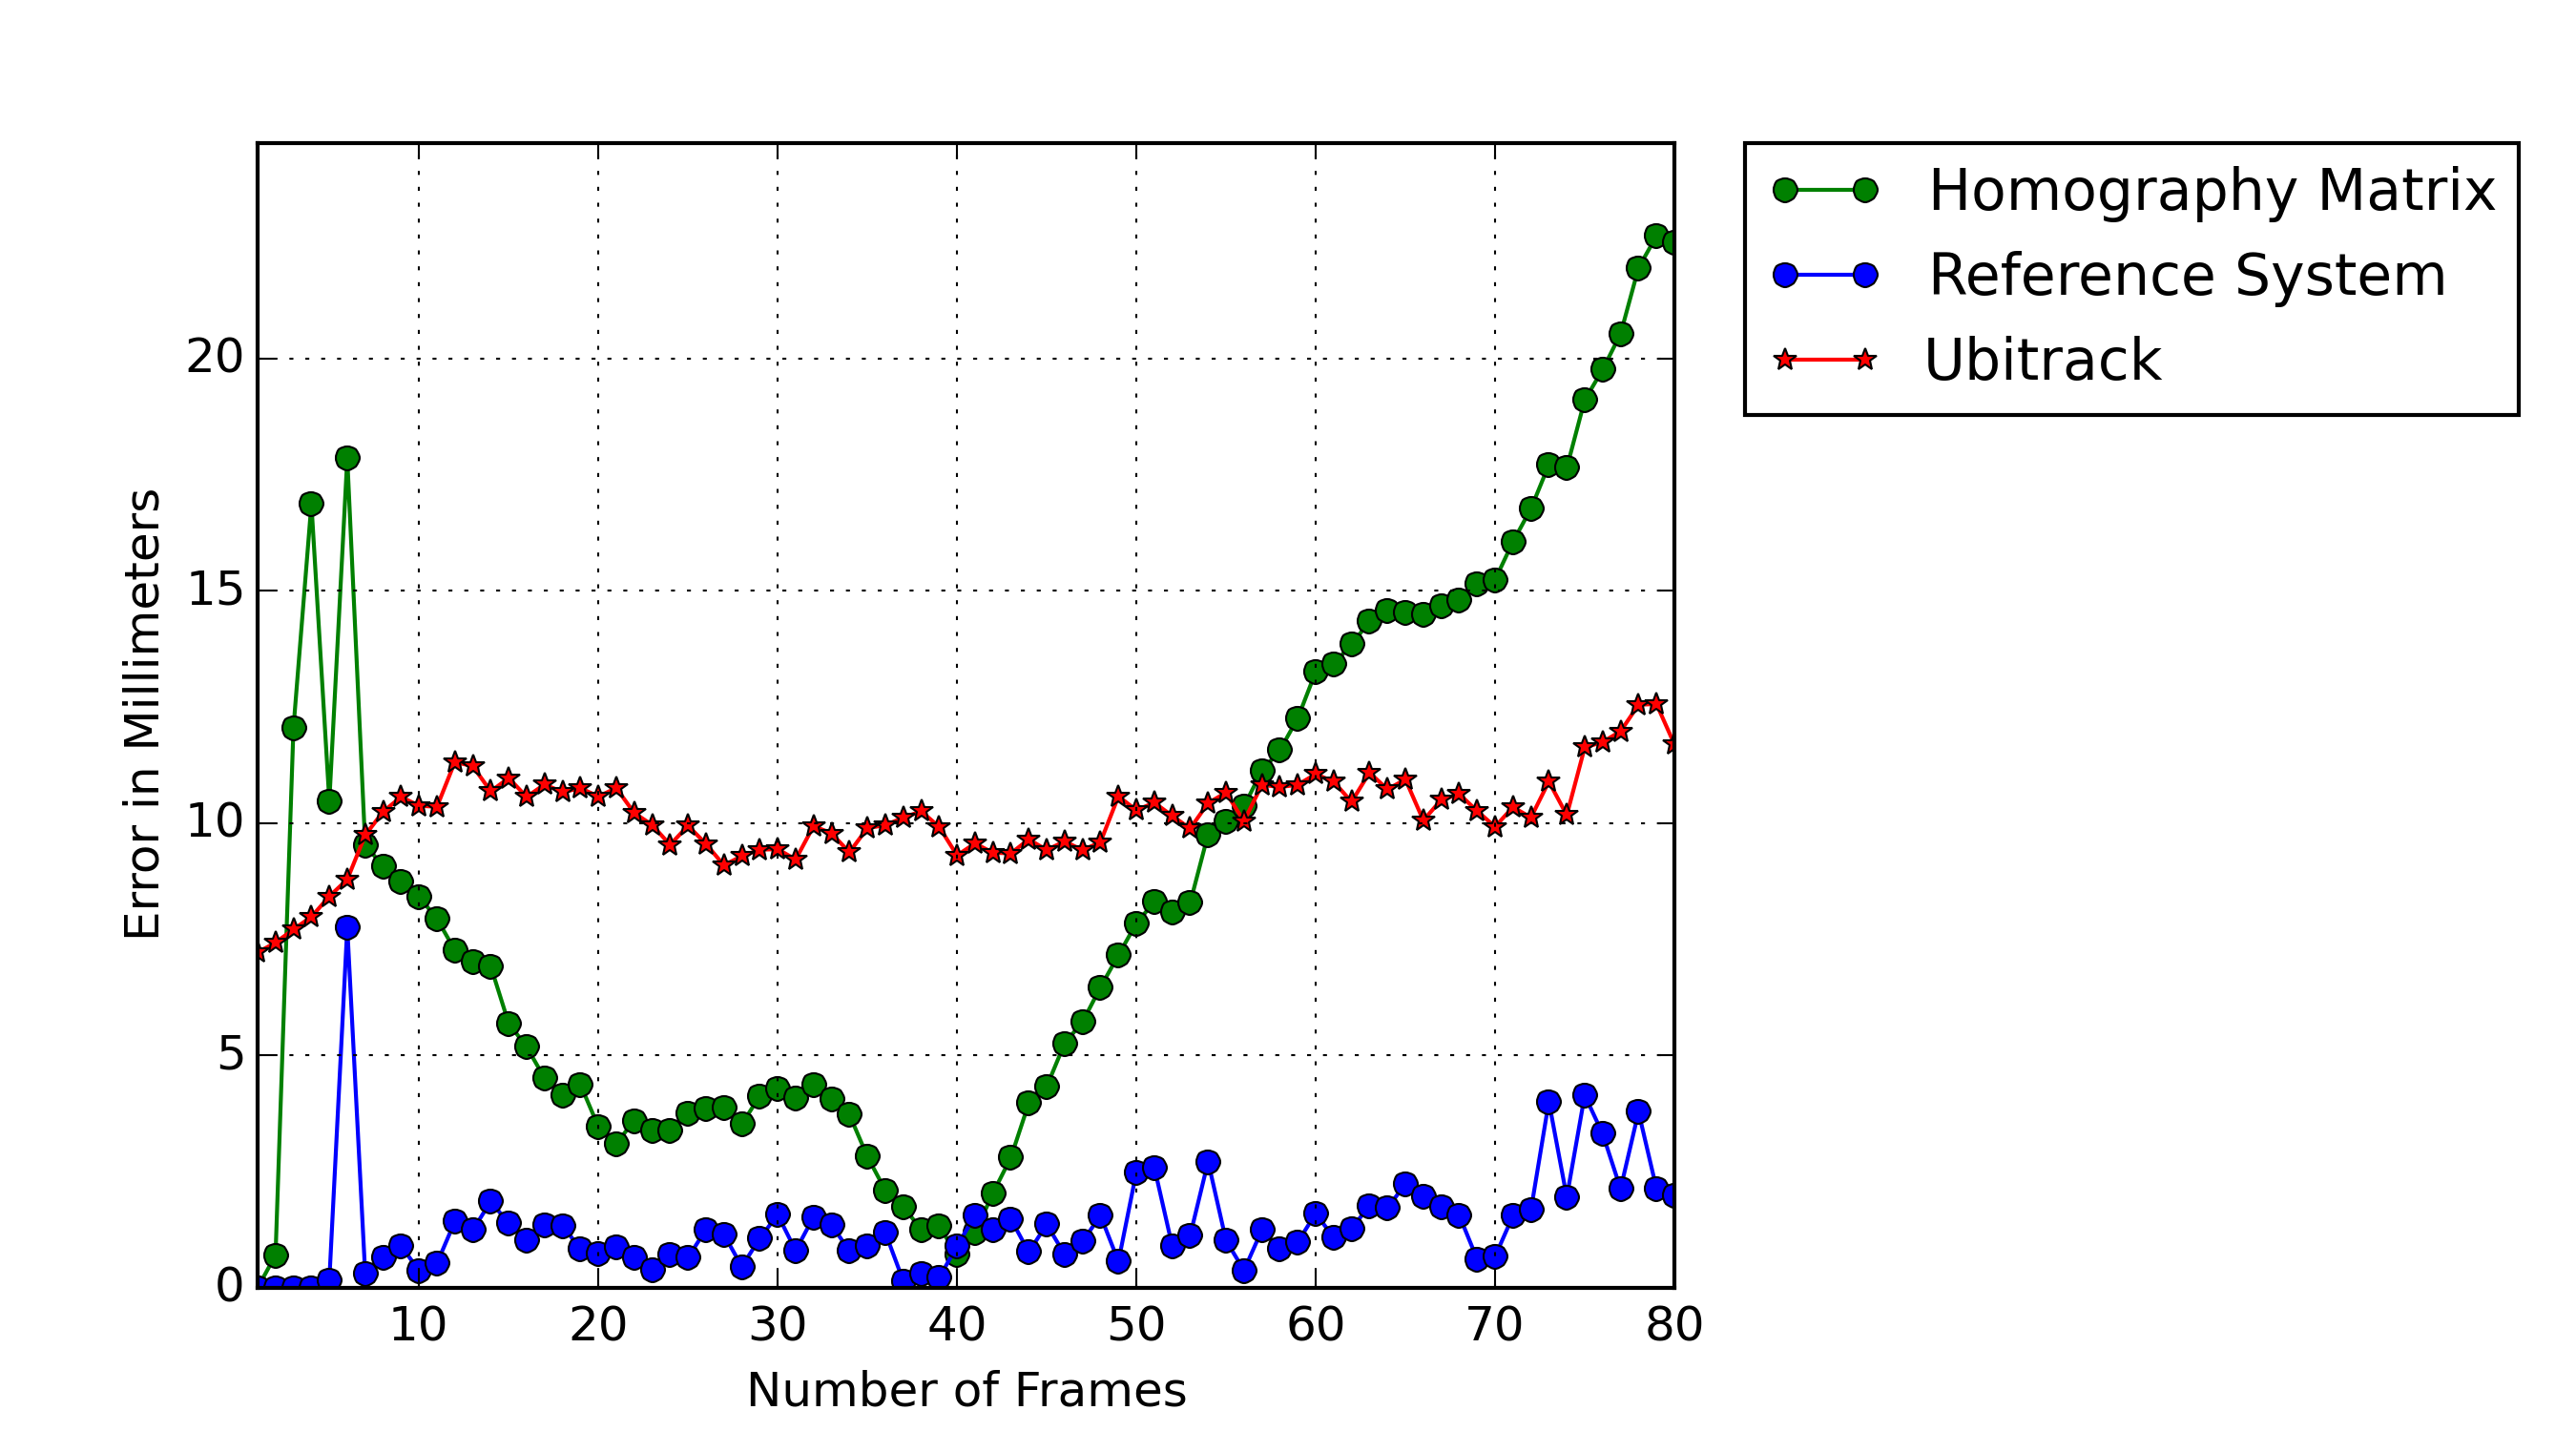
\includegraphics[width=80mm]{figures/homo/graph_translation} &  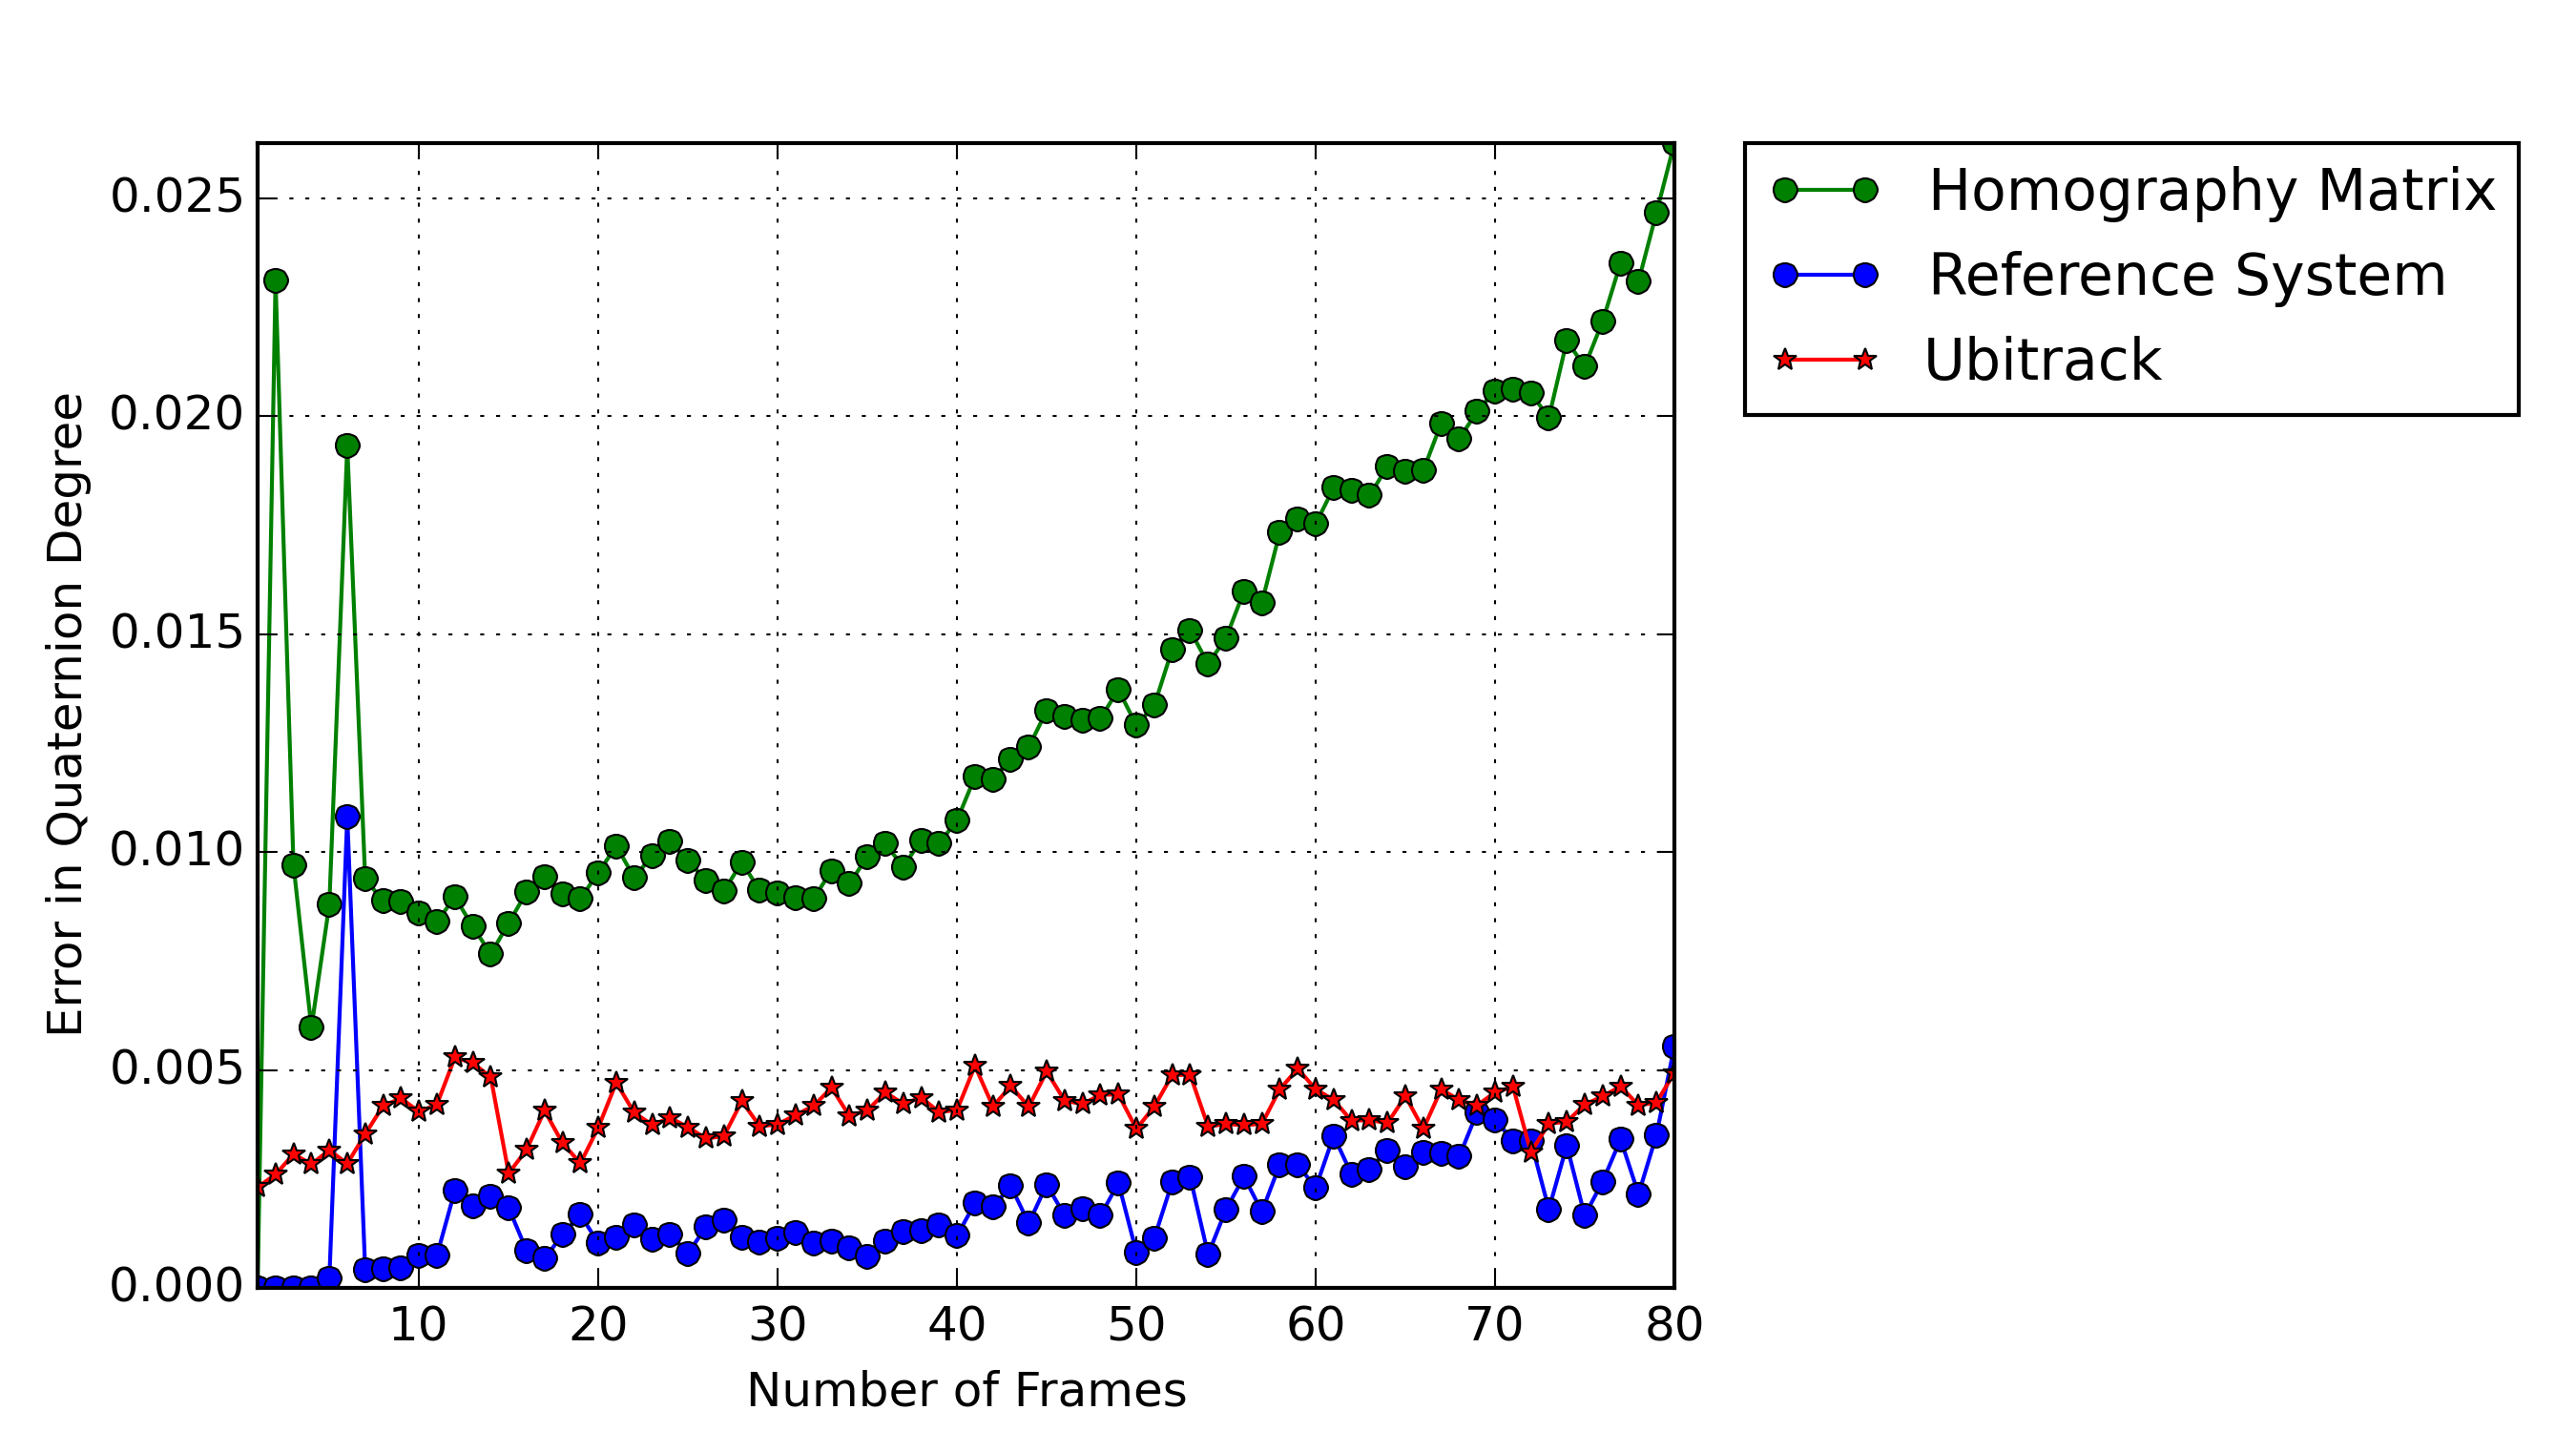
\includegraphics[width=80mm]{figures/homo/graph_rotation} \\
	(a) The translation error & (b) The rotation error \\[6pt]
\end{tabular}
\caption{The comparison of result of methods that use for computing the camera reference pose }\label{fig:initial_pose}
\end{figure}

\begin{table}[H]
\centering
  \begin{tabular}{| c || c | c | c | c |}
      \hline
      & \multicolumn{2}{c|}{Translation} & \multicolumn{2}{c|}{Rotation} \\ \hline
       & Mean & Standard Deviation & Mean & Standard Deviation \\ \hline
      Homography Matrix & 8.7867 & 5.9866 & 0.0135 & 0.0053 \\ \hline
      Reference System & \textbf{1.3303} & 1.1184 & \textbf{0.0019} & 0.0015 \\ \hline
      Marker-based Ubitrack & 10.1552 & \textbf{0.9700} & 0.0040 & \textbf{0.0006} \\ \hline
  \end{tabular}
  \caption{The comparison of error of reference initialization and Homography initialization} \label{tab:initial_pose}
\end{table}

